\documentclass[twoside]{book}

% Packages required by doxygen
\usepackage{fixltx2e}
\usepackage{calc}
\usepackage{doxygen}
\usepackage[export]{adjustbox} % also loads graphicx
\usepackage{graphicx}
\usepackage[utf8]{inputenc}
\usepackage{makeidx}
\usepackage{multicol}
\usepackage{multirow}
\PassOptionsToPackage{warn}{textcomp}
\usepackage{textcomp}
\usepackage[nointegrals]{wasysym}
\usepackage[table]{xcolor}

% Font selection
\usepackage[T1]{fontenc}
\usepackage[scaled=.90]{helvet}
\usepackage{courier}
\usepackage{amssymb}
\usepackage{sectsty}
\renewcommand{\familydefault}{\sfdefault}
\allsectionsfont{%
  \fontseries{bc}\selectfont%
  \color{darkgray}%
}
\renewcommand{\DoxyLabelFont}{%
  \fontseries{bc}\selectfont%
  \color{darkgray}%
}
\newcommand{\+}{\discretionary{\mbox{\scriptsize$\hookleftarrow$}}{}{}}

% Page & text layout
\usepackage{geometry}
\geometry{%
  a4paper,%
  top=2.5cm,%
  bottom=2.5cm,%
  left=2.5cm,%
  right=2.5cm%
}
\tolerance=750
\hfuzz=15pt
\hbadness=750
\setlength{\emergencystretch}{15pt}
\setlength{\parindent}{0cm}
\setlength{\parskip}{3ex plus 2ex minus 2ex}
\makeatletter
\renewcommand{\paragraph}{%
  \@startsection{paragraph}{4}{0ex}{-1.0ex}{1.0ex}{%
    \normalfont\normalsize\bfseries\SS@parafont%
  }%
}
\renewcommand{\subparagraph}{%
  \@startsection{subparagraph}{5}{0ex}{-1.0ex}{1.0ex}{%
    \normalfont\normalsize\bfseries\SS@subparafont%
  }%
}
\makeatother

% Headers & footers
\usepackage{fancyhdr}
\pagestyle{fancyplain}
\fancyhead[LE]{\fancyplain{}{\bfseries\thepage}}
\fancyhead[CE]{\fancyplain{}{}}
\fancyhead[RE]{\fancyplain{}{\bfseries\leftmark}}
\fancyhead[LO]{\fancyplain{}{\bfseries\rightmark}}
\fancyhead[CO]{\fancyplain{}{}}
\fancyhead[RO]{\fancyplain{}{\bfseries\thepage}}
\fancyfoot[LE]{\fancyplain{}{}}
\fancyfoot[CE]{\fancyplain{}{}}
\fancyfoot[RE]{\fancyplain{}{\bfseries\scriptsize Generated by Doxygen }}
\fancyfoot[LO]{\fancyplain{}{\bfseries\scriptsize Generated by Doxygen }}
\fancyfoot[CO]{\fancyplain{}{}}
\fancyfoot[RO]{\fancyplain{}{}}
\renewcommand{\footrulewidth}{0.4pt}
\renewcommand{\chaptermark}[1]{%
  \markboth{#1}{}%
}
\renewcommand{\sectionmark}[1]{%
  \markright{\thesection\ #1}%
}

% Indices & bibliography
\usepackage{natbib}
\usepackage[titles]{tocloft}
\setcounter{tocdepth}{3}
\setcounter{secnumdepth}{5}
\makeindex

% Hyperlinks (required, but should be loaded last)
\usepackage{ifpdf}
\ifpdf
  \usepackage[pdftex,pagebackref=true]{hyperref}
\else
  \usepackage[ps2pdf,pagebackref=true]{hyperref}
\fi
\hypersetup{%
  colorlinks=true,%
  linkcolor=blue,%
  citecolor=blue,%
  unicode%
}

% Custom commands
\newcommand{\clearemptydoublepage}{%
  \newpage{\pagestyle{empty}\cleardoublepage}%
}

\usepackage{caption}
\captionsetup{labelsep=space,justification=centering,font={bf},singlelinecheck=off,skip=4pt,position=top}

%===== C O N T E N T S =====

\begin{document}

% Titlepage & ToC
\hypersetup{pageanchor=false,
             bookmarksnumbered=true,
             pdfencoding=unicode
            }
\pagenumbering{roman}
\begin{titlepage}
\vspace*{7cm}
\begin{center}%
{\Large E\+N\+P\+M808\+X-\/\+Midterm-\/\+Informed\+R\+R\+T\+Star }\\
\vspace*{1cm}
{\large Generated by Doxygen 1.8.11}\\
\end{center}
\end{titlepage}
\clearemptydoublepage
\tableofcontents
\clearemptydoublepage
\pagenumbering{arabic}
\hypersetup{pageanchor=true}

%--- Begin generated contents ---
\chapter{Hierarchical Index}
\section{Class Hierarchy}
This inheritance list is sorted roughly, but not completely, alphabetically\+:\begin{DoxyCompactList}
\item \contentsline{section}{matplotlibcpp\+:\+:detail\+:\+:\+\_\+interpreter}{\pageref{structmatplotlibcpp_1_1detail_1_1__interpreter}}{}
\item \contentsline{section}{Map}{\pageref{classMap}}{}
\item \contentsline{section}{R\+RT}{\pageref{classRRT}}{}
\begin{DoxyCompactList}
\item \contentsline{section}{R\+R\+T\+Star}{\pageref{classRRTStar}}{}
\begin{DoxyCompactList}
\item \contentsline{section}{Informed\+R\+R\+T\+Star}{\pageref{classInformedRRTStar}}{}
\end{DoxyCompactList}
\end{DoxyCompactList}
\item \contentsline{section}{R\+R\+T\+Node}{\pageref{classRRTNode}}{}
\item \contentsline{section}{matplotlibcpp\+:\+:select\+\_\+npy\+\_\+type$<$ T $>$}{\pageref{structmatplotlibcpp_1_1select__npy__type}}{}
\item \contentsline{section}{matplotlibcpp\+:\+:select\+\_\+npy\+\_\+type$<$ bool $>$}{\pageref{structmatplotlibcpp_1_1select__npy__type_3_01bool_01_4}}{}
\item \contentsline{section}{matplotlibcpp\+:\+:select\+\_\+npy\+\_\+type$<$ double $>$}{\pageref{structmatplotlibcpp_1_1select__npy__type_3_01double_01_4}}{}
\item \contentsline{section}{matplotlibcpp\+:\+:select\+\_\+npy\+\_\+type$<$ float $>$}{\pageref{structmatplotlibcpp_1_1select__npy__type_3_01float_01_4}}{}
\item \contentsline{section}{matplotlibcpp\+:\+:select\+\_\+npy\+\_\+type$<$ int16\+\_\+t $>$}{\pageref{structmatplotlibcpp_1_1select__npy__type_3_01int16__t_01_4}}{}
\item \contentsline{section}{matplotlibcpp\+:\+:select\+\_\+npy\+\_\+type$<$ int32\+\_\+t $>$}{\pageref{structmatplotlibcpp_1_1select__npy__type_3_01int32__t_01_4}}{}
\item \contentsline{section}{matplotlibcpp\+:\+:select\+\_\+npy\+\_\+type$<$ int64\+\_\+t $>$}{\pageref{structmatplotlibcpp_1_1select__npy__type_3_01int64__t_01_4}}{}
\item \contentsline{section}{matplotlibcpp\+:\+:select\+\_\+npy\+\_\+type$<$ int8\+\_\+t $>$}{\pageref{structmatplotlibcpp_1_1select__npy__type_3_01int8__t_01_4}}{}
\item \contentsline{section}{matplotlibcpp\+:\+:select\+\_\+npy\+\_\+type$<$ uint16\+\_\+t $>$}{\pageref{structmatplotlibcpp_1_1select__npy__type_3_01uint16__t_01_4}}{}
\item \contentsline{section}{matplotlibcpp\+:\+:select\+\_\+npy\+\_\+type$<$ uint32\+\_\+t $>$}{\pageref{structmatplotlibcpp_1_1select__npy__type_3_01uint32__t_01_4}}{}
\item \contentsline{section}{matplotlibcpp\+:\+:select\+\_\+npy\+\_\+type$<$ uint64\+\_\+t $>$}{\pageref{structmatplotlibcpp_1_1select__npy__type_3_01uint64__t_01_4}}{}
\item \contentsline{section}{matplotlibcpp\+:\+:select\+\_\+npy\+\_\+type$<$ uint8\+\_\+t $>$}{\pageref{structmatplotlibcpp_1_1select__npy__type_3_01uint8__t_01_4}}{}
\end{DoxyCompactList}

\chapter{Class Index}
\section{Class List}
Here are the classes, structs, unions and interfaces with brief descriptions\+:\begin{DoxyCompactList}
\item\contentsline{section}{\hyperlink{structmatplotlibcpp_1_1detail_1_1__interpreter}{matplotlibcpp\+::detail\+::\+\_\+interpreter} }{\pageref{structmatplotlibcpp_1_1detail_1_1__interpreter}}{}
\item\contentsline{section}{\hyperlink{classInformedRRTStar}{Informed\+R\+R\+T\+Star} \\*Class Informed \hyperlink{classRRT}{R\+RT} Star, derived from class \hyperlink{classRRT}{R\+RT} Star The following class \hyperlink{classRRT}{R\+RT} Star converges faster to find the optimized path found by \hyperlink{classRRT}{R\+RT} Star algorithm using a heuristic model }{\pageref{classInformedRRTStar}}{}
\item\contentsline{section}{\hyperlink{classMap}{Map} \\*Class \hyperlink{classMap}{Map} The following class \hyperlink{classMap}{Map} aids in storing the layout of the environment }{\pageref{classMap}}{}
\item\contentsline{section}{\hyperlink{classRRT}{R\+RT} \\*Class \hyperlink{classRRT}{R\+RT} The following class \hyperlink{classRRT}{R\+RT} implements the Rapidly-\/exploring random tree to find a path from start to goal in an environment }{\pageref{classRRT}}{}
\item\contentsline{section}{\hyperlink{classRRTNode}{R\+R\+T\+Node} \\*Class \hyperlink{classRRTNode}{R\+R\+T\+Node} The following class \hyperlink{classRRTNode}{R\+R\+T\+Node} is used to hold information of a node in the tree formed by \hyperlink{classRRT}{R\+RT} algorithm }{\pageref{classRRTNode}}{}
\item\contentsline{section}{\hyperlink{classRRTStar}{R\+R\+T\+Star} \\*Class \hyperlink{classRRT}{R\+RT}, derived from class \hyperlink{classRRT}{R\+RT} The following class \hyperlink{classRRT}{R\+RT} Star optimizes the path found by \hyperlink{classRRT}{R\+RT} algorithm using cost to come to rewire the path and the tree nodes as well }{\pageref{classRRTStar}}{}
\item\contentsline{section}{\hyperlink{structmatplotlibcpp_1_1select__npy__type}{matplotlibcpp\+::select\+\_\+npy\+\_\+type$<$ T $>$} }{\pageref{structmatplotlibcpp_1_1select__npy__type}}{}
\item\contentsline{section}{\hyperlink{structmatplotlibcpp_1_1select__npy__type_3_01bool_01_4}{matplotlibcpp\+::select\+\_\+npy\+\_\+type$<$ bool $>$} }{\pageref{structmatplotlibcpp_1_1select__npy__type_3_01bool_01_4}}{}
\item\contentsline{section}{\hyperlink{structmatplotlibcpp_1_1select__npy__type_3_01double_01_4}{matplotlibcpp\+::select\+\_\+npy\+\_\+type$<$ double $>$} }{\pageref{structmatplotlibcpp_1_1select__npy__type_3_01double_01_4}}{}
\item\contentsline{section}{\hyperlink{structmatplotlibcpp_1_1select__npy__type_3_01float_01_4}{matplotlibcpp\+::select\+\_\+npy\+\_\+type$<$ float $>$} }{\pageref{structmatplotlibcpp_1_1select__npy__type_3_01float_01_4}}{}
\item\contentsline{section}{\hyperlink{structmatplotlibcpp_1_1select__npy__type_3_01int16__t_01_4}{matplotlibcpp\+::select\+\_\+npy\+\_\+type$<$ int16\+\_\+t $>$} }{\pageref{structmatplotlibcpp_1_1select__npy__type_3_01int16__t_01_4}}{}
\item\contentsline{section}{\hyperlink{structmatplotlibcpp_1_1select__npy__type_3_01int32__t_01_4}{matplotlibcpp\+::select\+\_\+npy\+\_\+type$<$ int32\+\_\+t $>$} }{\pageref{structmatplotlibcpp_1_1select__npy__type_3_01int32__t_01_4}}{}
\item\contentsline{section}{\hyperlink{structmatplotlibcpp_1_1select__npy__type_3_01int64__t_01_4}{matplotlibcpp\+::select\+\_\+npy\+\_\+type$<$ int64\+\_\+t $>$} }{\pageref{structmatplotlibcpp_1_1select__npy__type_3_01int64__t_01_4}}{}
\item\contentsline{section}{\hyperlink{structmatplotlibcpp_1_1select__npy__type_3_01int8__t_01_4}{matplotlibcpp\+::select\+\_\+npy\+\_\+type$<$ int8\+\_\+t $>$} }{\pageref{structmatplotlibcpp_1_1select__npy__type_3_01int8__t_01_4}}{}
\item\contentsline{section}{\hyperlink{structmatplotlibcpp_1_1select__npy__type_3_01uint16__t_01_4}{matplotlibcpp\+::select\+\_\+npy\+\_\+type$<$ uint16\+\_\+t $>$} }{\pageref{structmatplotlibcpp_1_1select__npy__type_3_01uint16__t_01_4}}{}
\item\contentsline{section}{\hyperlink{structmatplotlibcpp_1_1select__npy__type_3_01uint32__t_01_4}{matplotlibcpp\+::select\+\_\+npy\+\_\+type$<$ uint32\+\_\+t $>$} }{\pageref{structmatplotlibcpp_1_1select__npy__type_3_01uint32__t_01_4}}{}
\item\contentsline{section}{\hyperlink{structmatplotlibcpp_1_1select__npy__type_3_01uint64__t_01_4}{matplotlibcpp\+::select\+\_\+npy\+\_\+type$<$ uint64\+\_\+t $>$} }{\pageref{structmatplotlibcpp_1_1select__npy__type_3_01uint64__t_01_4}}{}
\item\contentsline{section}{\hyperlink{structmatplotlibcpp_1_1select__npy__type_3_01uint8__t_01_4}{matplotlibcpp\+::select\+\_\+npy\+\_\+type$<$ uint8\+\_\+t $>$} }{\pageref{structmatplotlibcpp_1_1select__npy__type_3_01uint8__t_01_4}}{}
\end{DoxyCompactList}

\chapter{File Index}
\section{File List}
Here is a list of all documented files with brief descriptions\+:\begin{DoxyCompactList}
\item\contentsline{section}{/home/srinidhi/\+Git\+Hub/\+My Repos/\+E\+N\+P\+M808\+X-\/\+Midterm-\/\+Informed\+R\+R\+T\+Star/include/{\bfseries Informed\+R\+R\+T\+Star.\+hpp} }{\pageref{InformedRRTStar_8hpp}}{}
\item\contentsline{section}{/home/srinidhi/\+Git\+Hub/\+My Repos/\+E\+N\+P\+M808\+X-\/\+Midterm-\/\+Informed\+R\+R\+T\+Star/include/\hyperlink{map_8hpp}{map.\+hpp} \\*\hyperlink{classMap}{Map} class declaration }{\pageref{map_8hpp}}{}
\item\contentsline{section}{/home/srinidhi/\+Git\+Hub/\+My Repos/\+E\+N\+P\+M808\+X-\/\+Midterm-\/\+Informed\+R\+R\+T\+Star/include/{\bfseries matplotlibcpp.\+h} }{\pageref{matplotlibcpp_8h}}{}
\item\contentsline{section}{/home/srinidhi/\+Git\+Hub/\+My Repos/\+E\+N\+P\+M808\+X-\/\+Midterm-\/\+Informed\+R\+R\+T\+Star/include/\hyperlink{RRT_8hpp}{R\+R\+T.\+hpp} \\*\hyperlink{classRRT}{R\+RT} class declaration }{\pageref{RRT_8hpp}}{}
\item\contentsline{section}{/home/srinidhi/\+Git\+Hub/\+My Repos/\+E\+N\+P\+M808\+X-\/\+Midterm-\/\+Informed\+R\+R\+T\+Star/include/\hyperlink{RRTNode_8hpp}{R\+R\+T\+Node.\+hpp} \\*\hyperlink{classRRTNode}{R\+R\+T\+Node} class declaration }{\pageref{RRTNode_8hpp}}{}
\item\contentsline{section}{/home/srinidhi/\+Git\+Hub/\+My Repos/\+E\+N\+P\+M808\+X-\/\+Midterm-\/\+Informed\+R\+R\+T\+Star/include/\hyperlink{RRTStar_8hpp}{R\+R\+T\+Star.\+hpp} \\*Informed \hyperlink{classRRT}{R\+RT} Star class declaration }{\pageref{RRTStar_8hpp}}{}
\item\contentsline{section}{/home/srinidhi/\+Git\+Hub/\+My Repos/\+E\+N\+P\+M808\+X-\/\+Midterm-\/\+Informed\+R\+R\+T\+Star/test/\hyperlink{main_8cpp}{main.\+cpp} \\*Main file to run all unit tests }{\pageref{main_8cpp}}{}
\item\contentsline{section}{/home/srinidhi/\+Git\+Hub/\+My Repos/\+E\+N\+P\+M808\+X-\/\+Midterm-\/\+Informed\+R\+R\+T\+Star/test/\hyperlink{MapTest_8cpp}{Map\+Test.\+cpp} \\*Unit tests for class \hyperlink{classMap}{Map} }{\pageref{MapTest_8cpp}}{}
\item\contentsline{section}{/home/srinidhi/\+Git\+Hub/\+My Repos/\+E\+N\+P\+M808\+X-\/\+Midterm-\/\+Informed\+R\+R\+T\+Star/test/\hyperlink{RRTNodeTest_8cpp}{R\+R\+T\+Node\+Test.\+cpp} \\*Unit tests for class \hyperlink{classRRTNode}{R\+R\+T\+Node} }{\pageref{RRTNodeTest_8cpp}}{}
\item\contentsline{section}{/home/srinidhi/\+Git\+Hub/\+My Repos/\+E\+N\+P\+M808\+X-\/\+Midterm-\/\+Informed\+R\+R\+T\+Star/test/\hyperlink{RRTStarTest_8cpp}{R\+R\+T\+Star\+Test.\+cpp} \\*Unit tests for class \hyperlink{classRRT}{R\+RT} }{\pageref{RRTStarTest_8cpp}}{}
\item\contentsline{section}{/home/srinidhi/\+Git\+Hub/\+My Repos/\+E\+N\+P\+M808\+X-\/\+Midterm-\/\+Informed\+R\+R\+T\+Star/test/\hyperlink{RRTTest_8cpp}{R\+R\+T\+Test.\+cpp} \\*Unit tests for class \hyperlink{classRRT}{R\+RT} }{\pageref{RRTTest_8cpp}}{}
\end{DoxyCompactList}

\chapter{Class Documentation}
\hypertarget{structmatplotlibcpp_1_1detail_1_1__interpreter}{}\section{matplotlibcpp\+:\+:detail\+:\+:\+\_\+interpreter Struct Reference}
\label{structmatplotlibcpp_1_1detail_1_1__interpreter}\index{matplotlibcpp\+::detail\+::\+\_\+interpreter@{matplotlibcpp\+::detail\+::\+\_\+interpreter}}
\subsection*{Static Public Member Functions}
\begin{DoxyCompactItemize}
\item 
static \hyperlink{structmatplotlibcpp_1_1detail_1_1__interpreter}{\+\_\+interpreter} \& {\bfseries get} ()\hypertarget{structmatplotlibcpp_1_1detail_1_1__interpreter_a3ddc4e50c23738307da3dc64c47cdbc0}{}\label{structmatplotlibcpp_1_1detail_1_1__interpreter_a3ddc4e50c23738307da3dc64c47cdbc0}

\end{DoxyCompactItemize}
\subsection*{Public Attributes}
\begin{DoxyCompactItemize}
\item 
Py\+Object $\ast$ {\bfseries s\+\_\+python\+\_\+function\+\_\+show}\hypertarget{structmatplotlibcpp_1_1detail_1_1__interpreter_a7630f4b6c75cb15e0979f94b9c84bc1e}{}\label{structmatplotlibcpp_1_1detail_1_1__interpreter_a7630f4b6c75cb15e0979f94b9c84bc1e}

\item 
Py\+Object $\ast$ {\bfseries s\+\_\+python\+\_\+function\+\_\+close}\hypertarget{structmatplotlibcpp_1_1detail_1_1__interpreter_a43f3de18936dd4d4ffef3046b64d686e}{}\label{structmatplotlibcpp_1_1detail_1_1__interpreter_a43f3de18936dd4d4ffef3046b64d686e}

\item 
Py\+Object $\ast$ {\bfseries s\+\_\+python\+\_\+function\+\_\+draw}\hypertarget{structmatplotlibcpp_1_1detail_1_1__interpreter_a3c4981fa6eea6f2bfc9bb2e685109032}{}\label{structmatplotlibcpp_1_1detail_1_1__interpreter_a3c4981fa6eea6f2bfc9bb2e685109032}

\item 
Py\+Object $\ast$ {\bfseries s\+\_\+python\+\_\+function\+\_\+pause}\hypertarget{structmatplotlibcpp_1_1detail_1_1__interpreter_ad4cc1ddd59ab9f4008269ade1a219ffa}{}\label{structmatplotlibcpp_1_1detail_1_1__interpreter_ad4cc1ddd59ab9f4008269ade1a219ffa}

\item 
Py\+Object $\ast$ {\bfseries s\+\_\+python\+\_\+function\+\_\+save}\hypertarget{structmatplotlibcpp_1_1detail_1_1__interpreter_a73bc4fbc6e14bf0df3dcde3554f7ac03}{}\label{structmatplotlibcpp_1_1detail_1_1__interpreter_a73bc4fbc6e14bf0df3dcde3554f7ac03}

\item 
Py\+Object $\ast$ {\bfseries s\+\_\+python\+\_\+function\+\_\+figure}\hypertarget{structmatplotlibcpp_1_1detail_1_1__interpreter_a5d283724b9e24217b5f4aef9950789fa}{}\label{structmatplotlibcpp_1_1detail_1_1__interpreter_a5d283724b9e24217b5f4aef9950789fa}

\item 
Py\+Object $\ast$ {\bfseries s\+\_\+python\+\_\+function\+\_\+plot}\hypertarget{structmatplotlibcpp_1_1detail_1_1__interpreter_a57d34acc4f358c9b16a352227b7d691d}{}\label{structmatplotlibcpp_1_1detail_1_1__interpreter_a57d34acc4f358c9b16a352227b7d691d}

\item 
Py\+Object $\ast$ {\bfseries s\+\_\+python\+\_\+function\+\_\+quiver}\hypertarget{structmatplotlibcpp_1_1detail_1_1__interpreter_a787e6210abd44c1a0474ac5d9e98664f}{}\label{structmatplotlibcpp_1_1detail_1_1__interpreter_a787e6210abd44c1a0474ac5d9e98664f}

\item 
Py\+Object $\ast$ {\bfseries s\+\_\+python\+\_\+function\+\_\+semilogx}\hypertarget{structmatplotlibcpp_1_1detail_1_1__interpreter_ac2bda54e2d051328d7dcd62d825b2eac}{}\label{structmatplotlibcpp_1_1detail_1_1__interpreter_ac2bda54e2d051328d7dcd62d825b2eac}

\item 
Py\+Object $\ast$ {\bfseries s\+\_\+python\+\_\+function\+\_\+semilogy}\hypertarget{structmatplotlibcpp_1_1detail_1_1__interpreter_a3aec514f70fba364c7315d4bafe01a54}{}\label{structmatplotlibcpp_1_1detail_1_1__interpreter_a3aec514f70fba364c7315d4bafe01a54}

\item 
Py\+Object $\ast$ {\bfseries s\+\_\+python\+\_\+function\+\_\+loglog}\hypertarget{structmatplotlibcpp_1_1detail_1_1__interpreter_a725ff094feb0b74c0ab70038405e26ce}{}\label{structmatplotlibcpp_1_1detail_1_1__interpreter_a725ff094feb0b74c0ab70038405e26ce}

\item 
Py\+Object $\ast$ {\bfseries s\+\_\+python\+\_\+function\+\_\+fill\+\_\+between}\hypertarget{structmatplotlibcpp_1_1detail_1_1__interpreter_af9e80729f91e2295b88e6ed5788652c0}{}\label{structmatplotlibcpp_1_1detail_1_1__interpreter_af9e80729f91e2295b88e6ed5788652c0}

\item 
Py\+Object $\ast$ {\bfseries s\+\_\+python\+\_\+function\+\_\+hist}\hypertarget{structmatplotlibcpp_1_1detail_1_1__interpreter_a1f1e3b067a154cf2e588a198f192bb24}{}\label{structmatplotlibcpp_1_1detail_1_1__interpreter_a1f1e3b067a154cf2e588a198f192bb24}

\item 
Py\+Object $\ast$ {\bfseries s\+\_\+python\+\_\+function\+\_\+subplot}\hypertarget{structmatplotlibcpp_1_1detail_1_1__interpreter_ac7d8c33ba71612dd19572014c952c7db}{}\label{structmatplotlibcpp_1_1detail_1_1__interpreter_ac7d8c33ba71612dd19572014c952c7db}

\item 
Py\+Object $\ast$ {\bfseries s\+\_\+python\+\_\+function\+\_\+legend}\hypertarget{structmatplotlibcpp_1_1detail_1_1__interpreter_a28c5ce55339fd939a1a7e00cb8186f1d}{}\label{structmatplotlibcpp_1_1detail_1_1__interpreter_a28c5ce55339fd939a1a7e00cb8186f1d}

\item 
Py\+Object $\ast$ {\bfseries s\+\_\+python\+\_\+function\+\_\+xlim}\hypertarget{structmatplotlibcpp_1_1detail_1_1__interpreter_a078b733c5d391a091049b6ef00488b38}{}\label{structmatplotlibcpp_1_1detail_1_1__interpreter_a078b733c5d391a091049b6ef00488b38}

\item 
Py\+Object $\ast$ {\bfseries s\+\_\+python\+\_\+function\+\_\+ion}\hypertarget{structmatplotlibcpp_1_1detail_1_1__interpreter_ace1bd6a5906a7f74cc1b38ebe24b8b65}{}\label{structmatplotlibcpp_1_1detail_1_1__interpreter_ace1bd6a5906a7f74cc1b38ebe24b8b65}

\item 
Py\+Object $\ast$ {\bfseries s\+\_\+python\+\_\+function\+\_\+ylim}\hypertarget{structmatplotlibcpp_1_1detail_1_1__interpreter_afa69df018d0a76c3525693f09197176f}{}\label{structmatplotlibcpp_1_1detail_1_1__interpreter_afa69df018d0a76c3525693f09197176f}

\item 
Py\+Object $\ast$ {\bfseries s\+\_\+python\+\_\+function\+\_\+title}\hypertarget{structmatplotlibcpp_1_1detail_1_1__interpreter_a74fae3504387acebd6c1515ba10c0c75}{}\label{structmatplotlibcpp_1_1detail_1_1__interpreter_a74fae3504387acebd6c1515ba10c0c75}

\item 
Py\+Object $\ast$ {\bfseries s\+\_\+python\+\_\+function\+\_\+axis}\hypertarget{structmatplotlibcpp_1_1detail_1_1__interpreter_a56892306d24918fbe5eaeade997bb611}{}\label{structmatplotlibcpp_1_1detail_1_1__interpreter_a56892306d24918fbe5eaeade997bb611}

\item 
Py\+Object $\ast$ {\bfseries s\+\_\+python\+\_\+function\+\_\+xlabel}\hypertarget{structmatplotlibcpp_1_1detail_1_1__interpreter_a25279a4bc59b40e4f48c7491c6ec5af3}{}\label{structmatplotlibcpp_1_1detail_1_1__interpreter_a25279a4bc59b40e4f48c7491c6ec5af3}

\item 
Py\+Object $\ast$ {\bfseries s\+\_\+python\+\_\+function\+\_\+ylabel}\hypertarget{structmatplotlibcpp_1_1detail_1_1__interpreter_aa90a8153eb9c50bf42a26ea1689fbf19}{}\label{structmatplotlibcpp_1_1detail_1_1__interpreter_aa90a8153eb9c50bf42a26ea1689fbf19}

\item 
Py\+Object $\ast$ {\bfseries s\+\_\+python\+\_\+function\+\_\+xticks}\hypertarget{structmatplotlibcpp_1_1detail_1_1__interpreter_a3e7a4c2ecaaf47a965f4909046a7703a}{}\label{structmatplotlibcpp_1_1detail_1_1__interpreter_a3e7a4c2ecaaf47a965f4909046a7703a}

\item 
Py\+Object $\ast$ {\bfseries s\+\_\+python\+\_\+function\+\_\+yticks}\hypertarget{structmatplotlibcpp_1_1detail_1_1__interpreter_ae1a95f666a22a9a6a49ad26e15635201}{}\label{structmatplotlibcpp_1_1detail_1_1__interpreter_ae1a95f666a22a9a6a49ad26e15635201}

\item 
Py\+Object $\ast$ {\bfseries s\+\_\+python\+\_\+function\+\_\+grid}\hypertarget{structmatplotlibcpp_1_1detail_1_1__interpreter_a38630747267b258d93229eaea64610eb}{}\label{structmatplotlibcpp_1_1detail_1_1__interpreter_a38630747267b258d93229eaea64610eb}

\item 
Py\+Object $\ast$ {\bfseries s\+\_\+python\+\_\+function\+\_\+clf}\hypertarget{structmatplotlibcpp_1_1detail_1_1__interpreter_a072f6b7a261385e68f773c3f74622d96}{}\label{structmatplotlibcpp_1_1detail_1_1__interpreter_a072f6b7a261385e68f773c3f74622d96}

\item 
Py\+Object $\ast$ {\bfseries s\+\_\+python\+\_\+function\+\_\+errorbar}\hypertarget{structmatplotlibcpp_1_1detail_1_1__interpreter_a082b7b746d5ebe138b1a136944d0a4ca}{}\label{structmatplotlibcpp_1_1detail_1_1__interpreter_a082b7b746d5ebe138b1a136944d0a4ca}

\item 
Py\+Object $\ast$ {\bfseries s\+\_\+python\+\_\+function\+\_\+annotate}\hypertarget{structmatplotlibcpp_1_1detail_1_1__interpreter_af63d49cff0820f3324b12da812c9a266}{}\label{structmatplotlibcpp_1_1detail_1_1__interpreter_af63d49cff0820f3324b12da812c9a266}

\item 
Py\+Object $\ast$ {\bfseries s\+\_\+python\+\_\+function\+\_\+tight\+\_\+layout}\hypertarget{structmatplotlibcpp_1_1detail_1_1__interpreter_a72965ea88b282bf62b41ca126341d9a8}{}\label{structmatplotlibcpp_1_1detail_1_1__interpreter_a72965ea88b282bf62b41ca126341d9a8}

\item 
Py\+Object $\ast$ {\bfseries s\+\_\+python\+\_\+empty\+\_\+tuple}\hypertarget{structmatplotlibcpp_1_1detail_1_1__interpreter_aaedba936be3a7e8fbcc528991ccace2c}{}\label{structmatplotlibcpp_1_1detail_1_1__interpreter_aaedba936be3a7e8fbcc528991ccace2c}

\item 
Py\+Object $\ast$ {\bfseries s\+\_\+python\+\_\+function\+\_\+stem}\hypertarget{structmatplotlibcpp_1_1detail_1_1__interpreter_a37ac2b6b54f49af43a82115e0d752f98}{}\label{structmatplotlibcpp_1_1detail_1_1__interpreter_a37ac2b6b54f49af43a82115e0d752f98}

\item 
Py\+Object $\ast$ {\bfseries s\+\_\+python\+\_\+function\+\_\+xkcd}\hypertarget{structmatplotlibcpp_1_1detail_1_1__interpreter_ac94dda0fc02bf1c7c4af3759c46ea8d7}{}\label{structmatplotlibcpp_1_1detail_1_1__interpreter_ac94dda0fc02bf1c7c4af3759c46ea8d7}

\end{DoxyCompactItemize}


The documentation for this struct was generated from the following file\+:\begin{DoxyCompactItemize}
\item 
/home/srinidhi/\+Git\+Hub/\+My Repos/\+E\+N\+P\+M808\+X-\/\+Midterm-\/\+Informed\+R\+R\+T\+Star/include/matplotlibcpp.\+h\end{DoxyCompactItemize}

\hypertarget{classInformedRRTStar}{}\section{Informed\+R\+R\+T\+Star Class Reference}
\label{classInformedRRTStar}\index{Informed\+R\+R\+T\+Star@{Informed\+R\+R\+T\+Star}}


Class Informed \hyperlink{classRRT}{R\+RT} Star, derived from class \hyperlink{classRRT}{R\+RT} Star The following class \hyperlink{classRRT}{R\+RT} Star converges faster to find the optimized path found by \hyperlink{classRRT}{R\+RT} Star algorithm using a heuristic model.  




{\ttfamily \#include $<$Informed\+R\+R\+T\+Star.\+hpp$>$}



Inheritance diagram for Informed\+R\+R\+T\+Star\+:
\nopagebreak
\begin{figure}[H]
\begin{center}
\leavevmode
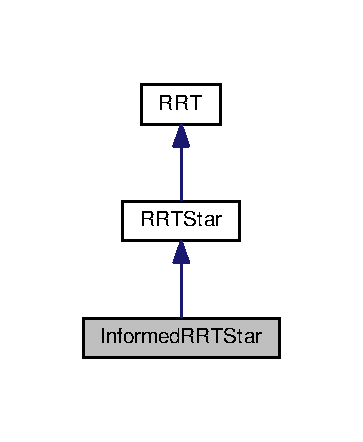
\includegraphics[width=174pt]{classInformedRRTStar__inherit__graph}
\end{center}
\end{figure}


Collaboration diagram for Informed\+R\+R\+T\+Star\+:
\nopagebreak
\begin{figure}[H]
\begin{center}
\leavevmode
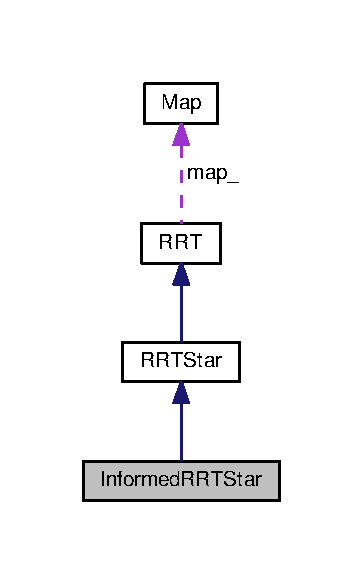
\includegraphics[width=174pt]{classInformedRRTStar__coll__graph}
\end{center}
\end{figure}
\subsection*{Public Member Functions}
\begin{DoxyCompactItemize}
\item 
\hyperlink{classInformedRRTStar_a4d5570b65e11a71d7ab132836eab25a5}{Informed\+R\+R\+T\+Star} ()
\begin{DoxyCompactList}\small\item\em Default constructor for Informed \hyperlink{classRRT}{R\+RT} Star. Prints basic information regarding planner. \end{DoxyCompactList}\item 
\hyperlink{classInformedRRTStar_a85971b0ff627946cb05f235e03b6a3f1}{$\sim$\+Informed\+R\+R\+T\+Star} ()
\begin{DoxyCompactList}\small\item\em Destructor for Informed \hyperlink{classRRT}{R\+RT} Star. \end{DoxyCompactList}\item 
std\+::vector$<$ double $>$ \hyperlink{classInformedRRTStar_a19d619bb1f106dbd36674a545e82a2b3}{generate\+Heuristic\+Node} ()
\begin{DoxyCompactList}\small\item\em samples a random point \mbox{[}x,y\mbox{]} in the heuristic region \end{DoxyCompactList}\item 
void \hyperlink{classInformedRRTStar_afbd7ccc52e9d6dfe734ffcb1bc386234}{run\+Planner} ()
\begin{DoxyCompactList}\small\item\em starts the execution of the Informed \hyperlink{classRRT}{R\+RT} Star planning algorithm \end{DoxyCompactList}\item 
void \hyperlink{classInformedRRTStar_ac13574a2c2a765599ef42283b069a471}{reset\+Planner} ()
\begin{DoxyCompactList}\small\item\em resets the planner by clearing all member varibles of Informed \hyperlink{classRRT}{R\+RT} Star class planner object \end{DoxyCompactList}\end{DoxyCompactItemize}
\subsection*{Additional Inherited Members}


\subsection{Detailed Description}
Class Informed \hyperlink{classRRT}{R\+RT} Star, derived from class \hyperlink{classRRT}{R\+RT} Star The following class \hyperlink{classRRT}{R\+RT} Star converges faster to find the optimized path found by \hyperlink{classRRT}{R\+RT} Star algorithm using a heuristic model. 

\subsection{Constructor \& Destructor Documentation}
\index{Informed\+R\+R\+T\+Star@{Informed\+R\+R\+T\+Star}!Informed\+R\+R\+T\+Star@{Informed\+R\+R\+T\+Star}}
\index{Informed\+R\+R\+T\+Star@{Informed\+R\+R\+T\+Star}!Informed\+R\+R\+T\+Star@{Informed\+R\+R\+T\+Star}}
\subsubsection[{\texorpdfstring{Informed\+R\+R\+T\+Star()}{InformedRRTStar()}}]{\setlength{\rightskip}{0pt plus 5cm}Informed\+R\+R\+T\+Star\+::\+Informed\+R\+R\+T\+Star (
\begin{DoxyParamCaption}
{}
\end{DoxyParamCaption}
)}\hypertarget{classInformedRRTStar_a4d5570b65e11a71d7ab132836eab25a5}{}\label{classInformedRRTStar_a4d5570b65e11a71d7ab132836eab25a5}


Default constructor for Informed \hyperlink{classRRT}{R\+RT} Star. Prints basic information regarding planner. 


\begin{DoxyParams}{Parameters}
{\em none} & \\
\hline
\end{DoxyParams}
\begin{DoxyReturn}{Returns}
void 
\end{DoxyReturn}
\index{Informed\+R\+R\+T\+Star@{Informed\+R\+R\+T\+Star}!````~Informed\+R\+R\+T\+Star@{$\sim$\+Informed\+R\+R\+T\+Star}}
\index{````~Informed\+R\+R\+T\+Star@{$\sim$\+Informed\+R\+R\+T\+Star}!Informed\+R\+R\+T\+Star@{Informed\+R\+R\+T\+Star}}
\subsubsection[{\texorpdfstring{$\sim$\+Informed\+R\+R\+T\+Star()}{~InformedRRTStar()}}]{\setlength{\rightskip}{0pt plus 5cm}Informed\+R\+R\+T\+Star\+::$\sim$\+Informed\+R\+R\+T\+Star (
\begin{DoxyParamCaption}
{}
\end{DoxyParamCaption}
)}\hypertarget{classInformedRRTStar_a85971b0ff627946cb05f235e03b6a3f1}{}\label{classInformedRRTStar_a85971b0ff627946cb05f235e03b6a3f1}


Destructor for Informed \hyperlink{classRRT}{R\+RT} Star. 


\begin{DoxyParams}{Parameters}
{\em none} & \\
\hline
\end{DoxyParams}
\begin{DoxyReturn}{Returns}
void 
\end{DoxyReturn}


\subsection{Member Function Documentation}
\index{Informed\+R\+R\+T\+Star@{Informed\+R\+R\+T\+Star}!generate\+Heuristic\+Node@{generate\+Heuristic\+Node}}
\index{generate\+Heuristic\+Node@{generate\+Heuristic\+Node}!Informed\+R\+R\+T\+Star@{Informed\+R\+R\+T\+Star}}
\subsubsection[{\texorpdfstring{generate\+Heuristic\+Node()}{generateHeuristicNode()}}]{\setlength{\rightskip}{0pt plus 5cm}std\+::vector$<$double$>$ Informed\+R\+R\+T\+Star\+::generate\+Heuristic\+Node (
\begin{DoxyParamCaption}
{}
\end{DoxyParamCaption}
)}\hypertarget{classInformedRRTStar_a19d619bb1f106dbd36674a545e82a2b3}{}\label{classInformedRRTStar_a19d619bb1f106dbd36674a545e82a2b3}


samples a random point \mbox{[}x,y\mbox{]} in the heuristic region 


\begin{DoxyParams}{Parameters}
{\em none} & \\
\hline
\end{DoxyParams}
\begin{DoxyReturn}{Returns}
vector \mbox{[}x,y\mbox{]} as double elements 
\end{DoxyReturn}
\index{Informed\+R\+R\+T\+Star@{Informed\+R\+R\+T\+Star}!reset\+Planner@{reset\+Planner}}
\index{reset\+Planner@{reset\+Planner}!Informed\+R\+R\+T\+Star@{Informed\+R\+R\+T\+Star}}
\subsubsection[{\texorpdfstring{reset\+Planner()}{resetPlanner()}}]{\setlength{\rightskip}{0pt plus 5cm}void Informed\+R\+R\+T\+Star\+::reset\+Planner (
\begin{DoxyParamCaption}
{}
\end{DoxyParamCaption}
)\hspace{0.3cm}{\ttfamily [virtual]}}\hypertarget{classInformedRRTStar_ac13574a2c2a765599ef42283b069a471}{}\label{classInformedRRTStar_ac13574a2c2a765599ef42283b069a471}


resets the planner by clearing all member varibles of Informed \hyperlink{classRRT}{R\+RT} Star class planner object 


\begin{DoxyParams}{Parameters}
{\em none} & \\
\hline
\end{DoxyParams}
\begin{DoxyReturn}{Returns}
void 
\end{DoxyReturn}


Reimplemented from \hyperlink{classRRTStar_a713736e18edd589d262dd4c2efc1e18d}{R\+R\+T\+Star}.

\index{Informed\+R\+R\+T\+Star@{Informed\+R\+R\+T\+Star}!run\+Planner@{run\+Planner}}
\index{run\+Planner@{run\+Planner}!Informed\+R\+R\+T\+Star@{Informed\+R\+R\+T\+Star}}
\subsubsection[{\texorpdfstring{run\+Planner()}{runPlanner()}}]{\setlength{\rightskip}{0pt plus 5cm}void Informed\+R\+R\+T\+Star\+::run\+Planner (
\begin{DoxyParamCaption}
{}
\end{DoxyParamCaption}
)\hspace{0.3cm}{\ttfamily [virtual]}}\hypertarget{classInformedRRTStar_afbd7ccc52e9d6dfe734ffcb1bc386234}{}\label{classInformedRRTStar_afbd7ccc52e9d6dfe734ffcb1bc386234}


starts the execution of the Informed \hyperlink{classRRT}{R\+RT} Star planning algorithm 


\begin{DoxyParams}{Parameters}
{\em none} & \\
\hline
\end{DoxyParams}
\begin{DoxyReturn}{Returns}
void 
\end{DoxyReturn}


Reimplemented from \hyperlink{classRRTStar_a5018db145f3a5bb5b4a13b710009ae55}{R\+R\+T\+Star}.



The documentation for this class was generated from the following file\+:\begin{DoxyCompactItemize}
\item 
/home/srinidhi/\+Git\+Hub/\+My Repos/\+E\+N\+P\+M808\+X-\/\+Midterm-\/\+Informed\+R\+R\+T\+Star/include/Informed\+R\+R\+T\+Star.\+hpp\end{DoxyCompactItemize}

\hypertarget{classMap}{}\section{Map Class Reference}
\label{classMap}\index{Map@{Map}}


Class \hyperlink{classMap}{Map} The following class \hyperlink{classMap}{Map} aids in storing the layout of the environment.  




{\ttfamily \#include $<$map.\+hpp$>$}

\subsection*{Public Member Functions}
\begin{DoxyCompactItemize}
\item 
\hyperlink{classMap_a0f5ad0fd4563497b4214038cbca8b582}{Map} ()
\begin{DoxyCompactList}\small\item\em Default constructor for \hyperlink{classMap}{Map}. \end{DoxyCompactList}\item 
\hyperlink{classMap_aa403fbe09394ccf39747588f5168e3b2}{$\sim$\+Map} ()
\begin{DoxyCompactList}\small\item\em Destructor for \hyperlink{classMap}{Map}. \end{DoxyCompactList}\item 
void \hyperlink{classMap_a86751846501ae330d05846a326d3e27b}{set\+Workspace\+Boundary} (const std\+::vector$<$ std\+::pair$<$ double, double $>$$>$ \&\hyperlink{MapTest_8cpp_ad2559d9d65caf07bc831e905bc151444}{boundary})
\begin{DoxyCompactList}\small\item\em setter function to set workspace boundary \end{DoxyCompactList}\item 
void \hyperlink{classMap_a0eba67299e0745bc6ef754634e79048d}{add\+Obstacle} (const std\+::vector$<$ double $>$ \&obstacle)
\begin{DoxyCompactList}\small\item\em function to add obstacle to a \hyperlink{classMap}{Map} \end{DoxyCompactList}\item 
bool \hyperlink{classMap_abf3c57ffaaee4b5c69a4db9cbae65f21}{on\+Segment} (const std\+::pair$<$ double, double $>$ \&first\+Point, const std\+::pair$<$ double, double $>$ \&second\+Point, const std\+::pair$<$ double, double $>$ \&third\+Point)
\begin{DoxyCompactList}\small\item\em checks if the second point lies on the line segment connecting first point and third point. \end{DoxyCompactList}\item 
int \hyperlink{classMap_ada38d0c2e965ac5c0ef5059e83fc4fb8}{get\+Orientation} (const std\+::pair$<$ double, double $>$ \&first\+Point, const std\+::pair$<$ double, double $>$ \&second\+Point, const std\+::pair$<$ double, double $>$ \&third\+Point)
\begin{DoxyCompactList}\small\item\em determines the oreintation i.\+e clockwise, anti-\/clockwise or collinearity of three ordered points. \end{DoxyCompactList}\item 
bool \hyperlink{classMap_ae48b43df43e2592d3813186f2fdec3c0}{is\+Intersect} (const std\+::pair$<$ double, double $>$ \&tree\+Node, const std\+::pair$<$ double, double $>$ \&new\+Node, const std\+::pair$<$ double, double $>$ \&first\+Vertex, const std\+::pair$<$ double, double $>$ \&second\+Vertex)
\begin{DoxyCompactList}\small\item\em determines if the line segments of tree node and new node, and first vertex and second vertex intersect \end{DoxyCompactList}\item 
bool \hyperlink{classMap_a310fd37abaf86fc980580fdbfcb592b8}{is\+Outof\+Map} (const std\+::pair$<$ double, double $>$ \&node)
\begin{DoxyCompactList}\small\item\em determines if the given node is out of map bounds \end{DoxyCompactList}\item 
bool \hyperlink{classMap_a4b6c14abb59b0e2bed63888271118723}{is\+Valid\+Node} (const std\+::pair$<$ double, double $>$ \&tree\+Node, const std\+::pair$<$ double, double $>$ \&new\+Node)
\begin{DoxyCompactList}\small\item\em determines if the given node can be added to the existing tree in the workspace without any conflicts \end{DoxyCompactList}\item 
void \hyperlink{classMap_a79a7d2715d8face71c5f16be9e14ac0a}{reset\+Map} ()
\begin{DoxyCompactList}\small\item\em function to reset the map by clearing the member variables \end{DoxyCompactList}\end{DoxyCompactItemize}
\subsection*{Public Attributes}
\begin{DoxyCompactItemize}
\item 
std\+::vector$<$ std\+::vector$<$ double $>$ $>$ \hyperlink{classMap_a8f459ed4a725e13ae680c26dfb4a77a3}{obstacle\+List}
\item 
std\+::vector$<$ std\+::pair$<$ double, double $>$ $>$ \hyperlink{classMap_ad93f26cfc04f6cf732a4f534765e57f7}{workspace\+Boundary}
\begin{DoxyCompactList}\small\item\em of paired points \mbox{[}x,y\mbox{]} \end{DoxyCompactList}\item 
std\+::vector$<$ double $>$ \hyperlink{classMap_a8b9bf67221211a1afa6cd05458f01e5a}{boundary\+Xlimits}
\item 
std\+::vector$<$ double $>$ \hyperlink{classMap_abbf6818140bc341cea9b30097a990d0a}{boundary\+Ylimits}
\end{DoxyCompactItemize}


\subsection{Detailed Description}
Class \hyperlink{classMap}{Map} The following class \hyperlink{classMap}{Map} aids in storing the layout of the environment. 

\subsection{Constructor \& Destructor Documentation}
\index{Map@{Map}!Map@{Map}}
\index{Map@{Map}!Map@{Map}}
\subsubsection[{\texorpdfstring{Map()}{Map()}}]{\setlength{\rightskip}{0pt plus 5cm}Map\+::\+Map (
\begin{DoxyParamCaption}
{}
\end{DoxyParamCaption}
)}\hypertarget{classMap_a0f5ad0fd4563497b4214038cbca8b582}{}\label{classMap_a0f5ad0fd4563497b4214038cbca8b582}


Default constructor for \hyperlink{classMap}{Map}. 


\begin{DoxyParams}{Parameters}
{\em none} & \\
\hline
\end{DoxyParams}
\begin{DoxyReturn}{Returns}
void 
\end{DoxyReturn}
\index{Map@{Map}!````~Map@{$\sim$\+Map}}
\index{````~Map@{$\sim$\+Map}!Map@{Map}}
\subsubsection[{\texorpdfstring{$\sim$\+Map()}{~Map()}}]{\setlength{\rightskip}{0pt plus 5cm}Map\+::$\sim$\+Map (
\begin{DoxyParamCaption}
{}
\end{DoxyParamCaption}
)}\hypertarget{classMap_aa403fbe09394ccf39747588f5168e3b2}{}\label{classMap_aa403fbe09394ccf39747588f5168e3b2}


Destructor for \hyperlink{classMap}{Map}. 


\begin{DoxyParams}{Parameters}
{\em none} & \\
\hline
\end{DoxyParams}
\begin{DoxyReturn}{Returns}
void 
\end{DoxyReturn}


\subsection{Member Function Documentation}
\index{Map@{Map}!add\+Obstacle@{add\+Obstacle}}
\index{add\+Obstacle@{add\+Obstacle}!Map@{Map}}
\subsubsection[{\texorpdfstring{add\+Obstacle(const std\+::vector$<$ double $>$ \&obstacle)}{addObstacle(const std::vector< double > &obstacle)}}]{\setlength{\rightskip}{0pt plus 5cm}void Map\+::add\+Obstacle (
\begin{DoxyParamCaption}
\item[{const std\+::vector$<$ double $>$ \&}]{obstacle}
\end{DoxyParamCaption}
)}\hypertarget{classMap_a0eba67299e0745bc6ef754634e79048d}{}\label{classMap_a0eba67299e0745bc6ef754634e79048d}


function to add obstacle to a \hyperlink{classMap}{Map} 


\begin{DoxyParams}{Parameters}
{\em obstacle} & is a vector of double points \mbox{[}x1,y1,x2,y2...xN,yN\mbox{]} defining the boundary vertices of an obstacle \\
\hline
\end{DoxyParams}
\begin{DoxyReturn}{Returns}
void 
\end{DoxyReturn}
\index{Map@{Map}!get\+Orientation@{get\+Orientation}}
\index{get\+Orientation@{get\+Orientation}!Map@{Map}}
\subsubsection[{\texorpdfstring{get\+Orientation(const std\+::pair$<$ double, double $>$ \&first\+Point, const std\+::pair$<$ double, double $>$ \&second\+Point, const std\+::pair$<$ double, double $>$ \&third\+Point)}{getOrientation(const std::pair< double, double > &firstPoint, const std::pair< double, double > &secondPoint, const std::pair< double, double > &thirdPoint)}}]{\setlength{\rightskip}{0pt plus 5cm}int Map\+::get\+Orientation (
\begin{DoxyParamCaption}
\item[{const std\+::pair$<$ double, double $>$ \&}]{first\+Point, }
\item[{const std\+::pair$<$ double, double $>$ \&}]{second\+Point, }
\item[{const std\+::pair$<$ double, double $>$ \&}]{third\+Point}
\end{DoxyParamCaption}
)}\hypertarget{classMap_ada38d0c2e965ac5c0ef5059e83fc4fb8}{}\label{classMap_ada38d0c2e965ac5c0ef5059e83fc4fb8}


determines the oreintation i.\+e clockwise, anti-\/clockwise or collinearity of three ordered points. 


\begin{DoxyParams}{Parameters}
{\em first\+Point,second\+Point} & and third\+Point are each pair of double \mbox{[}x,y\mbox{]} points in workspace \\
\hline
\end{DoxyParams}
\begin{DoxyReturn}{Returns}
0 if collinear, 1 if clockwise, 2 if anti-\/clockwise orientation as integer 
\end{DoxyReturn}
\index{Map@{Map}!is\+Intersect@{is\+Intersect}}
\index{is\+Intersect@{is\+Intersect}!Map@{Map}}
\subsubsection[{\texorpdfstring{is\+Intersect(const std\+::pair$<$ double, double $>$ \&tree\+Node, const std\+::pair$<$ double, double $>$ \&new\+Node, const std\+::pair$<$ double, double $>$ \&first\+Vertex, const std\+::pair$<$ double, double $>$ \&second\+Vertex)}{isIntersect(const std::pair< double, double > &treeNode, const std::pair< double, double > &newNode, const std::pair< double, double > &firstVertex, const std::pair< double, double > &secondVertex)}}]{\setlength{\rightskip}{0pt plus 5cm}bool Map\+::is\+Intersect (
\begin{DoxyParamCaption}
\item[{const std\+::pair$<$ double, double $>$ \&}]{tree\+Node, }
\item[{const std\+::pair$<$ double, double $>$ \&}]{new\+Node, }
\item[{const std\+::pair$<$ double, double $>$ \&}]{first\+Vertex, }
\item[{const std\+::pair$<$ double, double $>$ \&}]{second\+Vertex}
\end{DoxyParamCaption}
)}\hypertarget{classMap_ae48b43df43e2592d3813186f2fdec3c0}{}\label{classMap_ae48b43df43e2592d3813186f2fdec3c0}


determines if the line segments of tree node and new node, and first vertex and second vertex intersect 


\begin{DoxyParams}{Parameters}
{\em tree\+Node} & is the node in the tree as pair of double points \mbox{[}x,y\mbox{]} new\+Node is the node in the workspace as pair of double points \mbox{[}x,y\mbox{]} first\+Vertex, second\+Vertex are the vertices of an edge of an obstacle as pair of double points \mbox{[}x,y\mbox{]} each \\
\hline
\end{DoxyParams}
\begin{DoxyReturn}{Returns}
true if the line segments intersect, false if they don\textquotesingle{}t 
\end{DoxyReturn}
\index{Map@{Map}!is\+Outof\+Map@{is\+Outof\+Map}}
\index{is\+Outof\+Map@{is\+Outof\+Map}!Map@{Map}}
\subsubsection[{\texorpdfstring{is\+Outof\+Map(const std\+::pair$<$ double, double $>$ \&node)}{isOutofMap(const std::pair< double, double > &node)}}]{\setlength{\rightskip}{0pt plus 5cm}bool Map\+::is\+Outof\+Map (
\begin{DoxyParamCaption}
\item[{const std\+::pair$<$ double, double $>$ \&}]{node}
\end{DoxyParamCaption}
)}\hypertarget{classMap_a310fd37abaf86fc980580fdbfcb592b8}{}\label{classMap_a310fd37abaf86fc980580fdbfcb592b8}


determines if the given node is out of map bounds 


\begin{DoxyParams}{Parameters}
{\em node} & is the point \mbox{[}x,y\mbox{]} in workspace as pair of double \\
\hline
\end{DoxyParams}
\begin{DoxyReturn}{Returns}
true if node is out of boundary, false otherwise 
\end{DoxyReturn}
\index{Map@{Map}!is\+Valid\+Node@{is\+Valid\+Node}}
\index{is\+Valid\+Node@{is\+Valid\+Node}!Map@{Map}}
\subsubsection[{\texorpdfstring{is\+Valid\+Node(const std\+::pair$<$ double, double $>$ \&tree\+Node, const std\+::pair$<$ double, double $>$ \&new\+Node)}{isValidNode(const std::pair< double, double > &treeNode, const std::pair< double, double > &newNode)}}]{\setlength{\rightskip}{0pt plus 5cm}bool Map\+::is\+Valid\+Node (
\begin{DoxyParamCaption}
\item[{const std\+::pair$<$ double, double $>$ \&}]{tree\+Node, }
\item[{const std\+::pair$<$ double, double $>$ \&}]{new\+Node}
\end{DoxyParamCaption}
)}\hypertarget{classMap_a4b6c14abb59b0e2bed63888271118723}{}\label{classMap_a4b6c14abb59b0e2bed63888271118723}


determines if the given node can be added to the existing tree in the workspace without any conflicts 


\begin{DoxyParams}{Parameters}
{\em tree\+Node} & is the node in the tree as pair of double points \mbox{[}x,y\mbox{]} new\+Node is the node in the workspace as pair of double points \mbox{[}x,y\mbox{]} \\
\hline
\end{DoxyParams}
\begin{DoxyReturn}{Returns}
true if the tree\+Node can be added to the tree, false otherwise 
\end{DoxyReturn}
\index{Map@{Map}!on\+Segment@{on\+Segment}}
\index{on\+Segment@{on\+Segment}!Map@{Map}}
\subsubsection[{\texorpdfstring{on\+Segment(const std\+::pair$<$ double, double $>$ \&first\+Point, const std\+::pair$<$ double, double $>$ \&second\+Point, const std\+::pair$<$ double, double $>$ \&third\+Point)}{onSegment(const std::pair< double, double > &firstPoint, const std::pair< double, double > &secondPoint, const std::pair< double, double > &thirdPoint)}}]{\setlength{\rightskip}{0pt plus 5cm}bool Map\+::on\+Segment (
\begin{DoxyParamCaption}
\item[{const std\+::pair$<$ double, double $>$ \&}]{first\+Point, }
\item[{const std\+::pair$<$ double, double $>$ \&}]{second\+Point, }
\item[{const std\+::pair$<$ double, double $>$ \&}]{third\+Point}
\end{DoxyParamCaption}
)}\hypertarget{classMap_abf3c57ffaaee4b5c69a4db9cbae65f21}{}\label{classMap_abf3c57ffaaee4b5c69a4db9cbae65f21}


checks if the second point lies on the line segment connecting first point and third point. 


\begin{DoxyParams}{Parameters}
{\em first\+Point,second\+Point} & and third\+Point are each pair of double \mbox{[}x,y\mbox{]} points in workspace \\
\hline
\end{DoxyParams}
\begin{DoxyReturn}{Returns}
true if second point lies on the line segment, false if it doesn\textquotesingle{}t 
\end{DoxyReturn}
\index{Map@{Map}!reset\+Map@{reset\+Map}}
\index{reset\+Map@{reset\+Map}!Map@{Map}}
\subsubsection[{\texorpdfstring{reset\+Map()}{resetMap()}}]{\setlength{\rightskip}{0pt plus 5cm}void Map\+::reset\+Map (
\begin{DoxyParamCaption}
{}
\end{DoxyParamCaption}
)}\hypertarget{classMap_a79a7d2715d8face71c5f16be9e14ac0a}{}\label{classMap_a79a7d2715d8face71c5f16be9e14ac0a}


function to reset the map by clearing the member variables 


\begin{DoxyParams}{Parameters}
{\em none} & \\
\hline
\end{DoxyParams}
\begin{DoxyReturn}{Returns}
void 
\end{DoxyReturn}
\index{Map@{Map}!set\+Workspace\+Boundary@{set\+Workspace\+Boundary}}
\index{set\+Workspace\+Boundary@{set\+Workspace\+Boundary}!Map@{Map}}
\subsubsection[{\texorpdfstring{set\+Workspace\+Boundary(const std\+::vector$<$ std\+::pair$<$ double, double $>$$>$ \&boundary)}{setWorkspaceBoundary(const std::vector< std::pair< double, double >> &boundary)}}]{\setlength{\rightskip}{0pt plus 5cm}void Map\+::set\+Workspace\+Boundary (
\begin{DoxyParamCaption}
\item[{const std\+::vector$<$ std\+::pair$<$ double, double $>$$>$ \&}]{boundary}
\end{DoxyParamCaption}
)}\hypertarget{classMap_a86751846501ae330d05846a326d3e27b}{}\label{classMap_a86751846501ae330d05846a326d3e27b}


setter function to set workspace boundary 


\begin{DoxyParams}{Parameters}
{\em boundary} & is a vector of paired points \mbox{[}x,y\mbox{]} defining the boundary vertices \\
\hline
\end{DoxyParams}
\begin{DoxyReturn}{Returns}
void 
\end{DoxyReturn}


\subsection{Member Data Documentation}
\index{Map@{Map}!boundary\+Xlimits@{boundary\+Xlimits}}
\index{boundary\+Xlimits@{boundary\+Xlimits}!Map@{Map}}
\subsubsection[{\texorpdfstring{boundary\+Xlimits}{boundaryXlimits}}]{\setlength{\rightskip}{0pt plus 5cm}std\+::vector$<$double$>$ Map\+::boundary\+Xlimits}\hypertarget{classMap_a8b9bf67221211a1afa6cd05458f01e5a}{}\label{classMap_a8b9bf67221211a1afa6cd05458f01e5a}
Variable to hold min and max limits of the workspace boundary on x axis \index{Map@{Map}!boundary\+Ylimits@{boundary\+Ylimits}}
\index{boundary\+Ylimits@{boundary\+Ylimits}!Map@{Map}}
\subsubsection[{\texorpdfstring{boundary\+Ylimits}{boundaryYlimits}}]{\setlength{\rightskip}{0pt plus 5cm}std\+::vector$<$double$>$ Map\+::boundary\+Ylimits}\hypertarget{classMap_abbf6818140bc341cea9b30097a990d0a}{}\label{classMap_abbf6818140bc341cea9b30097a990d0a}
Variable to hold min and max limits of the workspace boundary on y axis \index{Map@{Map}!obstacle\+List@{obstacle\+List}}
\index{obstacle\+List@{obstacle\+List}!Map@{Map}}
\subsubsection[{\texorpdfstring{obstacle\+List}{obstacleList}}]{\setlength{\rightskip}{0pt plus 5cm}std\+::vector$<$std\+::vector$<$double$>$ $>$ Map\+::obstacle\+List}\hypertarget{classMap_a8f459ed4a725e13ae680c26dfb4a77a3}{}\label{classMap_a8f459ed4a725e13ae680c26dfb4a77a3}
Variable to hold list of obstacles. Each obstacle is defined as a vector of points in the order \mbox{[}x1, y1, x2, y2 ... xN, yN\mbox{]} \index{Map@{Map}!workspace\+Boundary@{workspace\+Boundary}}
\index{workspace\+Boundary@{workspace\+Boundary}!Map@{Map}}
\subsubsection[{\texorpdfstring{workspace\+Boundary}{workspaceBoundary}}]{\setlength{\rightskip}{0pt plus 5cm}std\+::vector$<$std\+::pair$<$double, double$>$ $>$ Map\+::workspace\+Boundary}\hypertarget{classMap_ad93f26cfc04f6cf732a4f534765e57f7}{}\label{classMap_ad93f26cfc04f6cf732a4f534765e57f7}


of paired points \mbox{[}x,y\mbox{]} 

Variable to hold workspace boundary as a vector 

The documentation for this class was generated from the following file\+:\begin{DoxyCompactItemize}
\item 
/home/srinidhi/\+Git\+Hub/\+My Repos/\+E\+N\+P\+M808\+X-\/\+Midterm-\/\+Informed\+R\+R\+T\+Star/include/\hyperlink{map_8hpp}{map.\+hpp}\end{DoxyCompactItemize}

\hypertarget{classRRT}{}\section{R\+RT Class Reference}
\label{classRRT}\index{R\+RT@{R\+RT}}


Class \hyperlink{classRRT}{R\+RT} The following class \hyperlink{classRRT}{R\+RT} implements the Rapidly-\/exploring random tree to find a path from start to goal in an environment.  




{\ttfamily \#include $<$R\+R\+T.\+hpp$>$}



Inheritance diagram for R\+RT\+:
\nopagebreak
\begin{figure}[H]
\begin{center}
\leavevmode
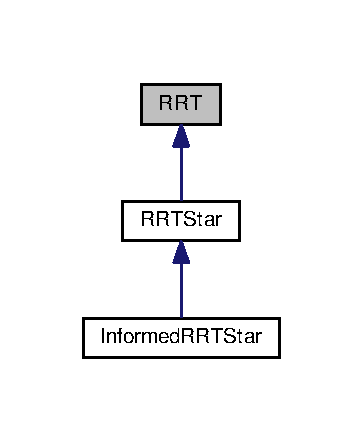
\includegraphics[width=174pt]{classRRT__inherit__graph}
\end{center}
\end{figure}


Collaboration diagram for R\+RT\+:
\nopagebreak
\begin{figure}[H]
\begin{center}
\leavevmode
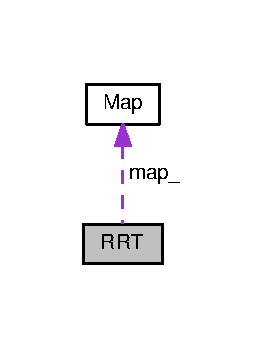
\includegraphics[width=127pt]{classRRT__coll__graph}
\end{center}
\end{figure}
\subsection*{Public Member Functions}
\begin{DoxyCompactItemize}
\item 
\hyperlink{classRRT_a0a7bb3a3af2d70c656764fbe8f6ae671}{R\+RT} ()
\begin{DoxyCompactList}\small\item\em Default constructor for \hyperlink{classRRT}{R\+RT}. Prints basic information regarding planner. \end{DoxyCompactList}\item 
\hyperlink{classRRT_ab16d13c231d664dddaf41f904d5770f8}{$\sim$\+R\+RT} ()
\begin{DoxyCompactList}\small\item\em Destructor for \hyperlink{classRRT}{R\+RT}. \end{DoxyCompactList}\item 
std\+::pair$<$ size\+\_\+t, double $>$ \hyperlink{classRRT_af036e6c57778da5d017493ee1a2d0d37}{get\+Planner\+Parameters} ()
\begin{DoxyCompactList}\small\item\em function to return planner parameters \end{DoxyCompactList}\item 
void \hyperlink{classRRT_a99d47b882000b264f594b374b18c49c0}{set\+Map} (const std\+::vector$<$ std\+::pair$<$ double, double $>$$>$ \&\hyperlink{MapTest_8cpp_ad2559d9d65caf07bc831e905bc151444}{boundary}, const std\+::vector$<$ std\+::vector$<$ double $>$$>$ \&\hyperlink{MapTest_8cpp_ab66426f62219d5ce7554221a370691fe}{obstacles})
\begin{DoxyCompactList}\small\item\em setter function to define the environment \end{DoxyCompactList}\item 
virtual void \hyperlink{classRRT_a4954f750e5aedfea24fb52771bd5b1af}{set\+Start\+And\+Goal} (const std\+::vector$<$ double $>$ \&start, const std\+::vector$<$ double $>$ \&goal)
\begin{DoxyCompactList}\small\item\em setter function to set start and goal point for the \hyperlink{classRRT}{R\+RT} algorithm \end{DoxyCompactList}\item 
std\+::vector$<$ double $>$ \hyperlink{classRRT_ab85d824e85c9c0e7ed5ee385f5649993}{generate\+Random\+Node} ()
\begin{DoxyCompactList}\small\item\em samples a random point \mbox{[}x,y\mbox{]} in the map environment \end{DoxyCompactList}\item 
double \hyperlink{classRRT_a71746e00550593ba81eff895a736bc83}{get\+Euclidean\+Distance} (const std\+::vector$<$ double $>$ \&node, const std\+::vector$<$ double $>$ \&tree\+Node)
\begin{DoxyCompactList}\small\item\em calculates the euclidean distance between a point and a R\+R\+Tree node \end{DoxyCompactList}\item 
virtual std\+::shared\+\_\+ptr$<$ \hyperlink{classRRTNode}{R\+R\+T\+Node} $>$ \hyperlink{classRRT_ae581ca8e7858e75e3958596f9dd57390}{find\+Closest\+Tree\+Node} (const std\+::vector$<$ double $>$ \&random\+Node)
\begin{DoxyCompactList}\small\item\em finds the closest node in the tree to a given randomly sampled node in the environment \end{DoxyCompactList}\item 
std\+::vector$<$ double $>$ \hyperlink{classRRT_a819276861e55d3c472c19dd92f4e6d58}{generate\+New\+Node} (const std\+::vector$<$ double $>$ \&random\+Node, const std\+::shared\+\_\+ptr$<$ \hyperlink{classRRTNode}{R\+R\+T\+Node} $>$ \&closest\+Tree\+Node)
\begin{DoxyCompactList}\small\item\em generates a new node that is reachable from the closest tree node to the randomly sampled node, at a drive/steer distance \end{DoxyCompactList}\item 
virtual void \hyperlink{classRRT_a2629b145454f54cca6a1ad796c27e900}{append\+R\+R\+Tree} (const std\+::vector$<$ double $>$ \&valid\+Node, const std\+::shared\+\_\+ptr$<$ \hyperlink{classRRTNode}{R\+R\+T\+Node} $>$ \&valid\+Node\+Parent)
\begin{DoxyCompactList}\small\item\em appends the R\+R\+Tree in the workspace with the new valid node \end{DoxyCompactList}\item 
bool \hyperlink{classRRT_ae952a5270a03a0dfe49ca110a6a430b7}{is\+Goal\+Reached} (const std\+::vector$<$ double $>$ \&new\+Node)
\begin{DoxyCompactList}\small\item\em checks if the goal node is within drivable distance from the current tree in the environment \end{DoxyCompactList}\item 
virtual std\+::vector$<$ std\+::pair$<$ double, double $>$ $>$ \hyperlink{classRRT_a35e29366864cebacda5cd52c1febaa73}{get\+Planner\+Path} ()
\begin{DoxyCompactList}\small\item\em returns a path found by the \hyperlink{classRRT}{R\+RT} algorithm as a set of waypoints \end{DoxyCompactList}\item 
std\+::vector$<$ \hyperlink{classRRTNode}{R\+R\+T\+Node} $>$ \hyperlink{classRRT_aba9e08111e7b76cd72acf2d0d4d560ae}{get\+R\+R\+Tree} ()
\begin{DoxyCompactList}\small\item\em returns the tree resulting from the \hyperlink{classRRT}{R\+RT} algorithm \end{DoxyCompactList}\item 
virtual void \hyperlink{classRRT_a57a214360eb86fc63d7300bc1ea94fde}{run\+Planner} ()
\begin{DoxyCompactList}\small\item\em starts the execution of the \hyperlink{classRRT}{R\+RT} planning algorithm \end{DoxyCompactList}\item 
virtual void \hyperlink{classRRT_a952ef4be01547b013ce5c64d912fe680}{reset\+Planner} ()
\begin{DoxyCompactList}\small\item\em resets the planner by clearing all member varibles of \hyperlink{classRRT}{R\+RT} class planner object \end{DoxyCompactList}\end{DoxyCompactItemize}
\subsection*{Public Attributes}
\begin{DoxyCompactItemize}
\item 
std\+::vector$<$ double $>$ \hyperlink{classRRT_a97431b141ce0849f645625c1be1ac198}{start\+Node\+\_\+}\hypertarget{classRRT_a97431b141ce0849f645625c1be1ac198}{}\label{classRRT_a97431b141ce0849f645625c1be1ac198}

\begin{DoxyCompactList}\small\item\em variable to hold the starting node for the algorithm \end{DoxyCompactList}\item 
std\+::vector$<$ double $>$ \hyperlink{classRRT_a01f224deb0e405704d56735301dca404}{goal\+Node\+\_\+}
\item 
\hyperlink{classMap}{Map} \hyperlink{classRRT_a534fd15ee26c5680a17ee3528a9e9b20}{map\+\_\+}
\end{DoxyCompactItemize}


\subsection{Detailed Description}
Class \hyperlink{classRRT}{R\+RT} The following class \hyperlink{classRRT}{R\+RT} implements the Rapidly-\/exploring random tree to find a path from start to goal in an environment. 

\subsection{Constructor \& Destructor Documentation}
\index{R\+RT@{R\+RT}!R\+RT@{R\+RT}}
\index{R\+RT@{R\+RT}!R\+RT@{R\+RT}}
\subsubsection[{\texorpdfstring{R\+R\+T()}{RRT()}}]{\setlength{\rightskip}{0pt plus 5cm}R\+R\+T\+::\+R\+RT (
\begin{DoxyParamCaption}
{}
\end{DoxyParamCaption}
)}\hypertarget{classRRT_a0a7bb3a3af2d70c656764fbe8f6ae671}{}\label{classRRT_a0a7bb3a3af2d70c656764fbe8f6ae671}


Default constructor for \hyperlink{classRRT}{R\+RT}. Prints basic information regarding planner. 


\begin{DoxyParams}{Parameters}
{\em none} & \\
\hline
\end{DoxyParams}
\begin{DoxyReturn}{Returns}
void 
\end{DoxyReturn}
\index{R\+RT@{R\+RT}!````~R\+RT@{$\sim$\+R\+RT}}
\index{````~R\+RT@{$\sim$\+R\+RT}!R\+RT@{R\+RT}}
\subsubsection[{\texorpdfstring{$\sim$\+R\+R\+T()}{~RRT()}}]{\setlength{\rightskip}{0pt plus 5cm}R\+R\+T\+::$\sim$\+R\+RT (
\begin{DoxyParamCaption}
{}
\end{DoxyParamCaption}
)}\hypertarget{classRRT_ab16d13c231d664dddaf41f904d5770f8}{}\label{classRRT_ab16d13c231d664dddaf41f904d5770f8}


Destructor for \hyperlink{classRRT}{R\+RT}. 


\begin{DoxyParams}{Parameters}
{\em none} & \\
\hline
\end{DoxyParams}
\begin{DoxyReturn}{Returns}
void 
\end{DoxyReturn}


\subsection{Member Function Documentation}
\index{R\+RT@{R\+RT}!append\+R\+R\+Tree@{append\+R\+R\+Tree}}
\index{append\+R\+R\+Tree@{append\+R\+R\+Tree}!R\+RT@{R\+RT}}
\subsubsection[{\texorpdfstring{append\+R\+R\+Tree(const std\+::vector$<$ double $>$ \&valid\+Node, const std\+::shared\+\_\+ptr$<$ R\+R\+T\+Node $>$ \&valid\+Node\+Parent)}{appendRRTree(const std::vector< double > &validNode, const std::shared_ptr< RRTNode > &validNodeParent)}}]{\setlength{\rightskip}{0pt plus 5cm}virtual void R\+R\+T\+::append\+R\+R\+Tree (
\begin{DoxyParamCaption}
\item[{const std\+::vector$<$ double $>$ \&}]{valid\+Node, }
\item[{const std\+::shared\+\_\+ptr$<$ {\bf R\+R\+T\+Node} $>$ \&}]{valid\+Node\+Parent}
\end{DoxyParamCaption}
)\hspace{0.3cm}{\ttfamily [virtual]}}\hypertarget{classRRT_a2629b145454f54cca6a1ad796c27e900}{}\label{classRRT_a2629b145454f54cca6a1ad796c27e900}


appends the R\+R\+Tree in the workspace with the new valid node 


\begin{DoxyParams}{Parameters}
{\em valid\+Node} & is the newly generated node at a drivable distance to the current tree in the environment as a vector of double elements \mbox{[}x,y\mbox{]} valid\+Node\+Parent is the pointer to the object of class \hyperlink{classRRT}{R\+RT} pointing to the parent of the valid\+Node \\
\hline
\end{DoxyParams}
\begin{DoxyReturn}{Returns}
void 
\end{DoxyReturn}


Reimplemented in \hyperlink{classRRTStar_a3b1f7e66c99881faa190034b0ff2b101}{R\+R\+T\+Star}.

\index{R\+RT@{R\+RT}!find\+Closest\+Tree\+Node@{find\+Closest\+Tree\+Node}}
\index{find\+Closest\+Tree\+Node@{find\+Closest\+Tree\+Node}!R\+RT@{R\+RT}}
\subsubsection[{\texorpdfstring{find\+Closest\+Tree\+Node(const std\+::vector$<$ double $>$ \&random\+Node)}{findClosestTreeNode(const std::vector< double > &randomNode)}}]{\setlength{\rightskip}{0pt plus 5cm}virtual std\+::shared\+\_\+ptr$<${\bf R\+R\+T\+Node}$>$ R\+R\+T\+::find\+Closest\+Tree\+Node (
\begin{DoxyParamCaption}
\item[{const std\+::vector$<$ double $>$ \&}]{random\+Node}
\end{DoxyParamCaption}
)\hspace{0.3cm}{\ttfamily [virtual]}}\hypertarget{classRRT_ae581ca8e7858e75e3958596f9dd57390}{}\label{classRRT_ae581ca8e7858e75e3958596f9dd57390}


finds the closest node in the tree to a given randomly sampled node in the environment 


\begin{DoxyParams}{Parameters}
{\em random\+Node} & is the randomly sampled node in the environment as a vector of double elements \\
\hline
\end{DoxyParams}
\begin{DoxyReturn}{Returns}
A smart pointer (shared\+\_\+ptr) pointing to the object of the closest tree node 
\end{DoxyReturn}


Reimplemented in \hyperlink{classRRTStar_ac8825e6654bc43d7d82918451e09ea89}{R\+R\+T\+Star}.

\index{R\+RT@{R\+RT}!generate\+New\+Node@{generate\+New\+Node}}
\index{generate\+New\+Node@{generate\+New\+Node}!R\+RT@{R\+RT}}
\subsubsection[{\texorpdfstring{generate\+New\+Node(const std\+::vector$<$ double $>$ \&random\+Node, const std\+::shared\+\_\+ptr$<$ R\+R\+T\+Node $>$ \&closest\+Tree\+Node)}{generateNewNode(const std::vector< double > &randomNode, const std::shared_ptr< RRTNode > &closestTreeNode)}}]{\setlength{\rightskip}{0pt plus 5cm}std\+::vector$<$double$>$ R\+R\+T\+::generate\+New\+Node (
\begin{DoxyParamCaption}
\item[{const std\+::vector$<$ double $>$ \&}]{random\+Node, }
\item[{const std\+::shared\+\_\+ptr$<$ {\bf R\+R\+T\+Node} $>$ \&}]{closest\+Tree\+Node}
\end{DoxyParamCaption}
)}\hypertarget{classRRT_a819276861e55d3c472c19dd92f4e6d58}{}\label{classRRT_a819276861e55d3c472c19dd92f4e6d58}


generates a new node that is reachable from the closest tree node to the randomly sampled node, at a drive/steer distance 


\begin{DoxyParams}{Parameters}
{\em random\+Node} & is the randomly sampled node in the environment as a vector of double elements \mbox{[}x,y\mbox{]} closest\+Tree\+Node is a pointer to the object of class \hyperlink{classRRT}{R\+RT} representing the closest node in the tree to the random node \\
\hline
\end{DoxyParams}
\begin{DoxyReturn}{Returns}
a vector of double elements representing the new node \mbox{[}x,y\mbox{]} drivable from the tree node 
\end{DoxyReturn}
\index{R\+RT@{R\+RT}!generate\+Random\+Node@{generate\+Random\+Node}}
\index{generate\+Random\+Node@{generate\+Random\+Node}!R\+RT@{R\+RT}}
\subsubsection[{\texorpdfstring{generate\+Random\+Node()}{generateRandomNode()}}]{\setlength{\rightskip}{0pt plus 5cm}std\+::vector$<$double$>$ R\+R\+T\+::generate\+Random\+Node (
\begin{DoxyParamCaption}
{}
\end{DoxyParamCaption}
)}\hypertarget{classRRT_ab85d824e85c9c0e7ed5ee385f5649993}{}\label{classRRT_ab85d824e85c9c0e7ed5ee385f5649993}


samples a random point \mbox{[}x,y\mbox{]} in the map environment 


\begin{DoxyParams}{Parameters}
{\em none} & \\
\hline
\end{DoxyParams}
\begin{DoxyReturn}{Returns}
vector \mbox{[}x,y\mbox{]} as double elements 
\end{DoxyReturn}
\index{R\+RT@{R\+RT}!get\+Euclidean\+Distance@{get\+Euclidean\+Distance}}
\index{get\+Euclidean\+Distance@{get\+Euclidean\+Distance}!R\+RT@{R\+RT}}
\subsubsection[{\texorpdfstring{get\+Euclidean\+Distance(const std\+::vector$<$ double $>$ \&node, const std\+::vector$<$ double $>$ \&tree\+Node)}{getEuclideanDistance(const std::vector< double > &node, const std::vector< double > &treeNode)}}]{\setlength{\rightskip}{0pt plus 5cm}double R\+R\+T\+::get\+Euclidean\+Distance (
\begin{DoxyParamCaption}
\item[{const std\+::vector$<$ double $>$ \&}]{node, }
\item[{const std\+::vector$<$ double $>$ \&}]{tree\+Node}
\end{DoxyParamCaption}
)}\hypertarget{classRRT_a71746e00550593ba81eff895a736bc83}{}\label{classRRT_a71746e00550593ba81eff895a736bc83}


calculates the euclidean distance between a point and a R\+R\+Tree node 


\begin{DoxyParams}{Parameters}
{\em node} & is a random point in the environment as a vector of double points tree\+Node is a vector of double type representing a node in the R\+R\+Tree \\
\hline
\end{DoxyParams}
\begin{DoxyReturn}{Returns}
the euclidean distance between the random node and the tree node as double element 
\end{DoxyReturn}
\index{R\+RT@{R\+RT}!get\+Planner\+Parameters@{get\+Planner\+Parameters}}
\index{get\+Planner\+Parameters@{get\+Planner\+Parameters}!R\+RT@{R\+RT}}
\subsubsection[{\texorpdfstring{get\+Planner\+Parameters()}{getPlannerParameters()}}]{\setlength{\rightskip}{0pt plus 5cm}std\+::pair$<$size\+\_\+t, double$>$ R\+R\+T\+::get\+Planner\+Parameters (
\begin{DoxyParamCaption}
{}
\end{DoxyParamCaption}
)}\hypertarget{classRRT_af036e6c57778da5d017493ee1a2d0d37}{}\label{classRRT_af036e6c57778da5d017493ee1a2d0d37}


function to return planner parameters 


\begin{DoxyParams}{Parameters}
{\em none} & \\
\hline
\end{DoxyParams}
\begin{DoxyReturn}{Returns}
pair of values (unsigned int, double) defining the max iterations and drive paramater respectively 
\end{DoxyReturn}
\index{R\+RT@{R\+RT}!get\+Planner\+Path@{get\+Planner\+Path}}
\index{get\+Planner\+Path@{get\+Planner\+Path}!R\+RT@{R\+RT}}
\subsubsection[{\texorpdfstring{get\+Planner\+Path()}{getPlannerPath()}}]{\setlength{\rightskip}{0pt plus 5cm}virtual std\+::vector$<$std\+::pair$<$double, double$>$ $>$ R\+R\+T\+::get\+Planner\+Path (
\begin{DoxyParamCaption}
{}
\end{DoxyParamCaption}
)\hspace{0.3cm}{\ttfamily [virtual]}}\hypertarget{classRRT_a35e29366864cebacda5cd52c1febaa73}{}\label{classRRT_a35e29366864cebacda5cd52c1febaa73}


returns a path found by the \hyperlink{classRRT}{R\+RT} algorithm as a set of waypoints 


\begin{DoxyParams}{Parameters}
{\em none} & \\
\hline
\end{DoxyParams}
\begin{DoxyReturn}{Returns}
vector of pair of double elements \mbox{[}x,y\mbox{]} representing the set of waypoints 
\end{DoxyReturn}


Reimplemented in \hyperlink{classRRTStar_a9d415973b5fbafa4435203fb56ac3357}{R\+R\+T\+Star}.

\index{R\+RT@{R\+RT}!get\+R\+R\+Tree@{get\+R\+R\+Tree}}
\index{get\+R\+R\+Tree@{get\+R\+R\+Tree}!R\+RT@{R\+RT}}
\subsubsection[{\texorpdfstring{get\+R\+R\+Tree()}{getRRTree()}}]{\setlength{\rightskip}{0pt plus 5cm}std\+::vector$<${\bf R\+R\+T\+Node}$>$ R\+R\+T\+::get\+R\+R\+Tree (
\begin{DoxyParamCaption}
{}
\end{DoxyParamCaption}
)}\hypertarget{classRRT_aba9e08111e7b76cd72acf2d0d4d560ae}{}\label{classRRT_aba9e08111e7b76cd72acf2d0d4d560ae}


returns the tree resulting from the \hyperlink{classRRT}{R\+RT} algorithm 


\begin{DoxyParams}{Parameters}
{\em none} & \\
\hline
\end{DoxyParams}
\begin{DoxyReturn}{Returns}
vector of nodes i.\+e objects of \hyperlink{classRRTNode}{R\+R\+T\+Node} class 
\end{DoxyReturn}
\index{R\+RT@{R\+RT}!is\+Goal\+Reached@{is\+Goal\+Reached}}
\index{is\+Goal\+Reached@{is\+Goal\+Reached}!R\+RT@{R\+RT}}
\subsubsection[{\texorpdfstring{is\+Goal\+Reached(const std\+::vector$<$ double $>$ \&new\+Node)}{isGoalReached(const std::vector< double > &newNode)}}]{\setlength{\rightskip}{0pt plus 5cm}bool R\+R\+T\+::is\+Goal\+Reached (
\begin{DoxyParamCaption}
\item[{const std\+::vector$<$ double $>$ \&}]{new\+Node}
\end{DoxyParamCaption}
)}\hypertarget{classRRT_ae952a5270a03a0dfe49ca110a6a430b7}{}\label{classRRT_ae952a5270a03a0dfe49ca110a6a430b7}


checks if the goal node is within drivable distance from the current tree in the environment 


\begin{DoxyParams}{Parameters}
{\em new\+Node} & is the latest node added to the R\+R\+Tree as a vector of double elements \mbox{[}x,y\mbox{]} \\
\hline
\end{DoxyParams}
\begin{DoxyReturn}{Returns}
true if goal is within drivable range, false otherwise 
\end{DoxyReturn}
\index{R\+RT@{R\+RT}!reset\+Planner@{reset\+Planner}}
\index{reset\+Planner@{reset\+Planner}!R\+RT@{R\+RT}}
\subsubsection[{\texorpdfstring{reset\+Planner()}{resetPlanner()}}]{\setlength{\rightskip}{0pt plus 5cm}virtual void R\+R\+T\+::reset\+Planner (
\begin{DoxyParamCaption}
{}
\end{DoxyParamCaption}
)\hspace{0.3cm}{\ttfamily [virtual]}}\hypertarget{classRRT_a952ef4be01547b013ce5c64d912fe680}{}\label{classRRT_a952ef4be01547b013ce5c64d912fe680}


resets the planner by clearing all member varibles of \hyperlink{classRRT}{R\+RT} class planner object 


\begin{DoxyParams}{Parameters}
{\em none} & \\
\hline
\end{DoxyParams}
\begin{DoxyReturn}{Returns}
void 
\end{DoxyReturn}


Reimplemented in \hyperlink{classRRTStar_a713736e18edd589d262dd4c2efc1e18d}{R\+R\+T\+Star}, and \hyperlink{classInformedRRTStar_ac13574a2c2a765599ef42283b069a471}{Informed\+R\+R\+T\+Star}.

\index{R\+RT@{R\+RT}!run\+Planner@{run\+Planner}}
\index{run\+Planner@{run\+Planner}!R\+RT@{R\+RT}}
\subsubsection[{\texorpdfstring{run\+Planner()}{runPlanner()}}]{\setlength{\rightskip}{0pt plus 5cm}virtual void R\+R\+T\+::run\+Planner (
\begin{DoxyParamCaption}
{}
\end{DoxyParamCaption}
)\hspace{0.3cm}{\ttfamily [virtual]}}\hypertarget{classRRT_a57a214360eb86fc63d7300bc1ea94fde}{}\label{classRRT_a57a214360eb86fc63d7300bc1ea94fde}


starts the execution of the \hyperlink{classRRT}{R\+RT} planning algorithm 


\begin{DoxyParams}{Parameters}
{\em none} & \\
\hline
\end{DoxyParams}
\begin{DoxyReturn}{Returns}
void 
\end{DoxyReturn}


Reimplemented in \hyperlink{classRRTStar_a5018db145f3a5bb5b4a13b710009ae55}{R\+R\+T\+Star}, and \hyperlink{classInformedRRTStar_afbd7ccc52e9d6dfe734ffcb1bc386234}{Informed\+R\+R\+T\+Star}.

\index{R\+RT@{R\+RT}!set\+Map@{set\+Map}}
\index{set\+Map@{set\+Map}!R\+RT@{R\+RT}}
\subsubsection[{\texorpdfstring{set\+Map(const std\+::vector$<$ std\+::pair$<$ double, double $>$$>$ \&boundary, const std\+::vector$<$ std\+::vector$<$ double $>$$>$ \&obstacles)}{setMap(const std::vector< std::pair< double, double >> &boundary, const std::vector< std::vector< double >> &obstacles)}}]{\setlength{\rightskip}{0pt plus 5cm}void R\+R\+T\+::set\+Map (
\begin{DoxyParamCaption}
\item[{const std\+::vector$<$ std\+::pair$<$ double, double $>$$>$ \&}]{boundary, }
\item[{const std\+::vector$<$ std\+::vector$<$ double $>$$>$ \&}]{obstacles}
\end{DoxyParamCaption}
)}\hypertarget{classRRT_a99d47b882000b264f594b374b18c49c0}{}\label{classRRT_a99d47b882000b264f594b374b18c49c0}


setter function to define the environment 


\begin{DoxyParams}{Parameters}
{\em boundary} & is a vector of paired points \mbox{[}x,y\mbox{]} defining the boundary vertices. obstacles is a vector of obstacle container which in turn is a vector of double points \mbox{[}x1,y1,x2,y2...xN,yN\mbox{]} defining the boundary vertices of an obstacle in the environment. \\
\hline
\end{DoxyParams}
\begin{DoxyReturn}{Returns}
void 
\end{DoxyReturn}
\index{R\+RT@{R\+RT}!set\+Start\+And\+Goal@{set\+Start\+And\+Goal}}
\index{set\+Start\+And\+Goal@{set\+Start\+And\+Goal}!R\+RT@{R\+RT}}
\subsubsection[{\texorpdfstring{set\+Start\+And\+Goal(const std\+::vector$<$ double $>$ \&start, const std\+::vector$<$ double $>$ \&goal)}{setStartAndGoal(const std::vector< double > &start, const std::vector< double > &goal)}}]{\setlength{\rightskip}{0pt plus 5cm}virtual void R\+R\+T\+::set\+Start\+And\+Goal (
\begin{DoxyParamCaption}
\item[{const std\+::vector$<$ double $>$ \&}]{start, }
\item[{const std\+::vector$<$ double $>$ \&}]{goal}
\end{DoxyParamCaption}
)\hspace{0.3cm}{\ttfamily [virtual]}}\hypertarget{classRRT_a4954f750e5aedfea24fb52771bd5b1af}{}\label{classRRT_a4954f750e5aedfea24fb52771bd5b1af}


setter function to set start and goal point for the \hyperlink{classRRT}{R\+RT} algorithm 


\begin{DoxyParams}{Parameters}
{\em start} & defines the start point as a vector \mbox{[}x,y\mbox{]} of double elements goal defines the goal point as a vector \mbox{[}x,y\mbox{]} of double elements \\
\hline
\end{DoxyParams}
\begin{DoxyReturn}{Returns}
void 
\end{DoxyReturn}


Reimplemented in \hyperlink{classRRTStar_a1205f9b17419186be4a575151e68f304}{R\+R\+T\+Star}.



\subsection{Member Data Documentation}
\index{R\+RT@{R\+RT}!goal\+Node\+\_\+@{goal\+Node\+\_\+}}
\index{goal\+Node\+\_\+@{goal\+Node\+\_\+}!R\+RT@{R\+RT}}
\subsubsection[{\texorpdfstring{goal\+Node\+\_\+}{goalNode_}}]{\setlength{\rightskip}{0pt plus 5cm}std\+::vector$<$double$>$ R\+R\+T\+::goal\+Node\+\_\+}\hypertarget{classRRT_a01f224deb0e405704d56735301dca404}{}\label{classRRT_a01f224deb0e405704d56735301dca404}
variable to hold the goal node where the algorithm terminates \index{R\+RT@{R\+RT}!map\+\_\+@{map\+\_\+}}
\index{map\+\_\+@{map\+\_\+}!R\+RT@{R\+RT}}
\subsubsection[{\texorpdfstring{map\+\_\+}{map_}}]{\setlength{\rightskip}{0pt plus 5cm}{\bf Map} R\+R\+T\+::map\+\_\+}\hypertarget{classRRT_a534fd15ee26c5680a17ee3528a9e9b20}{}\label{classRRT_a534fd15ee26c5680a17ee3528a9e9b20}
object of class \hyperlink{classMap}{Map} to hold the information regarding the environment 

The documentation for this class was generated from the following file\+:\begin{DoxyCompactItemize}
\item 
/home/srinidhi/\+Git\+Hub/\+My Repos/\+E\+N\+P\+M808\+X-\/\+Midterm-\/\+Informed\+R\+R\+T\+Star/include/\hyperlink{RRT_8hpp}{R\+R\+T.\+hpp}\end{DoxyCompactItemize}

\hypertarget{classRRTNode}{}\section{R\+R\+T\+Node Class Reference}
\label{classRRTNode}\index{R\+R\+T\+Node@{R\+R\+T\+Node}}


Class \hyperlink{classRRTNode}{R\+R\+T\+Node} The following class \hyperlink{classRRTNode}{R\+R\+T\+Node} is used to hold information of a node in the tree formed by \hyperlink{classRRT}{R\+RT} algorithm.  




{\ttfamily \#include $<$R\+R\+T\+Node.\+hpp$>$}

\subsection*{Public Member Functions}
\begin{DoxyCompactItemize}
\item 
\hyperlink{classRRTNode_a450dfa8045c8da49f359790501878106}{R\+R\+T\+Node} ()
\begin{DoxyCompactList}\small\item\em Default constructor for \hyperlink{classRRTNode}{R\+R\+T\+Node}. \end{DoxyCompactList}\item 
\hyperlink{classRRTNode_a6809e4173f614885337cb9e0f1ab3222}{$\sim$\+R\+R\+T\+Node} ()
\begin{DoxyCompactList}\small\item\em Destructor for \hyperlink{classRRTNode}{R\+R\+T\+Node}. \end{DoxyCompactList}\item 
void \hyperlink{classRRTNode_ab1a5aa8a8e7c33fca0cee09c208a2b51}{set\+State} (const double \&x, const double \&y)
\begin{DoxyCompactList}\small\item\em setter function to set state \mbox{[}x,y\mbox{]} of the node \end{DoxyCompactList}\item 
std\+::vector$<$ double $>$ \hyperlink{classRRTNode_a73f2b83a8babef45d6336cd512532257}{get\+State} ()
\begin{DoxyCompactList}\small\item\em function to return state \mbox{[}x,y\mbox{]} of the node \end{DoxyCompactList}\item 
void \hyperlink{classRRTNode_a168d651956a9d3ff5a97dfc14b2cbff9}{set\+Parent} (const std\+::shared\+\_\+ptr$<$ \hyperlink{classRRTNode}{R\+R\+T\+Node} $>$ \&parent\+Object)
\begin{DoxyCompactList}\small\item\em setter function to set parent node of the current node \end{DoxyCompactList}\item 
std\+::shared\+\_\+ptr$<$ \hyperlink{classRRTNode}{R\+R\+T\+Node} $>$ \hyperlink{classRRTNode_ad53ba7bac9b3119510b6a7b5dc3ac378}{get\+Parent} ()
\begin{DoxyCompactList}\small\item\em function to return current node\textquotesingle{}s parent node object pointer \end{DoxyCompactList}\item 
void \hyperlink{classRRTNode_af7986ea058b3a697bf1977903b286edd}{set\+Cost\+To\+Come} (const double \&cost)
\begin{DoxyCompactList}\small\item\em setter function to set cost to come for the node \end{DoxyCompactList}\item 
double \hyperlink{classRRTNode_aef17b4bd6901c1b1bfc381f862ebfaa1}{get\+Cost\+To\+Come} ()
\begin{DoxyCompactList}\small\item\em function to return cost to come of the node \end{DoxyCompactList}\end{DoxyCompactItemize}


\subsection{Detailed Description}
Class \hyperlink{classRRTNode}{R\+R\+T\+Node} The following class \hyperlink{classRRTNode}{R\+R\+T\+Node} is used to hold information of a node in the tree formed by \hyperlink{classRRT}{R\+RT} algorithm. 

\subsection{Constructor \& Destructor Documentation}
\index{R\+R\+T\+Node@{R\+R\+T\+Node}!R\+R\+T\+Node@{R\+R\+T\+Node}}
\index{R\+R\+T\+Node@{R\+R\+T\+Node}!R\+R\+T\+Node@{R\+R\+T\+Node}}
\subsubsection[{\texorpdfstring{R\+R\+T\+Node()}{RRTNode()}}]{\setlength{\rightskip}{0pt plus 5cm}R\+R\+T\+Node\+::\+R\+R\+T\+Node (
\begin{DoxyParamCaption}
{}
\end{DoxyParamCaption}
)}\hypertarget{classRRTNode_a450dfa8045c8da49f359790501878106}{}\label{classRRTNode_a450dfa8045c8da49f359790501878106}


Default constructor for \hyperlink{classRRTNode}{R\+R\+T\+Node}. 


\begin{DoxyParams}{Parameters}
{\em none} & \\
\hline
\end{DoxyParams}
\begin{DoxyReturn}{Returns}
void 
\end{DoxyReturn}
\index{R\+R\+T\+Node@{R\+R\+T\+Node}!````~R\+R\+T\+Node@{$\sim$\+R\+R\+T\+Node}}
\index{````~R\+R\+T\+Node@{$\sim$\+R\+R\+T\+Node}!R\+R\+T\+Node@{R\+R\+T\+Node}}
\subsubsection[{\texorpdfstring{$\sim$\+R\+R\+T\+Node()}{~RRTNode()}}]{\setlength{\rightskip}{0pt plus 5cm}R\+R\+T\+Node\+::$\sim$\+R\+R\+T\+Node (
\begin{DoxyParamCaption}
{}
\end{DoxyParamCaption}
)}\hypertarget{classRRTNode_a6809e4173f614885337cb9e0f1ab3222}{}\label{classRRTNode_a6809e4173f614885337cb9e0f1ab3222}


Destructor for \hyperlink{classRRTNode}{R\+R\+T\+Node}. 


\begin{DoxyParams}{Parameters}
{\em none} & \\
\hline
\end{DoxyParams}
\begin{DoxyReturn}{Returns}
void 
\end{DoxyReturn}


\subsection{Member Function Documentation}
\index{R\+R\+T\+Node@{R\+R\+T\+Node}!get\+Cost\+To\+Come@{get\+Cost\+To\+Come}}
\index{get\+Cost\+To\+Come@{get\+Cost\+To\+Come}!R\+R\+T\+Node@{R\+R\+T\+Node}}
\subsubsection[{\texorpdfstring{get\+Cost\+To\+Come()}{getCostToCome()}}]{\setlength{\rightskip}{0pt plus 5cm}double R\+R\+T\+Node\+::get\+Cost\+To\+Come (
\begin{DoxyParamCaption}
{}
\end{DoxyParamCaption}
)}\hypertarget{classRRTNode_aef17b4bd6901c1b1bfc381f862ebfaa1}{}\label{classRRTNode_aef17b4bd6901c1b1bfc381f862ebfaa1}


function to return cost to come of the node 


\begin{DoxyParams}{Parameters}
{\em none} & \\
\hline
\end{DoxyParams}
\begin{DoxyReturn}{Returns}
cost\+To\+Come of the node as double 
\end{DoxyReturn}
\index{R\+R\+T\+Node@{R\+R\+T\+Node}!get\+Parent@{get\+Parent}}
\index{get\+Parent@{get\+Parent}!R\+R\+T\+Node@{R\+R\+T\+Node}}
\subsubsection[{\texorpdfstring{get\+Parent()}{getParent()}}]{\setlength{\rightskip}{0pt plus 5cm}std\+::shared\+\_\+ptr$<${\bf R\+R\+T\+Node}$>$ R\+R\+T\+Node\+::get\+Parent (
\begin{DoxyParamCaption}
{}
\end{DoxyParamCaption}
)}\hypertarget{classRRTNode_ad53ba7bac9b3119510b6a7b5dc3ac378}{}\label{classRRTNode_ad53ba7bac9b3119510b6a7b5dc3ac378}


function to return current node\textquotesingle{}s parent node object pointer 


\begin{DoxyParams}{Parameters}
{\em none} & \\
\hline
\end{DoxyParams}
\begin{DoxyReturn}{Returns}
a shared\+\_\+ptr to the object of the parent node class 
\end{DoxyReturn}
\index{R\+R\+T\+Node@{R\+R\+T\+Node}!get\+State@{get\+State}}
\index{get\+State@{get\+State}!R\+R\+T\+Node@{R\+R\+T\+Node}}
\subsubsection[{\texorpdfstring{get\+State()}{getState()}}]{\setlength{\rightskip}{0pt plus 5cm}std\+::vector$<$double$>$ R\+R\+T\+Node\+::get\+State (
\begin{DoxyParamCaption}
{}
\end{DoxyParamCaption}
)}\hypertarget{classRRTNode_a73f2b83a8babef45d6336cd512532257}{}\label{classRRTNode_a73f2b83a8babef45d6336cd512532257}


function to return state \mbox{[}x,y\mbox{]} of the node 


\begin{DoxyParams}{Parameters}
{\em none} & \\
\hline
\end{DoxyParams}
\begin{DoxyReturn}{Returns}
vector of double type points containing state \mbox{[}x,y\mbox{]} 
\end{DoxyReturn}
\index{R\+R\+T\+Node@{R\+R\+T\+Node}!set\+Cost\+To\+Come@{set\+Cost\+To\+Come}}
\index{set\+Cost\+To\+Come@{set\+Cost\+To\+Come}!R\+R\+T\+Node@{R\+R\+T\+Node}}
\subsubsection[{\texorpdfstring{set\+Cost\+To\+Come(const double \&cost)}{setCostToCome(const double &cost)}}]{\setlength{\rightskip}{0pt plus 5cm}void R\+R\+T\+Node\+::set\+Cost\+To\+Come (
\begin{DoxyParamCaption}
\item[{const double \&}]{cost}
\end{DoxyParamCaption}
)}\hypertarget{classRRTNode_af7986ea058b3a697bf1977903b286edd}{}\label{classRRTNode_af7986ea058b3a697bf1977903b286edd}


setter function to set cost to come for the node 


\begin{DoxyParams}{Parameters}
{\em cost} & to travel to the current node from start node as double \\
\hline
\end{DoxyParams}
\begin{DoxyReturn}{Returns}
void 
\end{DoxyReturn}
\index{R\+R\+T\+Node@{R\+R\+T\+Node}!set\+Parent@{set\+Parent}}
\index{set\+Parent@{set\+Parent}!R\+R\+T\+Node@{R\+R\+T\+Node}}
\subsubsection[{\texorpdfstring{set\+Parent(const std\+::shared\+\_\+ptr$<$ R\+R\+T\+Node $>$ \&parent\+Object)}{setParent(const std::shared_ptr< RRTNode > &parentObject)}}]{\setlength{\rightskip}{0pt plus 5cm}void R\+R\+T\+Node\+::set\+Parent (
\begin{DoxyParamCaption}
\item[{const std\+::shared\+\_\+ptr$<$ {\bf R\+R\+T\+Node} $>$ \&}]{parent\+Object}
\end{DoxyParamCaption}
)}\hypertarget{classRRTNode_a168d651956a9d3ff5a97dfc14b2cbff9}{}\label{classRRTNode_a168d651956a9d3ff5a97dfc14b2cbff9}


setter function to set parent node of the current node 


\begin{DoxyParams}{Parameters}
{\em parent\+Object} & is the pointer to the object of the parent node \\
\hline
\end{DoxyParams}
\begin{DoxyReturn}{Returns}
void 
\end{DoxyReturn}
\index{R\+R\+T\+Node@{R\+R\+T\+Node}!set\+State@{set\+State}}
\index{set\+State@{set\+State}!R\+R\+T\+Node@{R\+R\+T\+Node}}
\subsubsection[{\texorpdfstring{set\+State(const double \&x, const double \&y)}{setState(const double &x, const double &y)}}]{\setlength{\rightskip}{0pt plus 5cm}void R\+R\+T\+Node\+::set\+State (
\begin{DoxyParamCaption}
\item[{const double \&}]{x, }
\item[{const double \&}]{y}
\end{DoxyParamCaption}
)}\hypertarget{classRRTNode_ab1a5aa8a8e7c33fca0cee09c208a2b51}{}\label{classRRTNode_ab1a5aa8a8e7c33fca0cee09c208a2b51}


setter function to set state \mbox{[}x,y\mbox{]} of the node 


\begin{DoxyParams}{Parameters}
{\em x} & and y are cartesian coordinates in double type \\
\hline
\end{DoxyParams}
\begin{DoxyReturn}{Returns}
void 
\end{DoxyReturn}


The documentation for this class was generated from the following file\+:\begin{DoxyCompactItemize}
\item 
/home/srinidhi/\+Git\+Hub/\+My Repos/\+E\+N\+P\+M808\+X-\/\+Midterm-\/\+Informed\+R\+R\+T\+Star/include/\hyperlink{RRTNode_8hpp}{R\+R\+T\+Node.\+hpp}\end{DoxyCompactItemize}

\hypertarget{classRRTStar}{}\section{R\+R\+T\+Star Class Reference}
\label{classRRTStar}\index{R\+R\+T\+Star@{R\+R\+T\+Star}}


Class \hyperlink{classRRT}{R\+RT}, derived from class \hyperlink{classRRT}{R\+RT} The following class \hyperlink{classRRT}{R\+RT} Star optimizes the path found by \hyperlink{classRRT}{R\+RT} algorithm using cost to come to rewire the path and the tree nodes as well.  




{\ttfamily \#include $<$R\+R\+T\+Star.\+hpp$>$}



Inheritance diagram for R\+R\+T\+Star\+:
\nopagebreak
\begin{figure}[H]
\begin{center}
\leavevmode
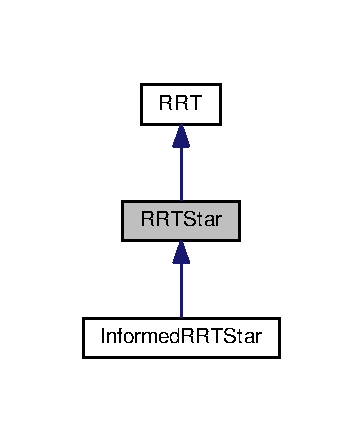
\includegraphics[width=174pt]{classRRTStar__inherit__graph}
\end{center}
\end{figure}


Collaboration diagram for R\+R\+T\+Star\+:
\nopagebreak
\begin{figure}[H]
\begin{center}
\leavevmode
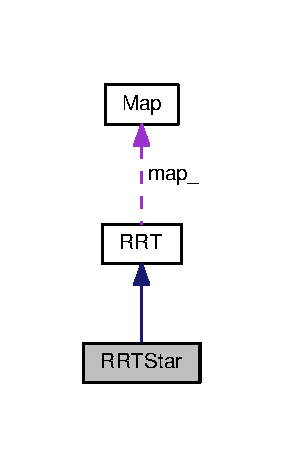
\includegraphics[width=136pt]{classRRTStar__coll__graph}
\end{center}
\end{figure}
\subsection*{Public Member Functions}
\begin{DoxyCompactItemize}
\item 
\hyperlink{classRRTStar_aa3305dbcb77c5c47166fdfbc14817802}{R\+R\+T\+Star} ()
\begin{DoxyCompactList}\small\item\em Default constructor for \hyperlink{classRRT}{R\+RT} Star. Prints basic information regarding planner. \end{DoxyCompactList}\item 
\hyperlink{classRRTStar_adbaa4004aaff73307684524b9a3a8c27}{$\sim$\+R\+R\+T\+Star} ()
\begin{DoxyCompactList}\small\item\em Destructor for \hyperlink{classRRT}{R\+RT} Star. \end{DoxyCompactList}\item 
std\+::pair$<$ size\+\_\+t, double $>$ \hyperlink{classRRTStar_ae2b78463af6072b4f7efa5188a530d54}{get\+Planner\+Params} ()
\begin{DoxyCompactList}\small\item\em function to return \hyperlink{classRRT}{R\+RT} star planner parameters \end{DoxyCompactList}\item 
void \hyperlink{classRRTStar_a1205f9b17419186be4a575151e68f304}{set\+Start\+And\+Goal} (const std\+::vector$<$ double $>$ \&start, const std\+::vector$<$ double $>$ \&goal)
\begin{DoxyCompactList}\small\item\em setter function to define the environment \end{DoxyCompactList}\item 
std\+::shared\+\_\+ptr$<$ \hyperlink{classRRTNode}{R\+R\+T\+Node} $>$ \hyperlink{classRRTStar_ac8825e6654bc43d7d82918451e09ea89}{find\+Closest\+Tree\+Node} (const std\+::vector$<$ double $>$ \&random\+Node)
\begin{DoxyCompactList}\small\item\em finds the closest node in the tree to a given randomly sampled node in the environment \end{DoxyCompactList}\item 
std\+::shared\+\_\+ptr$<$ \hyperlink{classRRTNode}{R\+R\+T\+Node} $>$ \hyperlink{classRRTStar_a6758b1eeb5b6d2f883d710a9bf8d2387}{rewire\+R\+R\+Tree} (const std\+::vector$<$ double $>$ \&new\+Node, std\+::shared\+\_\+ptr$<$ \hyperlink{classRRTNode}{R\+R\+T\+Node} $>$ \&current\+Parent)
\begin{DoxyCompactList}\small\item\em finds out if a better parent exists based on cummulative cost to come (cost to arrive a the node from start node) for a given node \end{DoxyCompactList}\item 
void \hyperlink{classRRTStar_a3b1f7e66c99881faa190034b0ff2b101}{append\+R\+R\+Tree} (const std\+::vector$<$ double $>$ \&valid\+Node, const std\+::shared\+\_\+ptr$<$ \hyperlink{classRRTNode}{R\+R\+T\+Node} $>$ \&valid\+Node\+Parent)
\begin{DoxyCompactList}\small\item\em appends the R\+R\+T\+Star\+Tree in the workspace with the new valid node \end{DoxyCompactList}\item 
std\+::vector$<$ std\+::pair$<$ double, double $>$ $>$ \hyperlink{classRRTStar_a9d415973b5fbafa4435203fb56ac3357}{get\+Planner\+Path} ()
\begin{DoxyCompactList}\small\item\em returns a path found by the \hyperlink{classRRT}{R\+RT} Star algorithm as a set of waypoints \end{DoxyCompactList}\item 
std\+::shared\+\_\+ptr$<$ \hyperlink{classRRTNode}{R\+R\+T\+Node} $>$ \hyperlink{classRRTStar_a859d863be7b83876119f89b8bc8c671e}{get\+Goal\+Node\+Ptr} ()
\begin{DoxyCompactList}\small\item\em returns a pointer to the object of goal node \end{DoxyCompactList}\item 
std\+::vector$<$ \hyperlink{classRRTNode}{R\+R\+T\+Node} $>$ \hyperlink{classRRTStar_ad63c0ccb78ae3bbd9c4e8b58f6299abe}{get\+R\+R\+T\+Star\+Tree} ()
\begin{DoxyCompactList}\small\item\em returns the tree resulting from the \hyperlink{classRRT}{R\+RT} Star algorithm \end{DoxyCompactList}\item 
virtual void \hyperlink{classRRTStar_a5018db145f3a5bb5b4a13b710009ae55}{run\+Planner} ()
\begin{DoxyCompactList}\small\item\em starts the execution of the \hyperlink{classRRT}{R\+RT} Star planning algorithm \end{DoxyCompactList}\item 
virtual void \hyperlink{classRRTStar_a713736e18edd589d262dd4c2efc1e18d}{reset\+Planner} ()
\begin{DoxyCompactList}\small\item\em resets the planner by clearing all member varibles of \hyperlink{classRRT}{R\+RT} Star class planner object \end{DoxyCompactList}\end{DoxyCompactItemize}
\subsection*{Public Attributes}
\begin{DoxyCompactItemize}
\item 
std\+::vector$<$ \hyperlink{classRRTNode}{R\+R\+T\+Node} $>$ \hyperlink{classRRTStar_a51cf408ef0d76ee5ee82726fc7bd26a5}{R\+R\+T\+Star\+Tree}
\begin{DoxyCompactList}\small\item\em Define the datastructure to hold the tree. \end{DoxyCompactList}\item 
size\+\_\+t \hyperlink{classRRTStar_a08084959938e25bff534134845d42e14}{max\+Iterations\+\_\+}
\item 
const double \hyperlink{classRRTStar_a9a7ceb082951fc07e20f6704fbb1c58e}{rewire\+Range\+\_\+}
\item 
std\+::vector$<$ std\+::shared\+\_\+ptr$<$ \hyperlink{classRRTNode}{R\+R\+T\+Node} $>$ $>$ \hyperlink{classRRTStar_a6a887af80bd8006376389011f27f7cba}{rewire\+Nodes\+\_\+}
\item 
std\+::shared\+\_\+ptr$<$ \hyperlink{classRRTNode}{R\+R\+T\+Node} $>$ \hyperlink{classRRTStar_a32f7b15e9ea09994a696310bca09bc19}{goal\+Node\+Ptr}
\end{DoxyCompactItemize}


\subsection{Detailed Description}
Class \hyperlink{classRRT}{R\+RT}, derived from class \hyperlink{classRRT}{R\+RT} The following class \hyperlink{classRRT}{R\+RT} Star optimizes the path found by \hyperlink{classRRT}{R\+RT} algorithm using cost to come to rewire the path and the tree nodes as well. 

\subsection{Constructor \& Destructor Documentation}
\index{R\+R\+T\+Star@{R\+R\+T\+Star}!R\+R\+T\+Star@{R\+R\+T\+Star}}
\index{R\+R\+T\+Star@{R\+R\+T\+Star}!R\+R\+T\+Star@{R\+R\+T\+Star}}
\subsubsection[{\texorpdfstring{R\+R\+T\+Star()}{RRTStar()}}]{\setlength{\rightskip}{0pt plus 5cm}R\+R\+T\+Star\+::\+R\+R\+T\+Star (
\begin{DoxyParamCaption}
{}
\end{DoxyParamCaption}
)}\hypertarget{classRRTStar_aa3305dbcb77c5c47166fdfbc14817802}{}\label{classRRTStar_aa3305dbcb77c5c47166fdfbc14817802}


Default constructor for \hyperlink{classRRT}{R\+RT} Star. Prints basic information regarding planner. 


\begin{DoxyParams}{Parameters}
{\em none} & \\
\hline
\end{DoxyParams}
\begin{DoxyReturn}{Returns}
void 
\end{DoxyReturn}
\index{R\+R\+T\+Star@{R\+R\+T\+Star}!````~R\+R\+T\+Star@{$\sim$\+R\+R\+T\+Star}}
\index{````~R\+R\+T\+Star@{$\sim$\+R\+R\+T\+Star}!R\+R\+T\+Star@{R\+R\+T\+Star}}
\subsubsection[{\texorpdfstring{$\sim$\+R\+R\+T\+Star()}{~RRTStar()}}]{\setlength{\rightskip}{0pt plus 5cm}R\+R\+T\+Star\+::$\sim$\+R\+R\+T\+Star (
\begin{DoxyParamCaption}
{}
\end{DoxyParamCaption}
)}\hypertarget{classRRTStar_adbaa4004aaff73307684524b9a3a8c27}{}\label{classRRTStar_adbaa4004aaff73307684524b9a3a8c27}


Destructor for \hyperlink{classRRT}{R\+RT} Star. 


\begin{DoxyParams}{Parameters}
{\em none} & \\
\hline
\end{DoxyParams}
\begin{DoxyReturn}{Returns}
void 
\end{DoxyReturn}


\subsection{Member Function Documentation}
\index{R\+R\+T\+Star@{R\+R\+T\+Star}!append\+R\+R\+Tree@{append\+R\+R\+Tree}}
\index{append\+R\+R\+Tree@{append\+R\+R\+Tree}!R\+R\+T\+Star@{R\+R\+T\+Star}}
\subsubsection[{\texorpdfstring{append\+R\+R\+Tree(const std\+::vector$<$ double $>$ \&valid\+Node, const std\+::shared\+\_\+ptr$<$ R\+R\+T\+Node $>$ \&valid\+Node\+Parent)}{appendRRTree(const std::vector< double > &validNode, const std::shared_ptr< RRTNode > &validNodeParent)}}]{\setlength{\rightskip}{0pt plus 5cm}void R\+R\+T\+Star\+::append\+R\+R\+Tree (
\begin{DoxyParamCaption}
\item[{const std\+::vector$<$ double $>$ \&}]{valid\+Node, }
\item[{const std\+::shared\+\_\+ptr$<$ {\bf R\+R\+T\+Node} $>$ \&}]{valid\+Node\+Parent}
\end{DoxyParamCaption}
)\hspace{0.3cm}{\ttfamily [virtual]}}\hypertarget{classRRTStar_a3b1f7e66c99881faa190034b0ff2b101}{}\label{classRRTStar_a3b1f7e66c99881faa190034b0ff2b101}


appends the R\+R\+T\+Star\+Tree in the workspace with the new valid node 


\begin{DoxyParams}{Parameters}
{\em valid\+Node} & is the newly generated node at a drivable distance to the current tree in the environment as a vector of double elements \mbox{[}x,y\mbox{]} valid\+Node\+Parent is the pointer to the object of class \hyperlink{classRRT}{R\+RT} pointing to the parent of the valid\+Node \\
\hline
\end{DoxyParams}
\begin{DoxyReturn}{Returns}
void 
\end{DoxyReturn}


Reimplemented from \hyperlink{classRRT_a2629b145454f54cca6a1ad796c27e900}{R\+RT}.

\index{R\+R\+T\+Star@{R\+R\+T\+Star}!find\+Closest\+Tree\+Node@{find\+Closest\+Tree\+Node}}
\index{find\+Closest\+Tree\+Node@{find\+Closest\+Tree\+Node}!R\+R\+T\+Star@{R\+R\+T\+Star}}
\subsubsection[{\texorpdfstring{find\+Closest\+Tree\+Node(const std\+::vector$<$ double $>$ \&random\+Node)}{findClosestTreeNode(const std::vector< double > &randomNode)}}]{\setlength{\rightskip}{0pt plus 5cm}std\+::shared\+\_\+ptr$<${\bf R\+R\+T\+Node}$>$ R\+R\+T\+Star\+::find\+Closest\+Tree\+Node (
\begin{DoxyParamCaption}
\item[{const std\+::vector$<$ double $>$ \&}]{random\+Node}
\end{DoxyParamCaption}
)\hspace{0.3cm}{\ttfamily [virtual]}}\hypertarget{classRRTStar_ac8825e6654bc43d7d82918451e09ea89}{}\label{classRRTStar_ac8825e6654bc43d7d82918451e09ea89}


finds the closest node in the tree to a given randomly sampled node in the environment 


\begin{DoxyParams}{Parameters}
{\em random\+Node} & is the randomly sampled node in the environment as a vector of double elements \\
\hline
\end{DoxyParams}
\begin{DoxyReturn}{Returns}
A smart pointer (shared\+\_\+ptr) pointing to the object of the closest tree node 
\end{DoxyReturn}


Reimplemented from \hyperlink{classRRT_ae581ca8e7858e75e3958596f9dd57390}{R\+RT}.

\index{R\+R\+T\+Star@{R\+R\+T\+Star}!get\+Goal\+Node\+Ptr@{get\+Goal\+Node\+Ptr}}
\index{get\+Goal\+Node\+Ptr@{get\+Goal\+Node\+Ptr}!R\+R\+T\+Star@{R\+R\+T\+Star}}
\subsubsection[{\texorpdfstring{get\+Goal\+Node\+Ptr()}{getGoalNodePtr()}}]{\setlength{\rightskip}{0pt plus 5cm}std\+::shared\+\_\+ptr$<${\bf R\+R\+T\+Node}$>$ R\+R\+T\+Star\+::get\+Goal\+Node\+Ptr (
\begin{DoxyParamCaption}
{}
\end{DoxyParamCaption}
)}\hypertarget{classRRTStar_a859d863be7b83876119f89b8bc8c671e}{}\label{classRRTStar_a859d863be7b83876119f89b8bc8c671e}


returns a pointer to the object of goal node 


\begin{DoxyParams}{Parameters}
{\em none} & \\
\hline
\end{DoxyParams}
\begin{DoxyReturn}{Returns}
a pointer pointing to the object of class \hyperlink{classRRTNode}{R\+R\+T\+Node} containing the goal node 
\end{DoxyReturn}
\index{R\+R\+T\+Star@{R\+R\+T\+Star}!get\+Planner\+Params@{get\+Planner\+Params}}
\index{get\+Planner\+Params@{get\+Planner\+Params}!R\+R\+T\+Star@{R\+R\+T\+Star}}
\subsubsection[{\texorpdfstring{get\+Planner\+Params()}{getPlannerParams()}}]{\setlength{\rightskip}{0pt plus 5cm}std\+::pair$<$size\+\_\+t, double$>$ R\+R\+T\+Star\+::get\+Planner\+Params (
\begin{DoxyParamCaption}
{}
\end{DoxyParamCaption}
)}\hypertarget{classRRTStar_ae2b78463af6072b4f7efa5188a530d54}{}\label{classRRTStar_ae2b78463af6072b4f7efa5188a530d54}


function to return \hyperlink{classRRT}{R\+RT} star planner parameters 


\begin{DoxyParams}{Parameters}
{\em none} & \\
\hline
\end{DoxyParams}
\begin{DoxyReturn}{Returns}
pair of values (unsigned int, double) defining the max iterations and drive paramater respectively 
\end{DoxyReturn}
\index{R\+R\+T\+Star@{R\+R\+T\+Star}!get\+Planner\+Path@{get\+Planner\+Path}}
\index{get\+Planner\+Path@{get\+Planner\+Path}!R\+R\+T\+Star@{R\+R\+T\+Star}}
\subsubsection[{\texorpdfstring{get\+Planner\+Path()}{getPlannerPath()}}]{\setlength{\rightskip}{0pt plus 5cm}std\+::vector$<$std\+::pair$<$double, double$>$ $>$ R\+R\+T\+Star\+::get\+Planner\+Path (
\begin{DoxyParamCaption}
{}
\end{DoxyParamCaption}
)\hspace{0.3cm}{\ttfamily [virtual]}}\hypertarget{classRRTStar_a9d415973b5fbafa4435203fb56ac3357}{}\label{classRRTStar_a9d415973b5fbafa4435203fb56ac3357}


returns a path found by the \hyperlink{classRRT}{R\+RT} Star algorithm as a set of waypoints 


\begin{DoxyParams}{Parameters}
{\em none} & \\
\hline
\end{DoxyParams}
\begin{DoxyReturn}{Returns}
vector of pair of double elements \mbox{[}x,y\mbox{]} representing the set of waypoints 
\end{DoxyReturn}


Reimplemented from \hyperlink{classRRT_a35e29366864cebacda5cd52c1febaa73}{R\+RT}.

\index{R\+R\+T\+Star@{R\+R\+T\+Star}!get\+R\+R\+T\+Star\+Tree@{get\+R\+R\+T\+Star\+Tree}}
\index{get\+R\+R\+T\+Star\+Tree@{get\+R\+R\+T\+Star\+Tree}!R\+R\+T\+Star@{R\+R\+T\+Star}}
\subsubsection[{\texorpdfstring{get\+R\+R\+T\+Star\+Tree()}{getRRTStarTree()}}]{\setlength{\rightskip}{0pt plus 5cm}std\+::vector$<${\bf R\+R\+T\+Node}$>$ R\+R\+T\+Star\+::get\+R\+R\+T\+Star\+Tree (
\begin{DoxyParamCaption}
{}
\end{DoxyParamCaption}
)}\hypertarget{classRRTStar_ad63c0ccb78ae3bbd9c4e8b58f6299abe}{}\label{classRRTStar_ad63c0ccb78ae3bbd9c4e8b58f6299abe}


returns the tree resulting from the \hyperlink{classRRT}{R\+RT} Star algorithm 


\begin{DoxyParams}{Parameters}
{\em none} & \\
\hline
\end{DoxyParams}
\begin{DoxyReturn}{Returns}
vector of nodes i.\+e objects of \hyperlink{classRRTNode}{R\+R\+T\+Node} class 
\end{DoxyReturn}
\index{R\+R\+T\+Star@{R\+R\+T\+Star}!reset\+Planner@{reset\+Planner}}
\index{reset\+Planner@{reset\+Planner}!R\+R\+T\+Star@{R\+R\+T\+Star}}
\subsubsection[{\texorpdfstring{reset\+Planner()}{resetPlanner()}}]{\setlength{\rightskip}{0pt plus 5cm}virtual void R\+R\+T\+Star\+::reset\+Planner (
\begin{DoxyParamCaption}
{}
\end{DoxyParamCaption}
)\hspace{0.3cm}{\ttfamily [virtual]}}\hypertarget{classRRTStar_a713736e18edd589d262dd4c2efc1e18d}{}\label{classRRTStar_a713736e18edd589d262dd4c2efc1e18d}


resets the planner by clearing all member varibles of \hyperlink{classRRT}{R\+RT} Star class planner object 


\begin{DoxyParams}{Parameters}
{\em none} & \\
\hline
\end{DoxyParams}
\begin{DoxyReturn}{Returns}
void 
\end{DoxyReturn}


Reimplemented from \hyperlink{classRRT_a952ef4be01547b013ce5c64d912fe680}{R\+RT}.



Reimplemented in \hyperlink{classInformedRRTStar_ac13574a2c2a765599ef42283b069a471}{Informed\+R\+R\+T\+Star}.

\index{R\+R\+T\+Star@{R\+R\+T\+Star}!rewire\+R\+R\+Tree@{rewire\+R\+R\+Tree}}
\index{rewire\+R\+R\+Tree@{rewire\+R\+R\+Tree}!R\+R\+T\+Star@{R\+R\+T\+Star}}
\subsubsection[{\texorpdfstring{rewire\+R\+R\+Tree(const std\+::vector$<$ double $>$ \&new\+Node, std\+::shared\+\_\+ptr$<$ R\+R\+T\+Node $>$ \&current\+Parent)}{rewireRRTree(const std::vector< double > &newNode, std::shared_ptr< RRTNode > &currentParent)}}]{\setlength{\rightskip}{0pt plus 5cm}std\+::shared\+\_\+ptr$<${\bf R\+R\+T\+Node}$>$ R\+R\+T\+Star\+::rewire\+R\+R\+Tree (
\begin{DoxyParamCaption}
\item[{const std\+::vector$<$ double $>$ \&}]{new\+Node, }
\item[{std\+::shared\+\_\+ptr$<$ {\bf R\+R\+T\+Node} $>$ \&}]{current\+Parent}
\end{DoxyParamCaption}
)}\hypertarget{classRRTStar_a6758b1eeb5b6d2f883d710a9bf8d2387}{}\label{classRRTStar_a6758b1eeb5b6d2f883d710a9bf8d2387}


finds out if a better parent exists based on cummulative cost to come (cost to arrive a the node from start node) for a given node 


\begin{DoxyParams}{Parameters}
{\em new\+Node} & is the latest node added to the tree as a vector of double elements current\+Parent is the pointer to parent object of new\+Node \\
\hline
\end{DoxyParams}
\begin{DoxyReturn}{Returns}
A smart pointer (shared\+\_\+ptr) pointing to the object of the parent node which minimizes the cost to come for the new\+Node 
\end{DoxyReturn}
\index{R\+R\+T\+Star@{R\+R\+T\+Star}!run\+Planner@{run\+Planner}}
\index{run\+Planner@{run\+Planner}!R\+R\+T\+Star@{R\+R\+T\+Star}}
\subsubsection[{\texorpdfstring{run\+Planner()}{runPlanner()}}]{\setlength{\rightskip}{0pt plus 5cm}virtual void R\+R\+T\+Star\+::run\+Planner (
\begin{DoxyParamCaption}
{}
\end{DoxyParamCaption}
)\hspace{0.3cm}{\ttfamily [virtual]}}\hypertarget{classRRTStar_a5018db145f3a5bb5b4a13b710009ae55}{}\label{classRRTStar_a5018db145f3a5bb5b4a13b710009ae55}


starts the execution of the \hyperlink{classRRT}{R\+RT} Star planning algorithm 


\begin{DoxyParams}{Parameters}
{\em none} & \\
\hline
\end{DoxyParams}
\begin{DoxyReturn}{Returns}
void 
\end{DoxyReturn}


Reimplemented from \hyperlink{classRRT_a57a214360eb86fc63d7300bc1ea94fde}{R\+RT}.



Reimplemented in \hyperlink{classInformedRRTStar_afbd7ccc52e9d6dfe734ffcb1bc386234}{Informed\+R\+R\+T\+Star}.

\index{R\+R\+T\+Star@{R\+R\+T\+Star}!set\+Start\+And\+Goal@{set\+Start\+And\+Goal}}
\index{set\+Start\+And\+Goal@{set\+Start\+And\+Goal}!R\+R\+T\+Star@{R\+R\+T\+Star}}
\subsubsection[{\texorpdfstring{set\+Start\+And\+Goal(const std\+::vector$<$ double $>$ \&start, const std\+::vector$<$ double $>$ \&goal)}{setStartAndGoal(const std::vector< double > &start, const std::vector< double > &goal)}}]{\setlength{\rightskip}{0pt plus 5cm}void R\+R\+T\+Star\+::set\+Start\+And\+Goal (
\begin{DoxyParamCaption}
\item[{const std\+::vector$<$ double $>$ \&}]{start, }
\item[{const std\+::vector$<$ double $>$ \&}]{goal}
\end{DoxyParamCaption}
)\hspace{0.3cm}{\ttfamily [virtual]}}\hypertarget{classRRTStar_a1205f9b17419186be4a575151e68f304}{}\label{classRRTStar_a1205f9b17419186be4a575151e68f304}


setter function to define the environment 


\begin{DoxyParams}{Parameters}
{\em boundary} & is a vector of paired points \mbox{[}x,y\mbox{]} defining the boundary vertices. obstacles is a vector of obstacle container which in turn is a vector of double points \mbox{[}x1,y1,x2,y2...xN,yN\mbox{]} defining the boundary vertices of an obstacle in the environment. \\
\hline
\end{DoxyParams}
\begin{DoxyReturn}{Returns}
void 
\end{DoxyReturn}


Reimplemented from \hyperlink{classRRT_a4954f750e5aedfea24fb52771bd5b1af}{R\+RT}.



\subsection{Member Data Documentation}
\index{R\+R\+T\+Star@{R\+R\+T\+Star}!goal\+Node\+Ptr@{goal\+Node\+Ptr}}
\index{goal\+Node\+Ptr@{goal\+Node\+Ptr}!R\+R\+T\+Star@{R\+R\+T\+Star}}
\subsubsection[{\texorpdfstring{goal\+Node\+Ptr}{goalNodePtr}}]{\setlength{\rightskip}{0pt plus 5cm}std\+::shared\+\_\+ptr$<${\bf R\+R\+T\+Node}$>$ R\+R\+T\+Star\+::goal\+Node\+Ptr}\hypertarget{classRRTStar_a32f7b15e9ea09994a696310bca09bc19}{}\label{classRRTStar_a32f7b15e9ea09994a696310bca09bc19}
Pointer to the object of class \hyperlink{classRRTNode}{R\+R\+T\+Node} denoting the goal node \index{R\+R\+T\+Star@{R\+R\+T\+Star}!max\+Iterations\+\_\+@{max\+Iterations\+\_\+}}
\index{max\+Iterations\+\_\+@{max\+Iterations\+\_\+}!R\+R\+T\+Star@{R\+R\+T\+Star}}
\subsubsection[{\texorpdfstring{max\+Iterations\+\_\+}{maxIterations_}}]{\setlength{\rightskip}{0pt plus 5cm}size\+\_\+t R\+R\+T\+Star\+::max\+Iterations\+\_\+}\hypertarget{classRRTStar_a08084959938e25bff534134845d42e14}{}\label{classRRTStar_a08084959938e25bff534134845d42e14}
{\bfseries Initial value\+:}
\begin{DoxyCode}
=
      plannerParams\_.first
\end{DoxyCode}
Max iterations the algorithm runs for. Same as parent class \hyperlink{classRRT}{R\+RT}. \index{R\+R\+T\+Star@{R\+R\+T\+Star}!rewire\+Nodes\+\_\+@{rewire\+Nodes\+\_\+}}
\index{rewire\+Nodes\+\_\+@{rewire\+Nodes\+\_\+}!R\+R\+T\+Star@{R\+R\+T\+Star}}
\subsubsection[{\texorpdfstring{rewire\+Nodes\+\_\+}{rewireNodes_}}]{\setlength{\rightskip}{0pt plus 5cm}std\+::vector$<$std\+::shared\+\_\+ptr$<${\bf R\+R\+T\+Node}$>$ $>$ R\+R\+T\+Star\+::rewire\+Nodes\+\_\+}\hypertarget{classRRTStar_a6a887af80bd8006376389011f27f7cba}{}\label{classRRTStar_a6a887af80bd8006376389011f27f7cba}
Vector to hold possible rewirable nodes for a given node \index{R\+R\+T\+Star@{R\+R\+T\+Star}!rewire\+Range\+\_\+@{rewire\+Range\+\_\+}}
\index{rewire\+Range\+\_\+@{rewire\+Range\+\_\+}!R\+R\+T\+Star@{R\+R\+T\+Star}}
\subsubsection[{\texorpdfstring{rewire\+Range\+\_\+}{rewireRange_}}]{\setlength{\rightskip}{0pt plus 5cm}const double R\+R\+T\+Star\+::rewire\+Range\+\_\+}\hypertarget{classRRTStar_a9a7ceb082951fc07e20f6704fbb1c58e}{}\label{classRRTStar_a9a7ceb082951fc07e20f6704fbb1c58e}
{\bfseries Initial value\+:}
\begin{DoxyCode}
=
      2.0 * plannerParams\_.second
\end{DoxyCode}
Range around a node to check for possible new parent to rewire to \index{R\+R\+T\+Star@{R\+R\+T\+Star}!R\+R\+T\+Star\+Tree@{R\+R\+T\+Star\+Tree}}
\index{R\+R\+T\+Star\+Tree@{R\+R\+T\+Star\+Tree}!R\+R\+T\+Star@{R\+R\+T\+Star}}
\subsubsection[{\texorpdfstring{R\+R\+T\+Star\+Tree}{RRTStarTree}}]{\setlength{\rightskip}{0pt plus 5cm}std\+::vector$<${\bf R\+R\+T\+Node}$>$ R\+R\+T\+Star\+::\+R\+R\+T\+Star\+Tree}\hypertarget{classRRTStar_a51cf408ef0d76ee5ee82726fc7bd26a5}{}\label{classRRTStar_a51cf408ef0d76ee5ee82726fc7bd26a5}
{\bfseries Initial value\+:}
\begin{DoxyCode}
=
      \hyperlink{classRRT_aba9e08111e7b76cd72acf2d0d4d560ae}{getRRTree}()
\end{DoxyCode}


Define the datastructure to hold the tree. 



The documentation for this class was generated from the following file\+:\begin{DoxyCompactItemize}
\item 
/home/srinidhi/\+Git\+Hub/\+My Repos/\+E\+N\+P\+M808\+X-\/\+Midterm-\/\+Informed\+R\+R\+T\+Star/include/\hyperlink{RRTStar_8hpp}{R\+R\+T\+Star.\+hpp}\end{DoxyCompactItemize}

\hypertarget{structmatplotlibcpp_1_1select__npy__type}{}\section{matplotlibcpp\+:\+:select\+\_\+npy\+\_\+type$<$ T $>$ Struct Template Reference}
\label{structmatplotlibcpp_1_1select__npy__type}\index{matplotlibcpp\+::select\+\_\+npy\+\_\+type$<$ T $>$@{matplotlibcpp\+::select\+\_\+npy\+\_\+type$<$ T $>$}}
\subsection*{Static Public Attributes}
\begin{DoxyCompactItemize}
\item 
static const N\+P\+Y\+\_\+\+T\+Y\+P\+ES {\bfseries type} = N\+P\+Y\+\_\+\+N\+O\+T\+Y\+PE\hypertarget{structmatplotlibcpp_1_1select__npy__type_acbffa4e6e1d047b52e12330446816c9c}{}\label{structmatplotlibcpp_1_1select__npy__type_acbffa4e6e1d047b52e12330446816c9c}

\end{DoxyCompactItemize}


The documentation for this struct was generated from the following file\+:\begin{DoxyCompactItemize}
\item 
/home/srinidhi/\+Git\+Hub/\+My Repos/\+E\+N\+P\+M808\+X-\/\+Midterm-\/\+Informed\+R\+R\+T\+Star/include/matplotlibcpp.\+h\end{DoxyCompactItemize}

\hypertarget{structmatplotlibcpp_1_1select__npy__type_3_01bool_01_4}{}\section{matplotlibcpp\+:\+:select\+\_\+npy\+\_\+type$<$ bool $>$ Struct Template Reference}
\label{structmatplotlibcpp_1_1select__npy__type_3_01bool_01_4}\index{matplotlibcpp\+::select\+\_\+npy\+\_\+type$<$ bool $>$@{matplotlibcpp\+::select\+\_\+npy\+\_\+type$<$ bool $>$}}
\subsection*{Static Public Attributes}
\begin{DoxyCompactItemize}
\item 
static const N\+P\+Y\+\_\+\+T\+Y\+P\+ES {\bfseries type} = N\+P\+Y\+\_\+\+B\+O\+OL\hypertarget{structmatplotlibcpp_1_1select__npy__type_3_01bool_01_4_a79dc3db61a3b0f4796a29d067d5dd374}{}\label{structmatplotlibcpp_1_1select__npy__type_3_01bool_01_4_a79dc3db61a3b0f4796a29d067d5dd374}

\end{DoxyCompactItemize}


The documentation for this struct was generated from the following file\+:\begin{DoxyCompactItemize}
\item 
/home/srinidhi/\+Git\+Hub/\+My Repos/\+E\+N\+P\+M808\+X-\/\+Midterm-\/\+Informed\+R\+R\+T\+Star/include/matplotlibcpp.\+h\end{DoxyCompactItemize}

\hypertarget{structmatplotlibcpp_1_1select__npy__type_3_01double_01_4}{}\section{matplotlibcpp\+:\+:select\+\_\+npy\+\_\+type$<$ double $>$ Struct Template Reference}
\label{structmatplotlibcpp_1_1select__npy__type_3_01double_01_4}\index{matplotlibcpp\+::select\+\_\+npy\+\_\+type$<$ double $>$@{matplotlibcpp\+::select\+\_\+npy\+\_\+type$<$ double $>$}}
\subsection*{Static Public Attributes}
\begin{DoxyCompactItemize}
\item 
static const N\+P\+Y\+\_\+\+T\+Y\+P\+ES {\bfseries type} = N\+P\+Y\+\_\+\+D\+O\+U\+B\+LE\hypertarget{structmatplotlibcpp_1_1select__npy__type_3_01double_01_4_a939edaf81fedb879c8c90ad13c98a709}{}\label{structmatplotlibcpp_1_1select__npy__type_3_01double_01_4_a939edaf81fedb879c8c90ad13c98a709}

\end{DoxyCompactItemize}


The documentation for this struct was generated from the following file\+:\begin{DoxyCompactItemize}
\item 
/home/srinidhi/\+Git\+Hub/\+My Repos/\+E\+N\+P\+M808\+X-\/\+Midterm-\/\+Informed\+R\+R\+T\+Star/include/matplotlibcpp.\+h\end{DoxyCompactItemize}

\hypertarget{structmatplotlibcpp_1_1select__npy__type_3_01float_01_4}{}\section{matplotlibcpp\+:\+:select\+\_\+npy\+\_\+type$<$ float $>$ Struct Template Reference}
\label{structmatplotlibcpp_1_1select__npy__type_3_01float_01_4}\index{matplotlibcpp\+::select\+\_\+npy\+\_\+type$<$ float $>$@{matplotlibcpp\+::select\+\_\+npy\+\_\+type$<$ float $>$}}
\subsection*{Static Public Attributes}
\begin{DoxyCompactItemize}
\item 
static const N\+P\+Y\+\_\+\+T\+Y\+P\+ES {\bfseries type} = N\+P\+Y\+\_\+\+F\+L\+O\+AT\hypertarget{structmatplotlibcpp_1_1select__npy__type_3_01float_01_4_a7bca025a3f0cb143e566e0f575bf7f6b}{}\label{structmatplotlibcpp_1_1select__npy__type_3_01float_01_4_a7bca025a3f0cb143e566e0f575bf7f6b}

\end{DoxyCompactItemize}


The documentation for this struct was generated from the following file\+:\begin{DoxyCompactItemize}
\item 
/home/srinidhi/\+Git\+Hub/\+My Repos/\+E\+N\+P\+M808\+X-\/\+Midterm-\/\+Informed\+R\+R\+T\+Star/include/matplotlibcpp.\+h\end{DoxyCompactItemize}

\hypertarget{structmatplotlibcpp_1_1select__npy__type_3_01int16__t_01_4}{}\section{matplotlibcpp\+:\+:select\+\_\+npy\+\_\+type$<$ int16\+\_\+t $>$ Struct Template Reference}
\label{structmatplotlibcpp_1_1select__npy__type_3_01int16__t_01_4}\index{matplotlibcpp\+::select\+\_\+npy\+\_\+type$<$ int16\+\_\+t $>$@{matplotlibcpp\+::select\+\_\+npy\+\_\+type$<$ int16\+\_\+t $>$}}
\subsection*{Static Public Attributes}
\begin{DoxyCompactItemize}
\item 
static const N\+P\+Y\+\_\+\+T\+Y\+P\+ES {\bfseries type} = N\+P\+Y\+\_\+\+S\+H\+O\+RT\hypertarget{structmatplotlibcpp_1_1select__npy__type_3_01int16__t_01_4_aa7e1803c594ccc58c2cd4c8818d5a158}{}\label{structmatplotlibcpp_1_1select__npy__type_3_01int16__t_01_4_aa7e1803c594ccc58c2cd4c8818d5a158}

\end{DoxyCompactItemize}


The documentation for this struct was generated from the following file\+:\begin{DoxyCompactItemize}
\item 
/home/srinidhi/\+Git\+Hub/\+My Repos/\+E\+N\+P\+M808\+X-\/\+Midterm-\/\+Informed\+R\+R\+T\+Star/include/matplotlibcpp.\+h\end{DoxyCompactItemize}

\hypertarget{structmatplotlibcpp_1_1select__npy__type_3_01int32__t_01_4}{}\section{matplotlibcpp\+:\+:select\+\_\+npy\+\_\+type$<$ int32\+\_\+t $>$ Struct Template Reference}
\label{structmatplotlibcpp_1_1select__npy__type_3_01int32__t_01_4}\index{matplotlibcpp\+::select\+\_\+npy\+\_\+type$<$ int32\+\_\+t $>$@{matplotlibcpp\+::select\+\_\+npy\+\_\+type$<$ int32\+\_\+t $>$}}
\subsection*{Static Public Attributes}
\begin{DoxyCompactItemize}
\item 
static const N\+P\+Y\+\_\+\+T\+Y\+P\+ES {\bfseries type} = N\+P\+Y\+\_\+\+I\+NT\hypertarget{structmatplotlibcpp_1_1select__npy__type_3_01int32__t_01_4_abcfd0c3dc5d5e92575c04747315cb4d5}{}\label{structmatplotlibcpp_1_1select__npy__type_3_01int32__t_01_4_abcfd0c3dc5d5e92575c04747315cb4d5}

\end{DoxyCompactItemize}


The documentation for this struct was generated from the following file\+:\begin{DoxyCompactItemize}
\item 
/home/srinidhi/\+Git\+Hub/\+My Repos/\+E\+N\+P\+M808\+X-\/\+Midterm-\/\+Informed\+R\+R\+T\+Star/include/matplotlibcpp.\+h\end{DoxyCompactItemize}

\hypertarget{structmatplotlibcpp_1_1select__npy__type_3_01int64__t_01_4}{}\section{matplotlibcpp\+:\+:select\+\_\+npy\+\_\+type$<$ int64\+\_\+t $>$ Struct Template Reference}
\label{structmatplotlibcpp_1_1select__npy__type_3_01int64__t_01_4}\index{matplotlibcpp\+::select\+\_\+npy\+\_\+type$<$ int64\+\_\+t $>$@{matplotlibcpp\+::select\+\_\+npy\+\_\+type$<$ int64\+\_\+t $>$}}
\subsection*{Static Public Attributes}
\begin{DoxyCompactItemize}
\item 
static const N\+P\+Y\+\_\+\+T\+Y\+P\+ES {\bfseries type} = N\+P\+Y\+\_\+\+I\+N\+T64\hypertarget{structmatplotlibcpp_1_1select__npy__type_3_01int64__t_01_4_a0d20ea35e520ad9381aca3c173f3f02d}{}\label{structmatplotlibcpp_1_1select__npy__type_3_01int64__t_01_4_a0d20ea35e520ad9381aca3c173f3f02d}

\end{DoxyCompactItemize}


The documentation for this struct was generated from the following file\+:\begin{DoxyCompactItemize}
\item 
/home/srinidhi/\+Git\+Hub/\+My Repos/\+E\+N\+P\+M808\+X-\/\+Midterm-\/\+Informed\+R\+R\+T\+Star/include/matplotlibcpp.\+h\end{DoxyCompactItemize}

\hypertarget{structmatplotlibcpp_1_1select__npy__type_3_01int8__t_01_4}{}\section{matplotlibcpp\+:\+:select\+\_\+npy\+\_\+type$<$ int8\+\_\+t $>$ Struct Template Reference}
\label{structmatplotlibcpp_1_1select__npy__type_3_01int8__t_01_4}\index{matplotlibcpp\+::select\+\_\+npy\+\_\+type$<$ int8\+\_\+t $>$@{matplotlibcpp\+::select\+\_\+npy\+\_\+type$<$ int8\+\_\+t $>$}}
\subsection*{Static Public Attributes}
\begin{DoxyCompactItemize}
\item 
static const N\+P\+Y\+\_\+\+T\+Y\+P\+ES {\bfseries type} = N\+P\+Y\+\_\+\+I\+N\+T8\hypertarget{structmatplotlibcpp_1_1select__npy__type_3_01int8__t_01_4_a74836a19458ed32ca8948a4337364eae}{}\label{structmatplotlibcpp_1_1select__npy__type_3_01int8__t_01_4_a74836a19458ed32ca8948a4337364eae}

\end{DoxyCompactItemize}


The documentation for this struct was generated from the following file\+:\begin{DoxyCompactItemize}
\item 
/home/srinidhi/\+Git\+Hub/\+My Repos/\+E\+N\+P\+M808\+X-\/\+Midterm-\/\+Informed\+R\+R\+T\+Star/include/matplotlibcpp.\+h\end{DoxyCompactItemize}

\hypertarget{structmatplotlibcpp_1_1select__npy__type_3_01uint16__t_01_4}{}\section{matplotlibcpp\+:\+:select\+\_\+npy\+\_\+type$<$ uint16\+\_\+t $>$ Struct Template Reference}
\label{structmatplotlibcpp_1_1select__npy__type_3_01uint16__t_01_4}\index{matplotlibcpp\+::select\+\_\+npy\+\_\+type$<$ uint16\+\_\+t $>$@{matplotlibcpp\+::select\+\_\+npy\+\_\+type$<$ uint16\+\_\+t $>$}}
\subsection*{Static Public Attributes}
\begin{DoxyCompactItemize}
\item 
static const N\+P\+Y\+\_\+\+T\+Y\+P\+ES {\bfseries type} = N\+P\+Y\+\_\+\+U\+S\+H\+O\+RT\hypertarget{structmatplotlibcpp_1_1select__npy__type_3_01uint16__t_01_4_aca209b33cc0bcaad16c01bff097a075f}{}\label{structmatplotlibcpp_1_1select__npy__type_3_01uint16__t_01_4_aca209b33cc0bcaad16c01bff097a075f}

\end{DoxyCompactItemize}


The documentation for this struct was generated from the following file\+:\begin{DoxyCompactItemize}
\item 
/home/srinidhi/\+Git\+Hub/\+My Repos/\+E\+N\+P\+M808\+X-\/\+Midterm-\/\+Informed\+R\+R\+T\+Star/include/matplotlibcpp.\+h\end{DoxyCompactItemize}

\hypertarget{structmatplotlibcpp_1_1select__npy__type_3_01uint32__t_01_4}{}\section{matplotlibcpp\+:\+:select\+\_\+npy\+\_\+type$<$ uint32\+\_\+t $>$ Struct Template Reference}
\label{structmatplotlibcpp_1_1select__npy__type_3_01uint32__t_01_4}\index{matplotlibcpp\+::select\+\_\+npy\+\_\+type$<$ uint32\+\_\+t $>$@{matplotlibcpp\+::select\+\_\+npy\+\_\+type$<$ uint32\+\_\+t $>$}}
\subsection*{Static Public Attributes}
\begin{DoxyCompactItemize}
\item 
static const N\+P\+Y\+\_\+\+T\+Y\+P\+ES {\bfseries type} = N\+P\+Y\+\_\+\+U\+L\+O\+NG\hypertarget{structmatplotlibcpp_1_1select__npy__type_3_01uint32__t_01_4_a21b0fbd17b661ef512cc1c3c728dfa60}{}\label{structmatplotlibcpp_1_1select__npy__type_3_01uint32__t_01_4_a21b0fbd17b661ef512cc1c3c728dfa60}

\end{DoxyCompactItemize}


The documentation for this struct was generated from the following file\+:\begin{DoxyCompactItemize}
\item 
/home/srinidhi/\+Git\+Hub/\+My Repos/\+E\+N\+P\+M808\+X-\/\+Midterm-\/\+Informed\+R\+R\+T\+Star/include/matplotlibcpp.\+h\end{DoxyCompactItemize}

\hypertarget{structmatplotlibcpp_1_1select__npy__type_3_01uint64__t_01_4}{}\section{matplotlibcpp\+:\+:select\+\_\+npy\+\_\+type$<$ uint64\+\_\+t $>$ Struct Template Reference}
\label{structmatplotlibcpp_1_1select__npy__type_3_01uint64__t_01_4}\index{matplotlibcpp\+::select\+\_\+npy\+\_\+type$<$ uint64\+\_\+t $>$@{matplotlibcpp\+::select\+\_\+npy\+\_\+type$<$ uint64\+\_\+t $>$}}
\subsection*{Static Public Attributes}
\begin{DoxyCompactItemize}
\item 
static const N\+P\+Y\+\_\+\+T\+Y\+P\+ES {\bfseries type} = N\+P\+Y\+\_\+\+U\+I\+N\+T64\hypertarget{structmatplotlibcpp_1_1select__npy__type_3_01uint64__t_01_4_a8d5871452f90ff04452f0416bee54fca}{}\label{structmatplotlibcpp_1_1select__npy__type_3_01uint64__t_01_4_a8d5871452f90ff04452f0416bee54fca}

\end{DoxyCompactItemize}


The documentation for this struct was generated from the following file\+:\begin{DoxyCompactItemize}
\item 
/home/srinidhi/\+Git\+Hub/\+My Repos/\+E\+N\+P\+M808\+X-\/\+Midterm-\/\+Informed\+R\+R\+T\+Star/include/matplotlibcpp.\+h\end{DoxyCompactItemize}

\hypertarget{structmatplotlibcpp_1_1select__npy__type_3_01uint8__t_01_4}{}\section{matplotlibcpp\+:\+:select\+\_\+npy\+\_\+type$<$ uint8\+\_\+t $>$ Struct Template Reference}
\label{structmatplotlibcpp_1_1select__npy__type_3_01uint8__t_01_4}\index{matplotlibcpp\+::select\+\_\+npy\+\_\+type$<$ uint8\+\_\+t $>$@{matplotlibcpp\+::select\+\_\+npy\+\_\+type$<$ uint8\+\_\+t $>$}}
\subsection*{Static Public Attributes}
\begin{DoxyCompactItemize}
\item 
static const N\+P\+Y\+\_\+\+T\+Y\+P\+ES {\bfseries type} = N\+P\+Y\+\_\+\+U\+I\+N\+T8\hypertarget{structmatplotlibcpp_1_1select__npy__type_3_01uint8__t_01_4_a6e80bfd252a69f14ff869c8b4fbb9e54}{}\label{structmatplotlibcpp_1_1select__npy__type_3_01uint8__t_01_4_a6e80bfd252a69f14ff869c8b4fbb9e54}

\end{DoxyCompactItemize}


The documentation for this struct was generated from the following file\+:\begin{DoxyCompactItemize}
\item 
/home/srinidhi/\+Git\+Hub/\+My Repos/\+E\+N\+P\+M808\+X-\/\+Midterm-\/\+Informed\+R\+R\+T\+Star/include/matplotlibcpp.\+h\end{DoxyCompactItemize}

\chapter{File Documentation}
\hypertarget{map_8hpp}{}\section{/home/srinidhi/\+Git\+Hub/\+My Repos/\+E\+N\+P\+M808\+X-\/\+Midterm-\/\+Informed\+R\+R\+T\+Star/include/map.hpp File Reference}
\label{map_8hpp}\index{/home/srinidhi/\+Git\+Hub/\+My Repos/\+E\+N\+P\+M808\+X-\/\+Midterm-\/\+Informed\+R\+R\+T\+Star/include/map.\+hpp@{/home/srinidhi/\+Git\+Hub/\+My Repos/\+E\+N\+P\+M808\+X-\/\+Midterm-\/\+Informed\+R\+R\+T\+Star/include/map.\+hpp}}


\hyperlink{classMap}{Map} class declaration.  


{\ttfamily \#include $<$utility$>$}\\*
{\ttfamily \#include $<$vector$>$}\\*
Include dependency graph for map.\+hpp\+:
\nopagebreak
\begin{figure}[H]
\begin{center}
\leavevmode
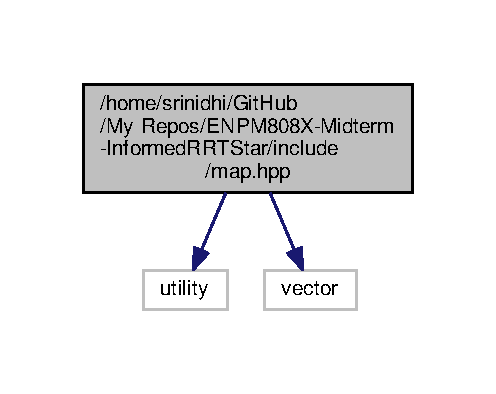
\includegraphics[width=238pt]{map_8hpp__incl}
\end{center}
\end{figure}
This graph shows which files directly or indirectly include this file\+:
\nopagebreak
\begin{figure}[H]
\begin{center}
\leavevmode
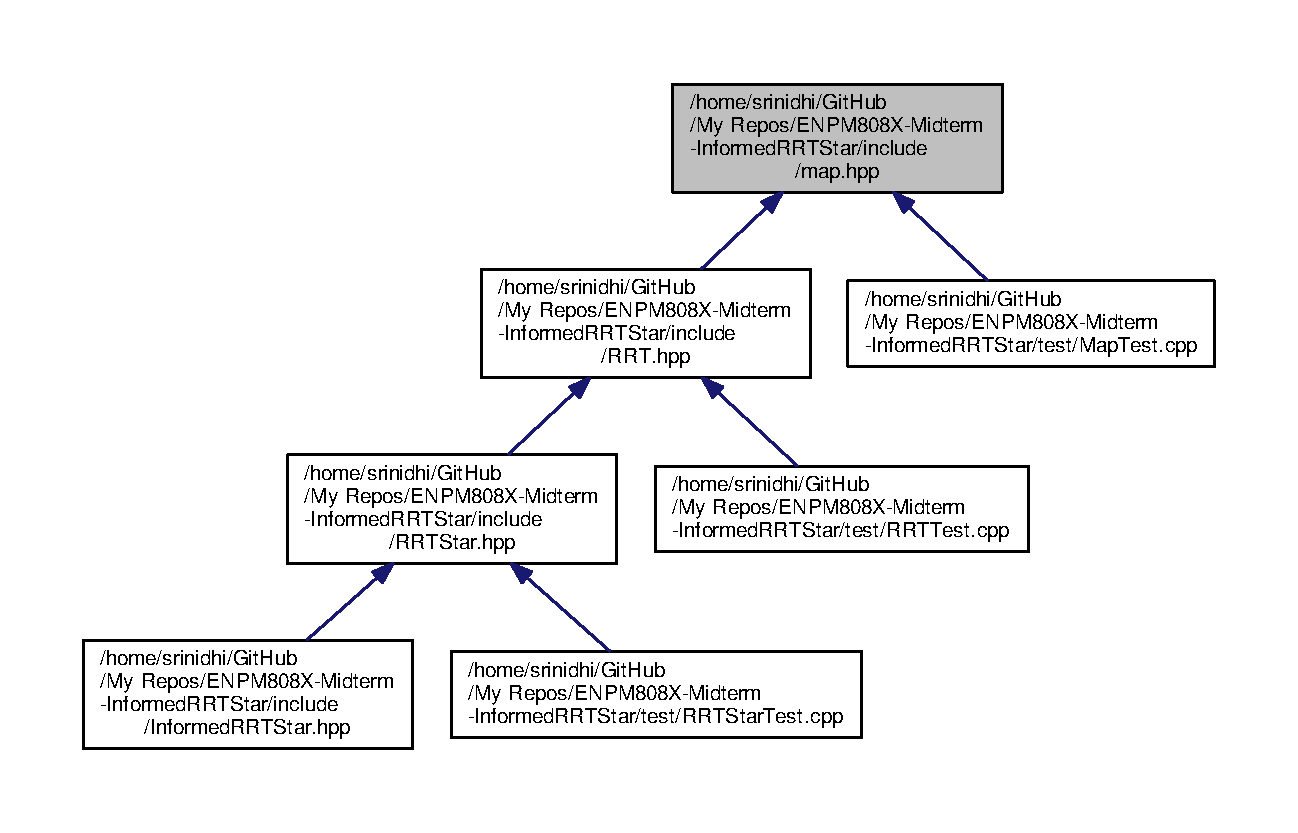
\includegraphics[width=350pt]{map_8hpp__dep__incl}
\end{center}
\end{figure}
\subsection*{Classes}
\begin{DoxyCompactItemize}
\item 
class \hyperlink{classMap}{Map}
\begin{DoxyCompactList}\small\item\em Class \hyperlink{classMap}{Map} The following class \hyperlink{classMap}{Map} aids in storing the layout of the environment. \end{DoxyCompactList}\end{DoxyCompactItemize}


\subsection{Detailed Description}
\hyperlink{classMap}{Map} class declaration. 

\begin{DoxyAuthor}{Author}
Srinidhi Sreenath (Srinidhi\+Sreenath) 
\end{DoxyAuthor}
\begin{DoxyDate}{Date}
10/7/2018 
\end{DoxyDate}
\begin{DoxyVersion}{Version}
1.\+0
\end{DoxyVersion}
\hypertarget{RRTTest_8cpp_DESCRIPTION}{}\subsection{D\+E\+S\+C\+R\+I\+P\+T\+I\+ON}\label{RRTTest_8cpp_DESCRIPTION}
Header file for class \hyperlink{classMap}{Map}. 
\hypertarget{RRT_8hpp}{}\section{/home/srinidhi/\+Git\+Hub/\+My Repos/\+E\+N\+P\+M808\+X-\/\+Midterm-\/\+Informed\+R\+R\+T\+Star/include/\+R\+RT.hpp File Reference}
\label{RRT_8hpp}\index{/home/srinidhi/\+Git\+Hub/\+My Repos/\+E\+N\+P\+M808\+X-\/\+Midterm-\/\+Informed\+R\+R\+T\+Star/include/\+R\+R\+T.\+hpp@{/home/srinidhi/\+Git\+Hub/\+My Repos/\+E\+N\+P\+M808\+X-\/\+Midterm-\/\+Informed\+R\+R\+T\+Star/include/\+R\+R\+T.\+hpp}}


\hyperlink{classRRT}{R\+RT} class declaration.  


{\ttfamily \#include \char`\"{}R\+R\+T\+Node.\+hpp\char`\"{}}\\*
{\ttfamily \#include \char`\"{}map.\+hpp\char`\"{}}\\*
Include dependency graph for R\+R\+T.\+hpp\+:
\nopagebreak
\begin{figure}[H]
\begin{center}
\leavevmode
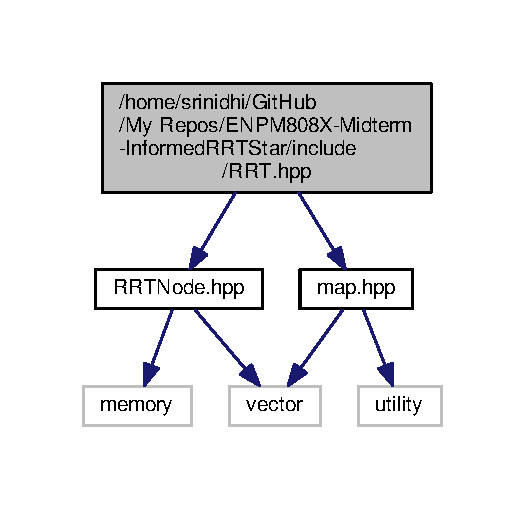
\includegraphics[width=252pt]{RRT_8hpp__incl}
\end{center}
\end{figure}
This graph shows which files directly or indirectly include this file\+:
\nopagebreak
\begin{figure}[H]
\begin{center}
\leavevmode
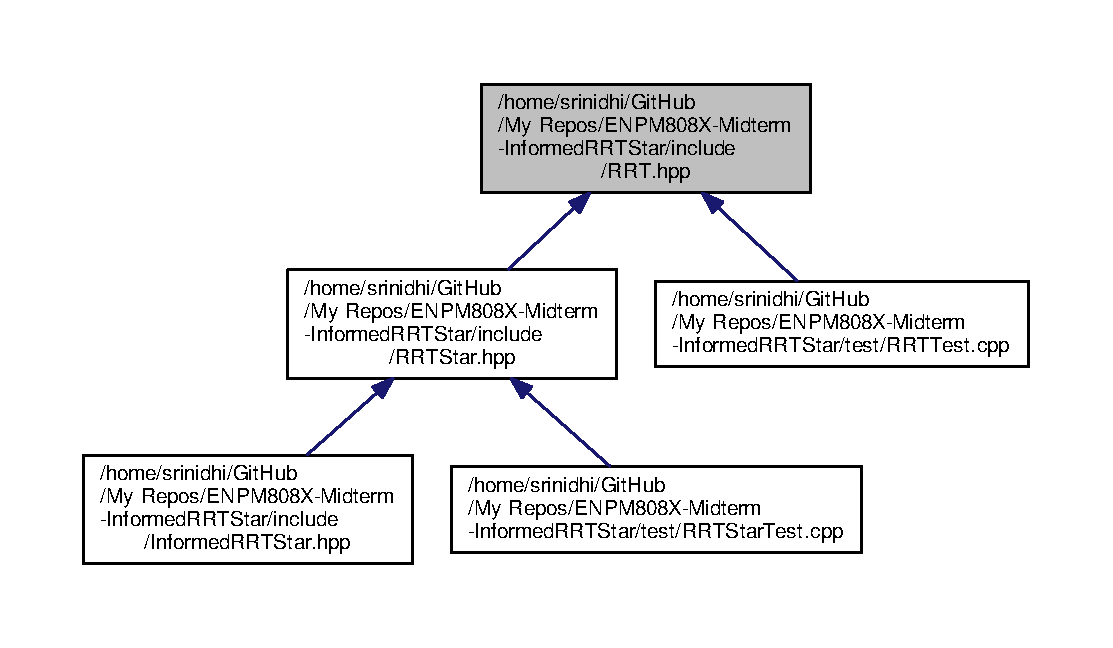
\includegraphics[width=350pt]{RRT_8hpp__dep__incl}
\end{center}
\end{figure}
\subsection*{Classes}
\begin{DoxyCompactItemize}
\item 
class \hyperlink{classRRT}{R\+RT}
\begin{DoxyCompactList}\small\item\em Class \hyperlink{classRRT}{R\+RT} The following class \hyperlink{classRRT}{R\+RT} implements the Rapidly-\/exploring random tree to find a path from start to goal in an environment. \end{DoxyCompactList}\end{DoxyCompactItemize}


\subsection{Detailed Description}
\hyperlink{classRRT}{R\+RT} class declaration. 

\begin{DoxyAuthor}{Author}
Srinidhi Sreenath (Srinidhi\+Sreenath) 
\end{DoxyAuthor}
\begin{DoxyDate}{Date}
10/11/2018 
\end{DoxyDate}
\begin{DoxyVersion}{Version}
1.\+0
\end{DoxyVersion}
\hypertarget{RRTTest_8cpp_DESCRIPTION}{}\subsection{D\+E\+S\+C\+R\+I\+P\+T\+I\+ON}\label{RRTTest_8cpp_DESCRIPTION}
Header file for class \hyperlink{classRRT}{R\+RT} which implements the Rapidly-\/exploring Random Tree algorithm to find a path given a map. 
\hypertarget{RRTNode_8hpp}{}\section{/home/srinidhi/\+Git\+Hub/\+My Repos/\+E\+N\+P\+M808\+X-\/\+Midterm-\/\+Informed\+R\+R\+T\+Star/include/\+R\+R\+T\+Node.hpp File Reference}
\label{RRTNode_8hpp}\index{/home/srinidhi/\+Git\+Hub/\+My Repos/\+E\+N\+P\+M808\+X-\/\+Midterm-\/\+Informed\+R\+R\+T\+Star/include/\+R\+R\+T\+Node.\+hpp@{/home/srinidhi/\+Git\+Hub/\+My Repos/\+E\+N\+P\+M808\+X-\/\+Midterm-\/\+Informed\+R\+R\+T\+Star/include/\+R\+R\+T\+Node.\+hpp}}


\hyperlink{classRRTNode}{R\+R\+T\+Node} class declaration.  


{\ttfamily \#include $<$memory$>$}\\*
{\ttfamily \#include $<$vector$>$}\\*
Include dependency graph for R\+R\+T\+Node.\+hpp\+:
\nopagebreak
\begin{figure}[H]
\begin{center}
\leavevmode
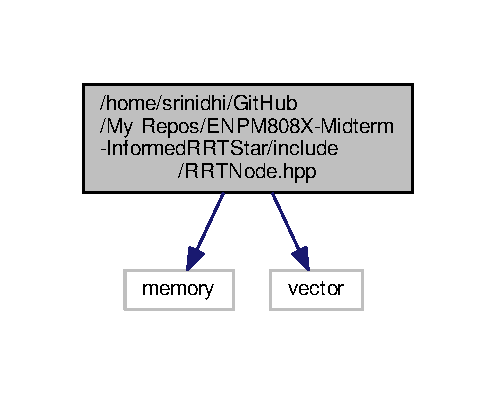
\includegraphics[width=238pt]{RRTNode_8hpp__incl}
\end{center}
\end{figure}
This graph shows which files directly or indirectly include this file\+:
\nopagebreak
\begin{figure}[H]
\begin{center}
\leavevmode
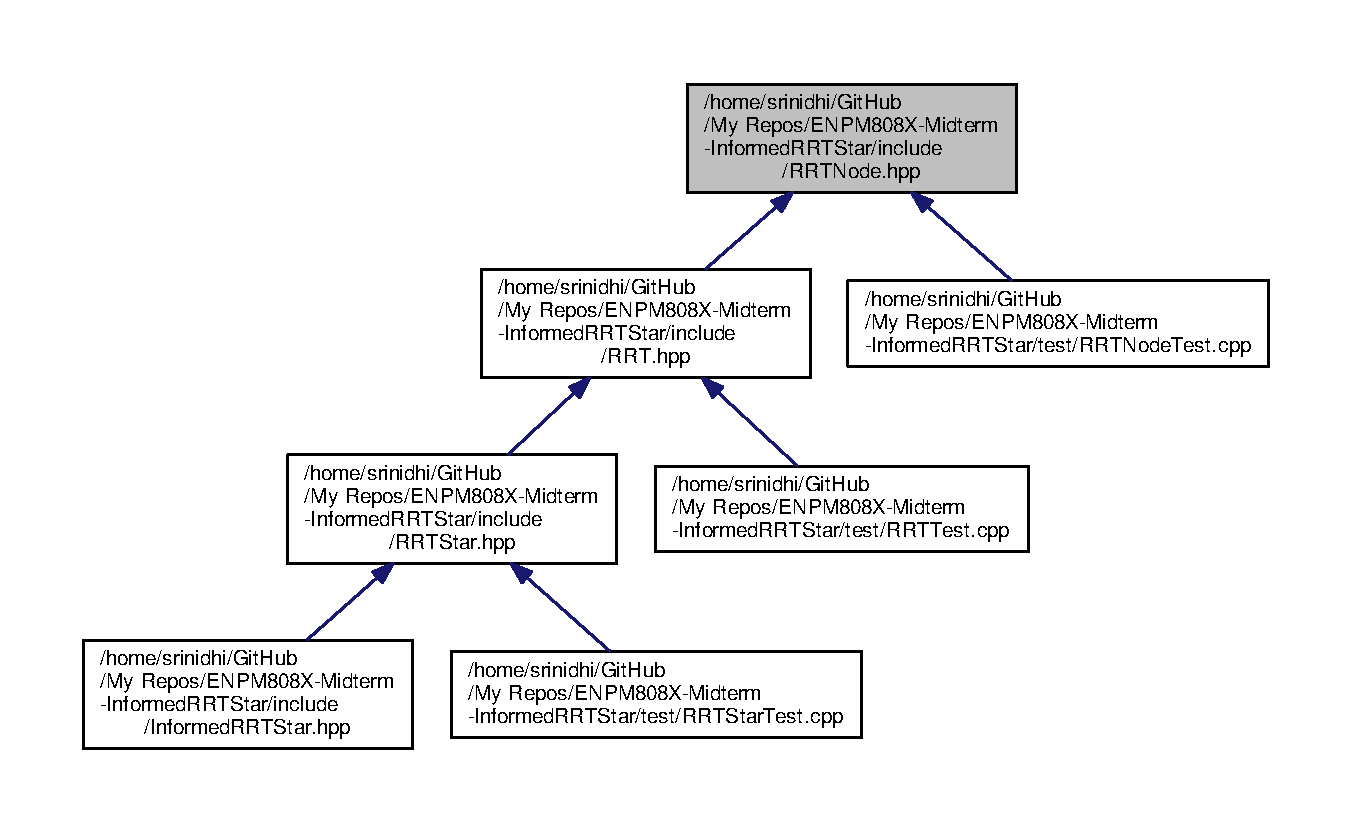
\includegraphics[width=350pt]{RRTNode_8hpp__dep__incl}
\end{center}
\end{figure}
\subsection*{Classes}
\begin{DoxyCompactItemize}
\item 
class \hyperlink{classRRTNode}{R\+R\+T\+Node}
\begin{DoxyCompactList}\small\item\em Class \hyperlink{classRRTNode}{R\+R\+T\+Node} The following class \hyperlink{classRRTNode}{R\+R\+T\+Node} is used to hold information of a node in the tree formed by \hyperlink{classRRT}{R\+RT} algorithm. \end{DoxyCompactList}\end{DoxyCompactItemize}


\subsection{Detailed Description}
\hyperlink{classRRTNode}{R\+R\+T\+Node} class declaration. 

\begin{DoxyAuthor}{Author}
Srinidhi Sreenath (Srinidhi\+Sreenath) 
\end{DoxyAuthor}
\begin{DoxyDate}{Date}
10/10/2018 
\end{DoxyDate}
\begin{DoxyVersion}{Version}
1.\+0
\end{DoxyVersion}
\hypertarget{RRTTest_8cpp_DESCRIPTION}{}\subsection{D\+E\+S\+C\+R\+I\+P\+T\+I\+ON}\label{RRTTest_8cpp_DESCRIPTION}
Header file for class \hyperlink{classRRTNode}{R\+R\+T\+Node}. 
\hypertarget{RRTStar_8hpp}{}\section{/home/srinidhi/\+Git\+Hub/\+My Repos/\+E\+N\+P\+M808\+X-\/\+Midterm-\/\+Informed\+R\+R\+T\+Star/include/\+R\+R\+T\+Star.hpp File Reference}
\label{RRTStar_8hpp}\index{/home/srinidhi/\+Git\+Hub/\+My Repos/\+E\+N\+P\+M808\+X-\/\+Midterm-\/\+Informed\+R\+R\+T\+Star/include/\+R\+R\+T\+Star.\+hpp@{/home/srinidhi/\+Git\+Hub/\+My Repos/\+E\+N\+P\+M808\+X-\/\+Midterm-\/\+Informed\+R\+R\+T\+Star/include/\+R\+R\+T\+Star.\+hpp}}


Informed \hyperlink{classRRT}{R\+RT} Star class declaration.  


{\ttfamily \#include \char`\"{}R\+R\+T.\+hpp\char`\"{}}\\*
Include dependency graph for R\+R\+T\+Star.\+hpp\+:
\nopagebreak
\begin{figure}[H]
\begin{center}
\leavevmode
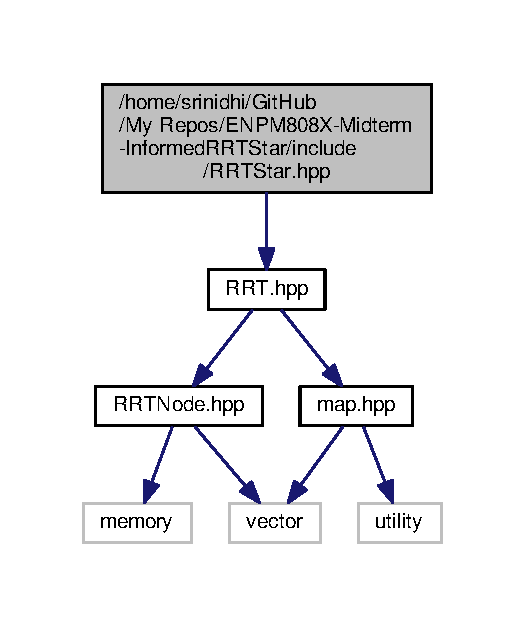
\includegraphics[width=252pt]{RRTStar_8hpp__incl}
\end{center}
\end{figure}
This graph shows which files directly or indirectly include this file\+:
\nopagebreak
\begin{figure}[H]
\begin{center}
\leavevmode
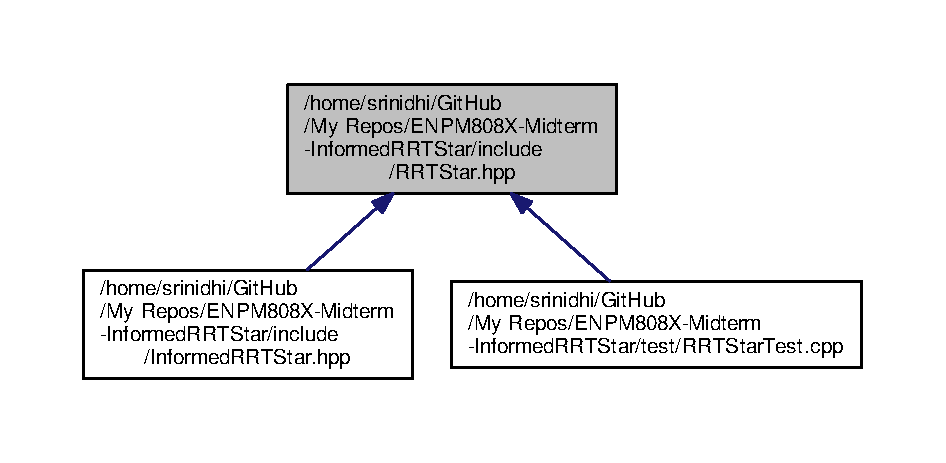
\includegraphics[width=350pt]{RRTStar_8hpp__dep__incl}
\end{center}
\end{figure}
\subsection*{Classes}
\begin{DoxyCompactItemize}
\item 
class \hyperlink{classRRTStar}{R\+R\+T\+Star}
\begin{DoxyCompactList}\small\item\em Class \hyperlink{classRRT}{R\+RT}, derived from class \hyperlink{classRRT}{R\+RT} The following class \hyperlink{classRRT}{R\+RT} Star optimizes the path found by \hyperlink{classRRT}{R\+RT} algorithm using cost to come to rewire the path and the tree nodes as well. \end{DoxyCompactList}\end{DoxyCompactItemize}


\subsection{Detailed Description}
Informed \hyperlink{classRRT}{R\+RT} Star class declaration. 

\hyperlink{classRRT}{R\+RT} Star class declaration.

\begin{DoxyAuthor}{Author}
Srinidhi Sreenath (Srinidhi\+Sreenath) 
\end{DoxyAuthor}
\begin{DoxyDate}{Date}
10/15/2018 
\end{DoxyDate}
\begin{DoxyVersion}{Version}
1.\+0
\end{DoxyVersion}
\hypertarget{RRTTest_8cpp_DESCRIPTION}{}\subsection{D\+E\+S\+C\+R\+I\+P\+T\+I\+ON}\label{RRTTest_8cpp_DESCRIPTION}
Header file for class Informed \hyperlink{classRRT}{R\+RT} Star which implements the Fastly converging Optimized Rapidly-\/exploring Random Tree algorithm to find a path given a map.

\begin{DoxyAuthor}{Author}
Srinidhi Sreenath (Srinidhi\+Sreenath) 
\end{DoxyAuthor}
\begin{DoxyDate}{Date}
10/14/2018 
\end{DoxyDate}
\begin{DoxyVersion}{Version}
1.\+0
\end{DoxyVersion}
\hypertarget{RRTTest_8cpp_DESCRIPTION}{}\subsection{D\+E\+S\+C\+R\+I\+P\+T\+I\+ON}\label{RRTTest_8cpp_DESCRIPTION}
Header file for class \hyperlink{classRRT}{R\+RT} Star which implements the Optimized Rapidly-\/exploring Random Tree algorithm to find a path given a map. 
\hypertarget{main_8cpp}{}\section{/home/srinidhi/\+Git\+Hub/\+My Repos/\+E\+N\+P\+M808\+X-\/\+Midterm-\/\+Informed\+R\+R\+T\+Star/test/main.cpp File Reference}
\label{main_8cpp}\index{/home/srinidhi/\+Git\+Hub/\+My Repos/\+E\+N\+P\+M808\+X-\/\+Midterm-\/\+Informed\+R\+R\+T\+Star/test/main.\+cpp@{/home/srinidhi/\+Git\+Hub/\+My Repos/\+E\+N\+P\+M808\+X-\/\+Midterm-\/\+Informed\+R\+R\+T\+Star/test/main.\+cpp}}


Main file to run all unit tests.  


{\ttfamily \#include $<$gtest/gtest.\+h$>$}\\*
Include dependency graph for main.\+cpp\+:
\nopagebreak
\begin{figure}[H]
\begin{center}
\leavevmode
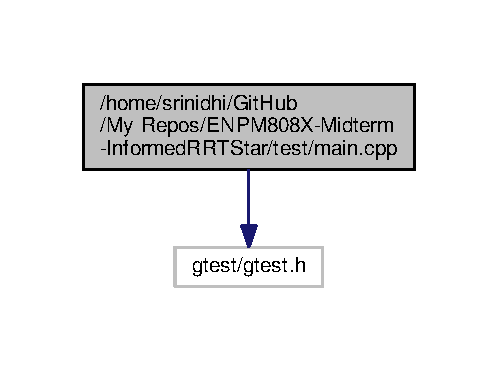
\includegraphics[width=239pt]{main_8cpp__incl}
\end{center}
\end{figure}
\subsection*{Functions}
\begin{DoxyCompactItemize}
\item 
int \hyperlink{main_8cpp_a3c04138a5bfe5d72780bb7e82a18e627}{main} (int argc, char $\ast$$\ast$argv)
\begin{DoxyCompactList}\small\item\em Run all google unit tests. \end{DoxyCompactList}\end{DoxyCompactItemize}


\subsection{Detailed Description}
Main file to run all unit tests. 

\begin{DoxyAuthor}{Author}
Srinidhi Sreenath (Srinidhi\+Sreenath) 
\end{DoxyAuthor}
\begin{DoxyDate}{Date}
10/8/2018 
\end{DoxyDate}
\begin{DoxyVersion}{Version}
1.\+0 
\end{DoxyVersion}


\subsection{Function Documentation}
\index{main.\+cpp@{main.\+cpp}!main@{main}}
\index{main@{main}!main.\+cpp@{main.\+cpp}}
\subsubsection[{\texorpdfstring{main(int argc, char $\ast$$\ast$argv)}{main(int argc, char **argv)}}]{\setlength{\rightskip}{0pt plus 5cm}int main (
\begin{DoxyParamCaption}
\item[{int}]{argc, }
\item[{char $\ast$$\ast$}]{argv}
\end{DoxyParamCaption}
)}\hypertarget{main_8cpp_a3c04138a5bfe5d72780bb7e82a18e627}{}\label{main_8cpp_a3c04138a5bfe5d72780bb7e82a18e627}


Run all google unit tests. 


\begin{DoxyParams}{Parameters}
{\em none} & \\
\hline
\end{DoxyParams}
\begin{DoxyReturn}{Returns}
0 on successful exit 
\end{DoxyReturn}

\hypertarget{MapTest_8cpp}{}\section{/home/srinidhi/\+Git\+Hub/\+My Repos/\+E\+N\+P\+M808\+X-\/\+Midterm-\/\+Informed\+R\+R\+T\+Star/test/\+Map\+Test.cpp File Reference}
\label{MapTest_8cpp}\index{/home/srinidhi/\+Git\+Hub/\+My Repos/\+E\+N\+P\+M808\+X-\/\+Midterm-\/\+Informed\+R\+R\+T\+Star/test/\+Map\+Test.\+cpp@{/home/srinidhi/\+Git\+Hub/\+My Repos/\+E\+N\+P\+M808\+X-\/\+Midterm-\/\+Informed\+R\+R\+T\+Star/test/\+Map\+Test.\+cpp}}


Unit tests for class \hyperlink{classMap}{Map}.  


{\ttfamily \#include $<$gtest/gtest.\+h$>$}\\*
{\ttfamily \#include \char`\"{}map.\+hpp\char`\"{}}\\*
Include dependency graph for Map\+Test.\+cpp\+:
\nopagebreak
\begin{figure}[H]
\begin{center}
\leavevmode
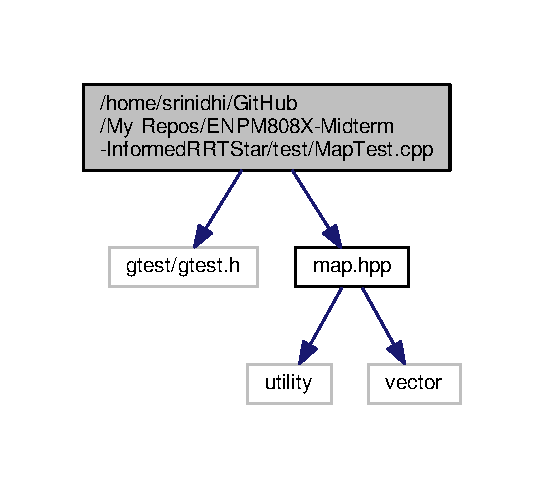
\includegraphics[width=261pt]{MapTest_8cpp__incl}
\end{center}
\end{figure}
\subsection*{Functions}
\begin{DoxyCompactItemize}
\item 
\hyperlink{MapTest_8cpp_af2cc01b31d84350d76e842fe906f9c26}{T\+E\+ST} (Map\+Initialization\+Test1, test\+Set\+Map\+Workspace\+Boundary)
\begin{DoxyCompactList}\small\item\em Test case to check setting workspace boundary. \end{DoxyCompactList}\item 
\hyperlink{MapTest_8cpp_a3de69499ba2b105cf0b61d4a72489fd8}{T\+E\+ST} (Map\+Initialization\+Test2, test\+Add\+Obsatcles\+To\+Map)
\begin{DoxyCompactList}\small\item\em Test case to check setting obstacles. \end{DoxyCompactList}\item 
\hyperlink{MapTest_8cpp_a536f73731ed841aeb7d34ad791c57a14}{T\+E\+ST} (Map\+Valid\+Node\+Test1, test\+Valid\+Node\+Based\+On\+Boundary)
\begin{DoxyCompactList}\small\item\em Test case to check is\+Outof\+Map member function output based on input node. \end{DoxyCompactList}\item 
\hyperlink{MapTest_8cpp_a870a7b0e1d38c9e572e68a5b29a99d2e}{T\+E\+ST} (Map\+Valid\+Node\+Test2, test\+Valid\+Connection\+To\+Tree\+Node)
\begin{DoxyCompactList}\small\item\em Test case to check is\+Valid\+Node member function output based on input node. \end{DoxyCompactList}\item 
\hyperlink{MapTest_8cpp_a379a61468326f6a5e60eefeb87c20c84}{T\+E\+ST} (Map\+Reset\+Test, test\+Map\+Reset\+Function)
\begin{DoxyCompactList}\small\item\em Test case to check resetting map. \end{DoxyCompactList}\end{DoxyCompactItemize}
\subsection*{Variables}
\begin{DoxyCompactItemize}
\item 
\hyperlink{classMap}{Map} \hyperlink{MapTest_8cpp_a5c84b62dfdeebcc95f6344dbccff893b}{sample\+Map}\hypertarget{MapTest_8cpp_a5c84b62dfdeebcc95f6344dbccff893b}{}\label{MapTest_8cpp_a5c84b62dfdeebcc95f6344dbccff893b}

\begin{DoxyCompactList}\small\item\em class object \end{DoxyCompactList}\item 
std\+::vector$<$ std\+::pair$<$ double, double $>$ $>$ \hyperlink{MapTest_8cpp_ad2559d9d65caf07bc831e905bc151444}{boundary}\hypertarget{MapTest_8cpp_ad2559d9d65caf07bc831e905bc151444}{}\label{MapTest_8cpp_ad2559d9d65caf07bc831e905bc151444}

\begin{DoxyCompactList}\small\item\em variable to hold boundary vertices \end{DoxyCompactList}\item 
std\+::vector$<$ std\+::vector$<$ double $>$ $>$ \hyperlink{MapTest_8cpp_ab66426f62219d5ce7554221a370691fe}{obstacles}\hypertarget{MapTest_8cpp_ab66426f62219d5ce7554221a370691fe}{}\label{MapTest_8cpp_ab66426f62219d5ce7554221a370691fe}

\begin{DoxyCompactList}\small\item\em variable to hold obstacles and their vertices \end{DoxyCompactList}\end{DoxyCompactItemize}


\subsection{Detailed Description}
Unit tests for class \hyperlink{classMap}{Map}. 

\begin{DoxyAuthor}{Author}
Srinidhi Sreenath (Srinidhi\+Sreenath) 
\end{DoxyAuthor}
\begin{DoxyDate}{Date}
10/8/2018 
\end{DoxyDate}
\begin{DoxyVersion}{Version}
1.\+0
\end{DoxyVersion}
\hypertarget{RRTTest_8cpp_DESCRIPTION}{}\subsection{D\+E\+S\+C\+R\+I\+P\+T\+I\+ON}\label{RRTTest_8cpp_DESCRIPTION}
Test cases to test member functions of class \hyperlink{classMap}{Map}. 

\subsection{Function Documentation}
\index{Map\+Test.\+cpp@{Map\+Test.\+cpp}!T\+E\+ST@{T\+E\+ST}}
\index{T\+E\+ST@{T\+E\+ST}!Map\+Test.\+cpp@{Map\+Test.\+cpp}}
\subsubsection[{\texorpdfstring{T\+E\+S\+T(\+Map\+Initialization\+Test1, test\+Set\+Map\+Workspace\+Boundary)}{TEST(MapInitializationTest1, testSetMapWorkspaceBoundary)}}]{\setlength{\rightskip}{0pt plus 5cm}T\+E\+ST (
\begin{DoxyParamCaption}
\item[{Map\+Initialization\+Test1}]{, }
\item[{test\+Set\+Map\+Workspace\+Boundary}]{}
\end{DoxyParamCaption}
)}\hypertarget{MapTest_8cpp_af2cc01b31d84350d76e842fe906f9c26}{}\label{MapTest_8cpp_af2cc01b31d84350d76e842fe906f9c26}


Test case to check setting workspace boundary. 


\begin{DoxyParams}{Parameters}
{\em none} & \\
\hline
\end{DoxyParams}
\begin{DoxyReturn}{Returns}
none 
\end{DoxyReturn}
\index{Map\+Test.\+cpp@{Map\+Test.\+cpp}!T\+E\+ST@{T\+E\+ST}}
\index{T\+E\+ST@{T\+E\+ST}!Map\+Test.\+cpp@{Map\+Test.\+cpp}}
\subsubsection[{\texorpdfstring{T\+E\+S\+T(\+Map\+Initialization\+Test2, test\+Add\+Obsatcles\+To\+Map)}{TEST(MapInitializationTest2, testAddObsatclesToMap)}}]{\setlength{\rightskip}{0pt plus 5cm}T\+E\+ST (
\begin{DoxyParamCaption}
\item[{Map\+Initialization\+Test2}]{, }
\item[{test\+Add\+Obsatcles\+To\+Map}]{}
\end{DoxyParamCaption}
)}\hypertarget{MapTest_8cpp_a3de69499ba2b105cf0b61d4a72489fd8}{}\label{MapTest_8cpp_a3de69499ba2b105cf0b61d4a72489fd8}


Test case to check setting obstacles. 


\begin{DoxyParams}{Parameters}
{\em none} & \\
\hline
\end{DoxyParams}
\begin{DoxyReturn}{Returns}
none 
\end{DoxyReturn}
\index{Map\+Test.\+cpp@{Map\+Test.\+cpp}!T\+E\+ST@{T\+E\+ST}}
\index{T\+E\+ST@{T\+E\+ST}!Map\+Test.\+cpp@{Map\+Test.\+cpp}}
\subsubsection[{\texorpdfstring{T\+E\+S\+T(\+Map\+Valid\+Node\+Test1, test\+Valid\+Node\+Based\+On\+Boundary)}{TEST(MapValidNodeTest1, testValidNodeBasedOnBoundary)}}]{\setlength{\rightskip}{0pt plus 5cm}T\+E\+ST (
\begin{DoxyParamCaption}
\item[{Map\+Valid\+Node\+Test1}]{, }
\item[{test\+Valid\+Node\+Based\+On\+Boundary}]{}
\end{DoxyParamCaption}
)}\hypertarget{MapTest_8cpp_a536f73731ed841aeb7d34ad791c57a14}{}\label{MapTest_8cpp_a536f73731ed841aeb7d34ad791c57a14}


Test case to check is\+Outof\+Map member function output based on input node. 


\begin{DoxyParams}{Parameters}
{\em none} & \\
\hline
\end{DoxyParams}
\begin{DoxyReturn}{Returns}
none 
\end{DoxyReturn}
$<$ sample node within boundary

$<$ sample node outside boundary \index{Map\+Test.\+cpp@{Map\+Test.\+cpp}!T\+E\+ST@{T\+E\+ST}}
\index{T\+E\+ST@{T\+E\+ST}!Map\+Test.\+cpp@{Map\+Test.\+cpp}}
\subsubsection[{\texorpdfstring{T\+E\+S\+T(\+Map\+Valid\+Node\+Test2, test\+Valid\+Connection\+To\+Tree\+Node)}{TEST(MapValidNodeTest2, testValidConnectionToTreeNode)}}]{\setlength{\rightskip}{0pt plus 5cm}T\+E\+ST (
\begin{DoxyParamCaption}
\item[{Map\+Valid\+Node\+Test2}]{, }
\item[{test\+Valid\+Connection\+To\+Tree\+Node}]{}
\end{DoxyParamCaption}
)}\hypertarget{MapTest_8cpp_a870a7b0e1d38c9e572e68a5b29a99d2e}{}\label{MapTest_8cpp_a870a7b0e1d38c9e572e68a5b29a99d2e}


Test case to check is\+Valid\+Node member function output based on input node. 


\begin{DoxyParams}{Parameters}
{\em none} & \\
\hline
\end{DoxyParams}
\begin{DoxyReturn}{Returns}
none 
\end{DoxyReturn}
\index{Map\+Test.\+cpp@{Map\+Test.\+cpp}!T\+E\+ST@{T\+E\+ST}}
\index{T\+E\+ST@{T\+E\+ST}!Map\+Test.\+cpp@{Map\+Test.\+cpp}}
\subsubsection[{\texorpdfstring{T\+E\+S\+T(\+Map\+Reset\+Test, test\+Map\+Reset\+Function)}{TEST(MapResetTest, testMapResetFunction)}}]{\setlength{\rightskip}{0pt plus 5cm}T\+E\+ST (
\begin{DoxyParamCaption}
\item[{Map\+Reset\+Test}]{, }
\item[{test\+Map\+Reset\+Function}]{}
\end{DoxyParamCaption}
)}\hypertarget{MapTest_8cpp_a379a61468326f6a5e60eefeb87c20c84}{}\label{MapTest_8cpp_a379a61468326f6a5e60eefeb87c20c84}


Test case to check resetting map. 


\begin{DoxyParams}{Parameters}
{\em none} & \\
\hline
\end{DoxyParams}
\begin{DoxyReturn}{Returns}
none 
\end{DoxyReturn}
$<$ unsigned variable to compare sizes 
\hypertarget{RRTNodeTest_8cpp}{}\section{/home/srinidhi/\+Git\+Hub/\+My Repos/\+E\+N\+P\+M808\+X-\/\+Midterm-\/\+Informed\+R\+R\+T\+Star/test/\+R\+R\+T\+Node\+Test.cpp File Reference}
\label{RRTNodeTest_8cpp}\index{/home/srinidhi/\+Git\+Hub/\+My Repos/\+E\+N\+P\+M808\+X-\/\+Midterm-\/\+Informed\+R\+R\+T\+Star/test/\+R\+R\+T\+Node\+Test.\+cpp@{/home/srinidhi/\+Git\+Hub/\+My Repos/\+E\+N\+P\+M808\+X-\/\+Midterm-\/\+Informed\+R\+R\+T\+Star/test/\+R\+R\+T\+Node\+Test.\+cpp}}


Unit tests for class \hyperlink{classRRTNode}{R\+R\+T\+Node}.  


{\ttfamily \#include $<$gtest/gtest.\+h$>$}\\*
{\ttfamily \#include \char`\"{}R\+R\+T\+Node.\+hpp\char`\"{}}\\*
Include dependency graph for R\+R\+T\+Node\+Test.\+cpp\+:
\nopagebreak
\begin{figure}[H]
\begin{center}
\leavevmode
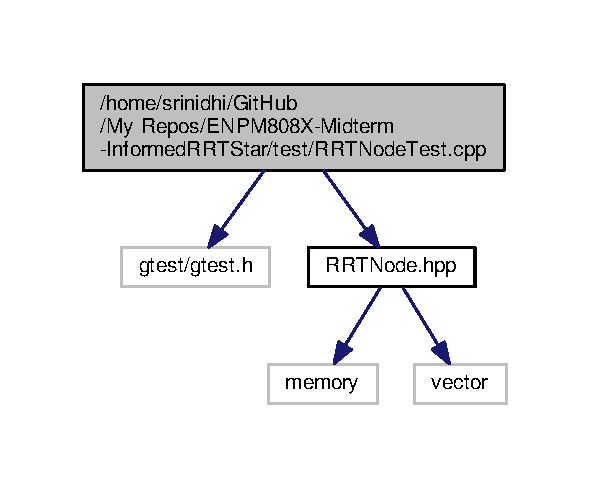
\includegraphics[width=283pt]{RRTNodeTest_8cpp__incl}
\end{center}
\end{figure}
\subsection*{Functions}
\begin{DoxyCompactItemize}
\item 
\hyperlink{RRTNodeTest_8cpp_a647b8a10a5a65449a3ff1d799019d7be}{T\+E\+ST} (R\+R\+T\+Node\+Set\+State\+Test, test\+Set\+State\+Of\+R\+R\+T\+Node)
\begin{DoxyCompactList}\small\item\em Test case to check setting state of \hyperlink{classRRTNode}{R\+R\+T\+Node}. \end{DoxyCompactList}\item 
\hyperlink{RRTNodeTest_8cpp_a8281619788f60d2e74b7a42aedb7747f}{T\+E\+ST} (R\+R\+T\+Node\+Set\+Parent\+Node\+Test, test\+Set\+Parent\+Of\+Current\+R\+R\+T\+Node)
\begin{DoxyCompactList}\small\item\em Test case to check setting parent node for current node. \end{DoxyCompactList}\item 
\hyperlink{RRTNodeTest_8cpp_a554d25380e7aff63559a0ae01e80e177}{T\+E\+ST} (R\+R\+T\+Node\+Change\+Parent\+Node\+Test, test\+Set\+New\+Parent\+For\+Current\+R\+R\+T\+Node)
\begin{DoxyCompactList}\small\item\em Test case to check changing parent node for current node. \end{DoxyCompactList}\item 
\hyperlink{RRTNodeTest_8cpp_ab0b090423f26e758486319565bde44fe}{T\+E\+ST} (R\+R\+T\+Node\+Set\+Cost\+To\+Come, test\+Cost\+To\+Come\+For\+Current\+Node)
\begin{DoxyCompactList}\small\item\em Test case to check setting cost to come for current node. \end{DoxyCompactList}\end{DoxyCompactItemize}


\subsection{Detailed Description}
Unit tests for class \hyperlink{classRRTNode}{R\+R\+T\+Node}. 

\begin{DoxyAuthor}{Author}
Srinidhi Sreenath (Srinidhi\+Sreenath) 
\end{DoxyAuthor}
\begin{DoxyDate}{Date}
10/10/2018 
\end{DoxyDate}
\begin{DoxyVersion}{Version}
1.\+0
\end{DoxyVersion}
\hypertarget{RRTTest_8cpp_DESCRIPTION}{}\subsection{D\+E\+S\+C\+R\+I\+P\+T\+I\+ON}\label{RRTTest_8cpp_DESCRIPTION}
Test cases to test member functions of class \hyperlink{classRRTNode}{R\+R\+T\+Node}. 

\subsection{Function Documentation}
\index{R\+R\+T\+Node\+Test.\+cpp@{R\+R\+T\+Node\+Test.\+cpp}!T\+E\+ST@{T\+E\+ST}}
\index{T\+E\+ST@{T\+E\+ST}!R\+R\+T\+Node\+Test.\+cpp@{R\+R\+T\+Node\+Test.\+cpp}}
\subsubsection[{\texorpdfstring{T\+E\+S\+T(\+R\+R\+T\+Node\+Set\+State\+Test, test\+Set\+State\+Of\+R\+R\+T\+Node)}{TEST(RRTNodeSetStateTest, testSetStateOfRRTNode)}}]{\setlength{\rightskip}{0pt plus 5cm}T\+E\+ST (
\begin{DoxyParamCaption}
\item[{R\+R\+T\+Node\+Set\+State\+Test}]{, }
\item[{test\+Set\+State\+Of\+R\+R\+T\+Node}]{}
\end{DoxyParamCaption}
)}\hypertarget{RRTNodeTest_8cpp_a647b8a10a5a65449a3ff1d799019d7be}{}\label{RRTNodeTest_8cpp_a647b8a10a5a65449a3ff1d799019d7be}


Test case to check setting state of \hyperlink{classRRTNode}{R\+R\+T\+Node}. 


\begin{DoxyParams}{Parameters}
{\em none} & \\
\hline
\end{DoxyParams}
\begin{DoxyReturn}{Returns}
none 
\end{DoxyReturn}
\index{R\+R\+T\+Node\+Test.\+cpp@{R\+R\+T\+Node\+Test.\+cpp}!T\+E\+ST@{T\+E\+ST}}
\index{T\+E\+ST@{T\+E\+ST}!R\+R\+T\+Node\+Test.\+cpp@{R\+R\+T\+Node\+Test.\+cpp}}
\subsubsection[{\texorpdfstring{T\+E\+S\+T(\+R\+R\+T\+Node\+Set\+Parent\+Node\+Test, test\+Set\+Parent\+Of\+Current\+R\+R\+T\+Node)}{TEST(RRTNodeSetParentNodeTest, testSetParentOfCurrentRRTNode)}}]{\setlength{\rightskip}{0pt plus 5cm}T\+E\+ST (
\begin{DoxyParamCaption}
\item[{R\+R\+T\+Node\+Set\+Parent\+Node\+Test}]{, }
\item[{test\+Set\+Parent\+Of\+Current\+R\+R\+T\+Node}]{}
\end{DoxyParamCaption}
)}\hypertarget{RRTNodeTest_8cpp_a8281619788f60d2e74b7a42aedb7747f}{}\label{RRTNodeTest_8cpp_a8281619788f60d2e74b7a42aedb7747f}


Test case to check setting parent node for current node. 


\begin{DoxyParams}{Parameters}
{\em none} & \\
\hline
\end{DoxyParams}
\begin{DoxyReturn}{Returns}
none 
\end{DoxyReturn}
\index{R\+R\+T\+Node\+Test.\+cpp@{R\+R\+T\+Node\+Test.\+cpp}!T\+E\+ST@{T\+E\+ST}}
\index{T\+E\+ST@{T\+E\+ST}!R\+R\+T\+Node\+Test.\+cpp@{R\+R\+T\+Node\+Test.\+cpp}}
\subsubsection[{\texorpdfstring{T\+E\+S\+T(\+R\+R\+T\+Node\+Change\+Parent\+Node\+Test, test\+Set\+New\+Parent\+For\+Current\+R\+R\+T\+Node)}{TEST(RRTNodeChangeParentNodeTest, testSetNewParentForCurrentRRTNode)}}]{\setlength{\rightskip}{0pt plus 5cm}T\+E\+ST (
\begin{DoxyParamCaption}
\item[{R\+R\+T\+Node\+Change\+Parent\+Node\+Test}]{, }
\item[{test\+Set\+New\+Parent\+For\+Current\+R\+R\+T\+Node}]{}
\end{DoxyParamCaption}
)}\hypertarget{RRTNodeTest_8cpp_a554d25380e7aff63559a0ae01e80e177}{}\label{RRTNodeTest_8cpp_a554d25380e7aff63559a0ae01e80e177}


Test case to check changing parent node for current node. 


\begin{DoxyParams}{Parameters}
{\em none} & \\
\hline
\end{DoxyParams}
\begin{DoxyReturn}{Returns}
none 
\end{DoxyReturn}
\index{R\+R\+T\+Node\+Test.\+cpp@{R\+R\+T\+Node\+Test.\+cpp}!T\+E\+ST@{T\+E\+ST}}
\index{T\+E\+ST@{T\+E\+ST}!R\+R\+T\+Node\+Test.\+cpp@{R\+R\+T\+Node\+Test.\+cpp}}
\subsubsection[{\texorpdfstring{T\+E\+S\+T(\+R\+R\+T\+Node\+Set\+Cost\+To\+Come, test\+Cost\+To\+Come\+For\+Current\+Node)}{TEST(RRTNodeSetCostToCome, testCostToComeForCurrentNode)}}]{\setlength{\rightskip}{0pt plus 5cm}T\+E\+ST (
\begin{DoxyParamCaption}
\item[{R\+R\+T\+Node\+Set\+Cost\+To\+Come}]{, }
\item[{test\+Cost\+To\+Come\+For\+Current\+Node}]{}
\end{DoxyParamCaption}
)}\hypertarget{RRTNodeTest_8cpp_ab0b090423f26e758486319565bde44fe}{}\label{RRTNodeTest_8cpp_ab0b090423f26e758486319565bde44fe}


Test case to check setting cost to come for current node. 


\begin{DoxyParams}{Parameters}
{\em none} & \\
\hline
\end{DoxyParams}
\begin{DoxyReturn}{Returns}
none 
\end{DoxyReturn}

\hypertarget{RRTStarTest_8cpp}{}\section{/home/srinidhi/\+Git\+Hub/\+My Repos/\+E\+N\+P\+M808\+X-\/\+Midterm-\/\+Informed\+R\+R\+T\+Star/test/\+R\+R\+T\+Star\+Test.cpp File Reference}
\label{RRTStarTest_8cpp}\index{/home/srinidhi/\+Git\+Hub/\+My Repos/\+E\+N\+P\+M808\+X-\/\+Midterm-\/\+Informed\+R\+R\+T\+Star/test/\+R\+R\+T\+Star\+Test.\+cpp@{/home/srinidhi/\+Git\+Hub/\+My Repos/\+E\+N\+P\+M808\+X-\/\+Midterm-\/\+Informed\+R\+R\+T\+Star/test/\+R\+R\+T\+Star\+Test.\+cpp}}


Unit tests for class \hyperlink{classRRT}{R\+RT}.  


{\ttfamily \#include $<$gtest/gtest.\+h$>$}\\*
{\ttfamily \#include $<$cmath$>$}\\*
{\ttfamily \#include \char`\"{}R\+R\+T\+Star.\+hpp\char`\"{}}\\*
Include dependency graph for R\+R\+T\+Star\+Test.\+cpp\+:
\nopagebreak
\begin{figure}[H]
\begin{center}
\leavevmode
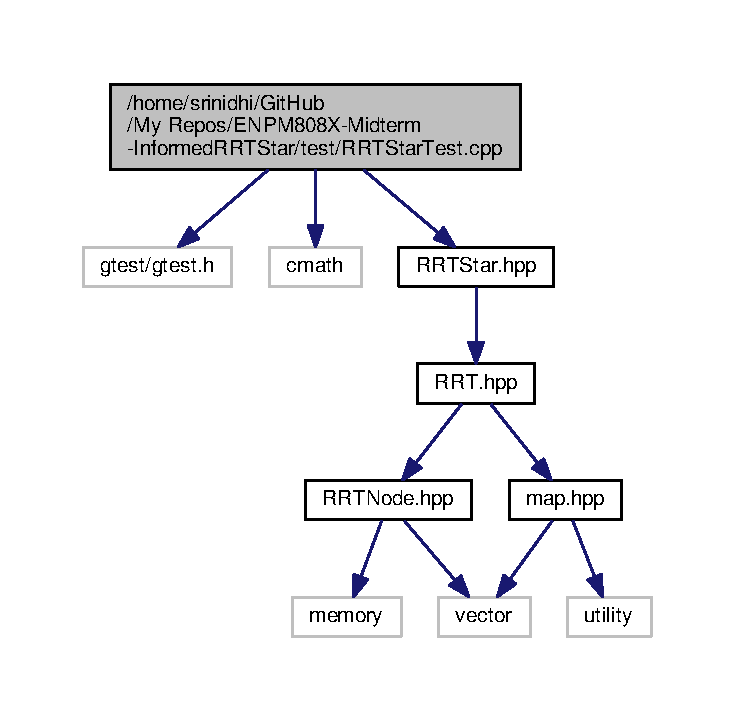
\includegraphics[width=350pt]{RRTStarTest_8cpp__incl}
\end{center}
\end{figure}
\subsection*{Functions}
\begin{DoxyCompactItemize}
\item 
\hyperlink{RRTStarTest_8cpp_a58aa89533582f4016ec61ec168467082}{T\+E\+ST} (R\+R\+T\+Star\+Valid\+Path\+Test, test\+Validity\+Of\+Path\+Given\+By\+The\+R\+R\+T\+Star\+Planner)
\begin{DoxyCompactList}\small\item\em Test case to check the \hyperlink{classRRT}{R\+RT} Star planner. The test case checks whether the path found is correct based on the following three conditions\+: \end{DoxyCompactList}\item 
{\bfseries T\+E\+ST} (R\+R\+T\+Star\+Planner\+Reset\+Test, test\+R\+R\+T\+Star\+Reset\+Function)\hypertarget{RRTStarTest_8cpp_aa5c415a782a7869bf80c9f277dda1932}{}\label{RRTStarTest_8cpp_aa5c415a782a7869bf80c9f277dda1932}

\end{DoxyCompactItemize}
\subsection*{Variables}
\begin{DoxyCompactItemize}
\item 
\hyperlink{classRRTStar}{R\+R\+T\+Star} \hyperlink{RRTStarTest_8cpp_a07af0769372e0a44f11b0563caffabe4}{sample\+Plan}
\begin{DoxyCompactList}\small\item\em Initialize Test planner. \end{DoxyCompactList}\item 
std\+::vector$<$ std\+::pair$<$ double, double $>$ $>$ \hyperlink{RRTStarTest_8cpp_aad7540fdc75806d8b12e2771e211377f}{sample\+Boundary}\hypertarget{RRTStarTest_8cpp_aad7540fdc75806d8b12e2771e211377f}{}\label{RRTStarTest_8cpp_aad7540fdc75806d8b12e2771e211377f}

\begin{DoxyCompactList}\small\item\em variable to hold boundary vertices \end{DoxyCompactList}\item 
std\+::vector$<$ std\+::vector$<$ double $>$ $>$ \hyperlink{RRTStarTest_8cpp_aa8cc35576c8ac9c1d2e8e3542edabd2b}{sample\+Obstacles}\hypertarget{RRTStarTest_8cpp_aa8cc35576c8ac9c1d2e8e3542edabd2b}{}\label{RRTStarTest_8cpp_aa8cc35576c8ac9c1d2e8e3542edabd2b}

\begin{DoxyCompactList}\small\item\em variable to hold obstacles and their vertices \end{DoxyCompactList}\end{DoxyCompactItemize}


\subsection{Detailed Description}
Unit tests for class \hyperlink{classRRT}{R\+RT}. 

\begin{DoxyAuthor}{Author}
Srinidhi Sreenath (Srinidhi\+Sreenath) 
\end{DoxyAuthor}
\begin{DoxyDate}{Date}
10/15/2018 
\end{DoxyDate}
\begin{DoxyVersion}{Version}
1.\+0
\end{DoxyVersion}
\hypertarget{RRTTest_8cpp_DESCRIPTION}{}\subsection{D\+E\+S\+C\+R\+I\+P\+T\+I\+ON}\label{RRTTest_8cpp_DESCRIPTION}
Test cases to test the class members of Informed \hyperlink{classRRT}{R\+RT} Star planner.

\begin{DoxyAuthor}{Author}
Srinidhi Sreenath (Srinidhi\+Sreenath) 
\end{DoxyAuthor}
\begin{DoxyDate}{Date}
10/14/2018 
\end{DoxyDate}
\begin{DoxyVersion}{Version}
1.\+0
\end{DoxyVersion}
\hypertarget{RRTTest_8cpp_DESCRIPTION}{}\subsection{D\+E\+S\+C\+R\+I\+P\+T\+I\+ON}\label{RRTTest_8cpp_DESCRIPTION}
Test cases to test the class members of \hyperlink{classRRT}{R\+RT} Star planner. 

\subsection{Function Documentation}
\index{R\+R\+T\+Star\+Test.\+cpp@{R\+R\+T\+Star\+Test.\+cpp}!T\+E\+ST@{T\+E\+ST}}
\index{T\+E\+ST@{T\+E\+ST}!R\+R\+T\+Star\+Test.\+cpp@{R\+R\+T\+Star\+Test.\+cpp}}
\subsubsection[{\texorpdfstring{T\+E\+S\+T(\+R\+R\+T\+Star\+Valid\+Path\+Test, test\+Validity\+Of\+Path\+Given\+By\+The\+R\+R\+T\+Star\+Planner)}{TEST(RRTStarValidPathTest, testValidityOfPathGivenByTheRRTStarPlanner)}}]{\setlength{\rightskip}{0pt plus 5cm}T\+E\+ST (
\begin{DoxyParamCaption}
\item[{R\+R\+T\+Star\+Valid\+Path\+Test}]{, }
\item[{test\+Validity\+Of\+Path\+Given\+By\+The\+R\+R\+T\+Star\+Planner}]{}
\end{DoxyParamCaption}
)}\hypertarget{RRTStarTest_8cpp_a58aa89533582f4016ec61ec168467082}{}\label{RRTStarTest_8cpp_a58aa89533582f4016ec61ec168467082}


Test case to check the \hyperlink{classRRT}{R\+RT} Star planner. The test case checks whether the path found is correct based on the following three conditions\+: 


\begin{DoxyEnumerate}
\item The last waypoint of the path should be the goal node. (i.\+e the goal node is a leaf node in the R\+R\+Tree)
\item Tracing the parent of the goal node in the tree, the path should end at the start node i.\+e root node
\item The distance between each waypoint should be within drivable range of the planner
\end{DoxyEnumerate}


\begin{DoxyParams}{Parameters}
{\em none} & \\
\hline
\end{DoxyParams}
\begin{DoxyReturn}{Returns}
none 
\end{DoxyReturn}


\subsection{Variable Documentation}
\index{R\+R\+T\+Star\+Test.\+cpp@{R\+R\+T\+Star\+Test.\+cpp}!sample\+Plan@{sample\+Plan}}
\index{sample\+Plan@{sample\+Plan}!R\+R\+T\+Star\+Test.\+cpp@{R\+R\+T\+Star\+Test.\+cpp}}
\subsubsection[{\texorpdfstring{sample\+Plan}{samplePlan}}]{\setlength{\rightskip}{0pt plus 5cm}{\bf R\+R\+T\+Star} sample\+Plan}\hypertarget{RRTStarTest_8cpp_a07af0769372e0a44f11b0563caffabe4}{}\label{RRTStarTest_8cpp_a07af0769372e0a44f11b0563caffabe4}


Initialize Test planner. 

The following test cases follow similar test cases to class \hyperlink{classRRT}{R\+RT}. Due to the probabilistic nature of the algorithm, a test case to check for optimality cannot pass all the time. Optimality depends on certain factors like max number of iterations, the environment, start and end points etc.

A test case to check for optimality is not currently implemented due to the non deterministic behavior. 
\hypertarget{RRTTest_8cpp}{}\section{/home/srinidhi/\+Git\+Hub/\+My Repos/\+E\+N\+P\+M808\+X-\/\+Midterm-\/\+Informed\+R\+R\+T\+Star/test/\+R\+R\+T\+Test.cpp File Reference}
\label{RRTTest_8cpp}\index{/home/srinidhi/\+Git\+Hub/\+My Repos/\+E\+N\+P\+M808\+X-\/\+Midterm-\/\+Informed\+R\+R\+T\+Star/test/\+R\+R\+T\+Test.\+cpp@{/home/srinidhi/\+Git\+Hub/\+My Repos/\+E\+N\+P\+M808\+X-\/\+Midterm-\/\+Informed\+R\+R\+T\+Star/test/\+R\+R\+T\+Test.\+cpp}}


Unit tests for class \hyperlink{classRRT}{R\+RT}.  


{\ttfamily \#include $<$gtest/gtest.\+h$>$}\\*
{\ttfamily \#include $<$cmath$>$}\\*
{\ttfamily \#include \char`\"{}R\+R\+T.\+hpp\char`\"{}}\\*
Include dependency graph for R\+R\+T\+Test.\+cpp\+:
\nopagebreak
\begin{figure}[H]
\begin{center}
\leavevmode
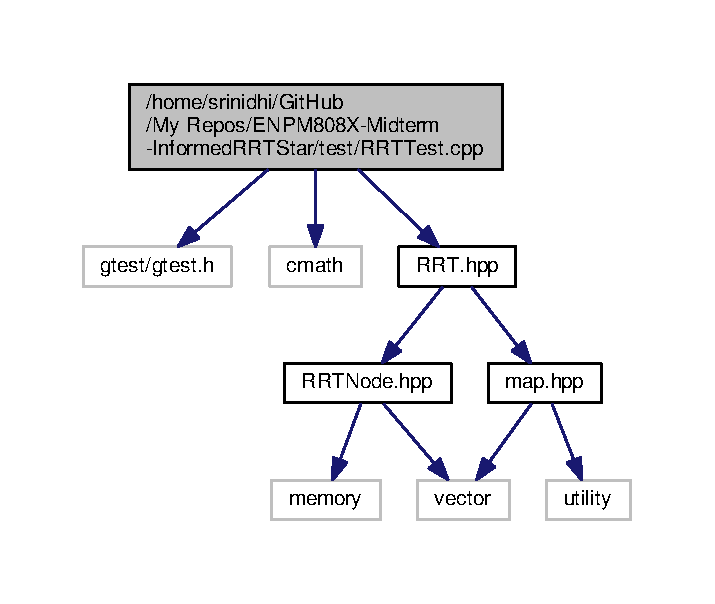
\includegraphics[width=343pt]{RRTTest_8cpp__incl}
\end{center}
\end{figure}
\subsection*{Functions}
\begin{DoxyCompactItemize}
\item 
\hyperlink{RRTTest_8cpp_a41d9096b6c18bdea63f68836223c766d}{T\+E\+ST} (R\+R\+T\+Valid\+Path\+Test, test\+Validity\+Of\+Path\+Given\+By\+The\+R\+R\+T\+Planner)
\begin{DoxyCompactList}\small\item\em Test case to check the \hyperlink{classRRT}{R\+RT} planner. The test case checks whether the path found is correct based on the following three conditions\+: \end{DoxyCompactList}\item 
{\bfseries T\+E\+ST} (R\+R\+T\+Planner\+Reset\+Test, test\+R\+R\+T\+Reset\+Function)\hypertarget{RRTTest_8cpp_a4c3e1f3bfcef8286f2e021e22e0bb48a}{}\label{RRTTest_8cpp_a4c3e1f3bfcef8286f2e021e22e0bb48a}

\end{DoxyCompactItemize}
\subsection*{Variables}
\begin{DoxyCompactItemize}
\item 
\hyperlink{classRRT}{R\+RT} \hyperlink{RRTTest_8cpp_a39f825702d1861c4cf1b2810c9497231}{test\+Plan}\hypertarget{RRTTest_8cpp_a39f825702d1861c4cf1b2810c9497231}{}\label{RRTTest_8cpp_a39f825702d1861c4cf1b2810c9497231}

\begin{DoxyCompactList}\small\item\em Initialize Test planner. \end{DoxyCompactList}\item 
std\+::vector$<$ std\+::pair$<$ double, double $>$ $>$ \hyperlink{RRTTest_8cpp_a95c04c5421f1ce2f9506c71f8757a1e6}{test\+Boundary}\hypertarget{RRTTest_8cpp_a95c04c5421f1ce2f9506c71f8757a1e6}{}\label{RRTTest_8cpp_a95c04c5421f1ce2f9506c71f8757a1e6}

\begin{DoxyCompactList}\small\item\em variable to hold boundary vertices \end{DoxyCompactList}\item 
std\+::vector$<$ std\+::vector$<$ double $>$ $>$ \hyperlink{RRTTest_8cpp_ae79b830cfb3725148a4ad66fb38764c7}{test\+Obstacles}\hypertarget{RRTTest_8cpp_ae79b830cfb3725148a4ad66fb38764c7}{}\label{RRTTest_8cpp_ae79b830cfb3725148a4ad66fb38764c7}

\begin{DoxyCompactList}\small\item\em variable to hold obstacles and their vertices \end{DoxyCompactList}\end{DoxyCompactItemize}


\subsection{Detailed Description}
Unit tests for class \hyperlink{classRRT}{R\+RT}. 

\begin{DoxyAuthor}{Author}
Srinidhi Sreenath (Srinidhi\+Sreenath) 
\end{DoxyAuthor}
\begin{DoxyDate}{Date}
10/13/2018 
\end{DoxyDate}
\begin{DoxyVersion}{Version}
1.\+0
\end{DoxyVersion}
\hypertarget{RRTTest_8cpp_DESCRIPTION}{}\subsection{D\+E\+S\+C\+R\+I\+P\+T\+I\+ON}\label{RRTTest_8cpp_DESCRIPTION}
Test cases to test the class members of \hyperlink{classRRT}{R\+RT} planner. 

\subsection{Function Documentation}
\index{R\+R\+T\+Test.\+cpp@{R\+R\+T\+Test.\+cpp}!T\+E\+ST@{T\+E\+ST}}
\index{T\+E\+ST@{T\+E\+ST}!R\+R\+T\+Test.\+cpp@{R\+R\+T\+Test.\+cpp}}
\subsubsection[{\texorpdfstring{T\+E\+S\+T(\+R\+R\+T\+Valid\+Path\+Test, test\+Validity\+Of\+Path\+Given\+By\+The\+R\+R\+T\+Planner)}{TEST(RRTValidPathTest, testValidityOfPathGivenByTheRRTPlanner)}}]{\setlength{\rightskip}{0pt plus 5cm}T\+E\+ST (
\begin{DoxyParamCaption}
\item[{R\+R\+T\+Valid\+Path\+Test}]{, }
\item[{test\+Validity\+Of\+Path\+Given\+By\+The\+R\+R\+T\+Planner}]{}
\end{DoxyParamCaption}
)}\hypertarget{RRTTest_8cpp_a41d9096b6c18bdea63f68836223c766d}{}\label{RRTTest_8cpp_a41d9096b6c18bdea63f68836223c766d}


Test case to check the \hyperlink{classRRT}{R\+RT} planner. The test case checks whether the path found is correct based on the following three conditions\+: 


\begin{DoxyEnumerate}
\item The last waypoint of the path should be the goal node. (i.\+e the goal node is a leaf node in the R\+R\+Tree)
\item Tracing the parent of the goal node in the tree, the path should end at the start node i.\+e root node
\item The distance between each waypoint should be within drivable range of the planner
\end{DoxyEnumerate}


\begin{DoxyParams}{Parameters}
{\em none} & \\
\hline
\end{DoxyParams}
\begin{DoxyReturn}{Returns}
none 
\end{DoxyReturn}

%--- End generated contents ---

% Index
\backmatter
\newpage
\phantomsection
\clearemptydoublepage
\addcontentsline{toc}{chapter}{Index}
\printindex

\end{document}
